\documentclass[phd,tocprelim]{cornell}
\let\ifpdf\relax
%
% tocprelim option must be included to put the roman numeral pages in the
% table of contents
%
% The cornellheadings option will make headings completely consistent with
% guidelines.
%
% This sample document was originally provided by Blake Jacquot, and
% fixed up by Andrew Myers.
%
%Some possible packages to include
\usepackage{amsmath}
\usepackage{amsthm}
\usepackage{amssymb}
\usepackage{graphicx}
\usepackage{subfigure}
\usepackage{hangcaption}
\usepackage{txfonts}
\usepackage{palatino}
\usepackage{bm}
\usepackage{algpseudocode}
\usepackage{algorithm}
\usepackage{tikz}

\newtheorem{defn}{Definition}
\newtheorem{claim}{Claim}
\newtheorem{thm}{Theorem}[section]
\newtheorem{pros}[thm]{Proposition}
\newtheorem{prop}[thm]{Proposition}
\newtheorem{lemmas}[thm]{Lemma}
\newtheorem{cors}[thm]{Corollary}
\newtheorem{cor}[thm]{Corollary}
\newtheorem{algs}{Algorithm}
\newtheorem{theorem}[thm]{Theorem}
\newtheorem{lemma}[thm]{Lemma}
\newtheorem{lem}[thm]{Lemma}
\newtheorem{fact}[thm]{Fact}

%if you're having problems with overfull boxes, you may need to increase
%the tolerance to 9999
\tolerance=9999

\bibliographystyle{plain}
%\bibliographystyle{IEEEbib}

\renewcommand{\caption}[1]{\singlespacing\hangcaption{#1}\normalspacing}
\renewcommand{\topfraction}{0.85}
\renewcommand{\textfraction}{0.1}
\renewcommand{\floatpagefraction}{0.75}

\DeclareMathOperator*{\E}{\mathbb{E}}
\DeclareMathOperator*{\Var}{Var}

\title {Some Resource Allocation Problems}
\author {Chaoxu Tong}
\conferraldate {January}{2016}
\degreefield {Ph.D.}
\copyrightholder{Chaoxu Tong}
\copyrightyear{2016}

\begin{document}

\maketitle
\makecopyright

\begin{abstract}
We include three works on resource allocation in this thesis. Proper pricing
helps the system to allocate resource efficiently. However, the computational
efforts to obtain such prices are not always easy. In airline network revenue
setting, high-quality bid prices can be obtained via approximate dynamic
programming approach. However, this leads to an exponential-size linear programming
which is slow to solve. We show that this large linear programming is actually
equivalent to a compact linear programming with appealing interpretation
by exploiting the minimum-cost network flow structure of this problem.
Computational experiments indicate that our results can speed up the computation
for the approximate linear programming approach by a factor ranging between 13 and 135.

In the second chapter, we study how to better serve clients by allocating resources
to open facilities with right location and type. We extend the classical \textit{facility location}
problem by associating \textit{types} with the facilities and the clients. The types define a partial
ordering and a client can only be served by facilities of equal or higher type. We show
how to obtain approximation algorithms for two interesting special cases.
We also study the problem embedded in time, which is known as the lot-sizing variant.
We give algorithm that finds optimal solution for the variant.

In the third chapter, we study how to allocate medical resource in imaging facilities.
The most common method to allocate imaging machine time is by a appointment system.
However, despite the best efforts by medical staff, the inherently stochastic nature of the duration of various procedures and
unexpected disruptions can bring considerate congestion to the system. In the multi-site setting,
we seek to complement appointment scheduling with real-time resource sharing.
By monitoring system status and making prediction of future, we can identify
potential congestions and divert patients accordingly to prevent these congestions
from happening. We provide simulation results showing that this method improves
patient waiting time and facilities overtime, which are two important quality measurements.
\end{abstract}

\begin{biosketch}
Chaoxu grew up in a small town, Tongling, Anhui in China. He enjoys cooking and movies.
\end{biosketch}

\begin{dedication}
To my parents and my wife.
\end{dedication}

\begin{acknowledgements}
A big thanks to David and Shane for being such kind and patient advisors.
Also, I would like to thank all committee members for providing
invaluable feedbacks on this thesis.
Thanks all friends I met here at Ithaca for sharing precious time with me.
Also thank the passing time for giving me refreshed understanding of myself.
\end{acknowledgements}

\contentspage
\tablelistpage
\figurelistpage

\normalspacing \setcounter{page}{1} \pagenumbering{arabic}
\pagestyle{cornell} \addtolength{\parskip}{0.5\baselineskip}

\def \citeasnoun{\cite}
\def \ts {{\,}}
\def \Gdot {{\dot G}}
\def \Ebb {{\mathbb E}}
\def \Pbb {{\mathbb P}}
\def \Rbb {{\mathbb R}}
\def \Jcal{{\cal J}}
\def \Lcal{{\cal L}}
\def \Ncal{{\cal N}}
\def \Tcal{{\cal T}}
\def \Ucal{{\cal U}}
\def \Xcal{{\cal X}}
\def \thetatilde{{\tilde \theta}}
\def \utilde{{\tilde u}}
\def \vtilde{{\tilde v}}
\def \xtilde{{\tilde x}}
\def \Vtilde{{\tilde V}}
\def \varthetahat{{\hat \vartheta}}
\def \qed{\hfill $\Box$}

\chapter{Fast ALP Approach for Network Revenue Management Problems}

\section{Introduction}

\noindent Bid prices form a powerful tool to obtain high-quality control policies for network revenue management problems. The fundamental idea is to associate a bid price with each flight leg in the airline network, characterizing the opportunity cost of a seat on the flight leg. In this case, an itinerary is opened for sale to customers if the revenue that would be obtained from the sale of the itinerary exceeds the total opportunity cost of the seats consumed by the itinerary; see \citeasnoun{Wi92} and \citeasnoun{TaRy98}.~It is known that bid price policies are not necessarily optimal, but their ease of implementation and intuitive appeal make them a popular choice in practice.


Since the bid price characterizes the opportunity cost of a seat on a flight leg, it is natural to expect that the bid price should depend on how much time is left until the departure time. As the departure time of a flight leg approaches, there are fewer opportunities to utilize the capacities and one would intuitively expect that the bid price of a flight leg would decrease, all else being equal. Despite this intuitive expectation, numerous popular models in the literature provide static bid prices that do not depend on how much time is left until departure; see, for example, \citeasnoun{TaRy98} and \citeasnoun{TaRy99}. As the sales take place and the departure time approaches, one  has to periodically resolve these models to get bid prices that actually change as a function of the remaining time until departure. Recently, \citeasnoun{Ad07} proposes a model that naturally provides bid prices that depend on time until departure. This model starts with the dynamic programming formulation of the network revenue management problem, which is difficult to solve since the state variable in this formulation is a high-dimensional vector. The idea is to approximate the value functions with affine functions and choose the slopes and intercepts of the affine approximations by plugging them into the linear programming representation of the dynamic program. The number of decision variables in this linear program is manageable, but the number of constraints grows exponentially with the number of flight legs. Therefore, constraint generation is a natural method for solving the linear program.~The slopes of the affine value function approximations are ultimately used as bid prices. 


This model is quite appealing as it has theoretical footing in dynamic programming theory and  generates bid prices that depend on time left until departure, but its implementation in practice can be difficult. To begin with, solving the linear program by using constraint generation requires iteratively generating constraints and each constraint can be generated by solving a separate integer program.~This integer program is a drawback when applying the model to large airline networks.~Furthermore, constraint generation methods are known to be slow in obtaining the optimal solution; see \citeasnoun{Ru06}. Finally, implementing constraint generation requires a good deal of customized software development and this negatively affects the practical appeal of the model.


In this chapter, we consider the network revenue management model proposed by \citeasnoun{Ad07} and eliminate essentially all of the drawbacks that hinder its practical implementation. First, we show that the integer program that needs to be solved for generating constraints can actually be formulated as a minimum-cost network flow problem whose continuous relaxation has no integrality gap. This result holds for an arbitrary airline network topology, allowing us to generate constraints very quickly even for large and complicated airline networks. The minimum-cost network flow formulation of the constraint generation problem is of interest by itself, but we note that constraint generation may still be slow to ultimately obtain the optimal solution, although we can generate each constraint quickly.~Second, the number of constraints in the linear program used by \citeasnoun{Ad07} grows exponentially with the number of flight legs in the airline network. By using the minimum-cost network flow structure of the constraint generation problem, we a priori reduce this linear program to an equivalent linear program whose size grows only linearly with the numbers of flight legs and itineraries. The reduced linear program completely eliminates the need to solve separate problems to generate constraints. Third, we give an appealing intuitive interpretation for the reduced linear program that clearly shows its relationship to the network revenue management problem we want to solve. This interpretation is likely to enhance the appeal of the model to practitioners. Fourth, our computational experiments indicate that by using the results in this chapter, we can solve the model proposed by \citeasnoun{Ad07} up to 135 times faster.~Over all of our test problems, the average speed up factor is about 52.


There are a number of models in the literature that are used to compute bid prices. \citeasnoun{Si89} and \citeasnoun{Wi92} compute static bid prices by using a deterministic approximation to the network revenue management problem that is formulated under the assumption that all itinerary requests take on their expected values. In the deterministic approximation, there is a capacity constraint for each flight leg, ensuring that the served itinerary requests do not violate the leg capacities. The optimal values of the dual variables associated with these capacity constraints are used as bid prices. \citeasnoun{TaRy98} gives an analysis of the bid prices obtained by this deterministic approximation. \citeasnoun{TaRy99} introduces randomness into the deterministic approximation by using samples of the itinerary requests, rather than expected values. \citeasnoun{FaRo07b} and \citeasnoun{MeSt08} use piecewise linear approximations to the value functions in the dynamic programming formulation of the problem and the policies obtained from their approaches can be viewed as bid price policies. \citeasnoun{ZhAd06} extends the model proposed by \citeasnoun{Ad07} to cover the case where each customer makes a choice among the itineraries that are open for sale. \citeasnoun{To06} computes bid prices that depend on both how much time is left until departure and how much capacity is left on the flight legs, but his approach is more computationally intensive than that of \citeasnoun{Ad07}. \citeasnoun{KuTo06c} uses Lagrangian relaxation to relax the capacity constraints in the dynamic programming formulation. The relaxed dynamic program can be solved efficiently and ultimately yields bid prices that depend on time.

The rest of the chapter is organized as follows. In Section \ref{sec:form}, we begin by formulating the network revenue management problem as a dynamic program. In Section \ref{sec:alp}, we give the  linear programming representation of this dynamic program. To obtain tractable approximations to the value functions, we replace the value functions in the linear programming representation by affine approximations. In this case, we obtain a linear programming representation with manageable number of decision variables, but the number of constraints grows exponentially with the number of flight legs. In Section \ref{sec:con_gen}, we describe how to solve the linear programming representation by using constraint generation and show that each constraint can be generated by solving a minimum-cost network flow problem. In Section \ref{sec:reduce}, we exploit the minimum-cost network flow structure to a priori reduce the linear programming representation into a linear program whose numbers of constraints and decision variables grow only linearly with the numbers of flight legs and itineraries.~In Section \ref{sec:interp}, we give a practical interpretation of this reduced linear program. In Section \ref{sec:exp}, we present computational experiments that demonstrate the computational benefits from the reduced linear program. In Section \ref{sec:conc}, we conclude.

\section{Problem Formulation}
\label{sec:form}

We have a set of flight legs over an airline network that can be used to serve the requests for itineraries that arrive randomly over time. At the beginning of each time period, we decide whether each itinerary is open for sale or closed. If there is a request for an itinerary that is open for sale, then we serve this itinerary request, generating a revenue and consuming capacities on the flight legs that are included in the requested itinerary. A request for a closed itinerary simply leaves the system. The objective is to find a policy to open the itineraries for sale or close them over time so as to maximize the total expected revenue from the served itinerary requests.


We let $\Lcal$ be the set of flight legs in the airline network and $\Jcal$ be the set of itineraries. If we serve a request for itinerary $j$, then we generate a revenue of $f_j$ and consume $a_{ij}$ units of capacity on flight leg $i$. We assume that there are no group reservations so that each served itinerary request consumes at most one unit of capacity on a flight leg. In other words, we have $a_{ij} \in \{0,1\}$ for all $i \in \Lcal$, $j \in \Jcal$.~Thus, an itinerary $j$ is characterized by the set of flight legs $\{ i \in \Lcal: a_{ij} = 1\}$ that it uses and the revenue $f_j$ that it generates. In certain revenue management settings, an itinerary is referred to as a product.~The available capacity on flight leg $i$ is $c_i$. The itinerary requests arrive one by one over the time periods $\Tcal = \{1,\ldots,\tau\}$.~Arrivals of the itinerary requests at different time periods are independent.~The probability that there is a request for itinerary $j$ at time period $t$ is $p_{jt}$. We assume that $\sum_{j \in \Jcal} p_{jt} = 1$ so that there is exactly one itinerary request at each time period. If there is a positive probability of having no itinerary request at time period $t$, then we can capture this situation by defining a dummy itinerary $\phi$ satisfying $f_\phi = 0$, $a_{i \phi} = 0$ for all $i \in \Lcal$  and $p_{\phi t} = 1-\sum_{j \in \Jcal} p_{jt}$. 




We use $x_{it}$ to denote the remaining capacity on flight leg $i$ at the beginning of time period $t$ so that the vector $x_t = \{ x_{it} : i \in \Lcal\}$ captures the state of the capacities on the flight legs at the beginning of this time period. We let $u_{jt}$ take value one if we open itinerary $j$ for sale at  time period $t$ and take value zero otherwise. The vector $u_t = \{ u_{jt} : j \in \Jcal\}$ captures the decisions at time period $t$. The set of feasible decisions is given by $\Ucal(x_t) = \{ u_t \in \{0,1\}^{|\Jcal|} : a_{ij} \ts u_{jt} \leq \ts x_{it} ~ \forall \ts  i \in \Lcal,~j \in \Jcal\}$, ensuring that if we want to open itinerary $j$ for sale and itinerary $j$ uses flight leg $i$, then there has to be capacity available on flight leg $i$. In this case, we can formulate the problem as a dynamic program as
%
%
\begin{align}
V_t(x_t)
=
\max_{u_t \in \Ucal(x_t)} \Bigg\{  \sum_{j \in \Jcal} p_{jt} \ts \Big\{ f_j  \ts u_{jt} + V_{t+1}(x_t - \textstyle u_{jt} \sum_{i \in \Lcal} a_{ij} \ts e_i ) \Big\}  \Bigg\},
\label{eqn:dp}
\end{align}
%
%
where we use $e_i$ to denote the $|\Lcal|$-dimensional unit vector with a one in the element corresponding to flight leg $i$. The boundary condition of the optimality equation above is $V_{\tau+1} (\cdot) = 0$ and the state space can be written as $\Xcal = \prod_{i \in \Lcal} \{0,1,\ldots,c_i\}$. Assuming that we have access to the value functions $\{ V_t(x_t) : x_t \in \Xcal,~ t \in \Tcal\}$, it is not difficult to compute the optimal decisions at each time period. If we have $a_{ij} \leq x_{it}$ for all $i \in \Lcal$ and $f_j + V_{t+1}(x_t - \sum_{i \in \Lcal} a_{ij} \ts e_i ) \geq V_{t+1}(x_t)$, then it is optimal to open itinerary $j$ for sale at time period $t$ when the remaining capacities on the flight legs are given by the vector $x_t$. Otherwise, it is optimal to close itinerary $j$. 


The size of the state space $\Xcal$ in the optimality equation in (\ref{eqn:dp}) grows exponentially with the number of flight legs, rendering the computation of the value functions intractable for essentially any practical airline network. In this chapter, we focus on an approximate solution method proposed by \citeasnoun{Ad07}. We describe this solution method in the next section.

\section{Approximate Linear Program}
\label{sec:alp}

It is a standard result in Markov decision processes that an optimality equation with finite sets of states and decisions can be formulated as a linear program; see \citeasnoun{Pu94}. In general, this linear program is not computationally useful by itself since its  numbers of decision variables and constraints are proportional to the number of possible states, but the linear program can serve as a starting point for constructing approximations to the value functions. Using $c$ to denote the vector of initial capacities $\{ c_i : i \in \Lcal \}$, the linear program corresponding to the optimality equation in (\ref{eqn:dp}) can be written as 
%
%
\begin{subequations}
\label{eqn:flp}
\begin{align}
\min ~~~ & \vartheta_1(c)
\label{eqn:flp_obj}
\\
\mbox{subject to}~~~ & \vartheta_t(x_t) \geq \sum_{j \in \Jcal} p_{jt} \ts \Big\{ f_j  \ts u_{jt} + \vartheta_{t+1}(x_t - \textstyle u_{jt} \sum_{i \in \Lcal} a_{ij} \ts e_i ) \Big\} 
\nonumber
\\
&
\quad \qquad \qquad \qquad \qquad \qquad \qquad \qquad \qquad \qquad
\forall \ts x_t \in \Xcal,~ u_t \in \Ucal(x_t),~ t \in \Tcal,
\label{eqn:flp_e}
\end{align}
\end{subequations}
%
%
where the decision variables are $\{ \vartheta_t(x_t) : x_t \in \Xcal,~ t \in \Tcal\}$. For notational uniformity, we follow the convention that the values of the decision variables $\{ \vartheta_{\tau+1}(x_{\tau+1}) : x_{\tau+1} \in \Xcal\}$ in the problem above are set to zero. It is possible to show that the optimal objective value of problem (\ref{eqn:flp}) is equal to the optimal total expected revenue $V_1(c)$ that is obtained through the optimality equation in (\ref{eqn:dp}). Therefore, the objective function of problem (\ref{eqn:flp}) evaluated at any feasible solution provides an upper bound on the optimal total expected revenue. 


Problem (\ref{eqn:flp}) is not computationally useful by itself since the numbers of decision variables and constraints in this problem increase exponentially with the number of flight legs. To deal with this difficulty, \citeasnoun{Ad07} proposes approximating the value function $V_t(x_t)$ with an affine function of the form $\Vtilde_t(x_t) = \theta_t + \sum_{i \in \Lcal} v_{it} \ts x_{it}$ for all $t \in \Tcal$, where $\{ \theta_t : t \in \Tcal\}$ and $\{ v_{it} : i \in \Lcal,~ t \in \Tcal\}$ are adjustable parameters. To choose a set of values for $\{ \theta_t : t \in \Tcal\}$ and $\{ v_{it} : i \in \Lcal,~ t \in \Tcal\}$, we plug the approximation $\Vtilde_t(x_t) = \theta_t + \sum_{i \in \Lcal} v_{it} \ts x_{it}$ into problem (\ref{eqn:flp}) to obtain the linear program
%
%
\begin{subequations}
\label{eqn:alp}
\begin{align}
\min ~~~ & \theta_1 + \sum_{i \in \Lcal} v_{i1} \ts c_i
\label{eqn:alp_obj}
\\
\mbox{subject to}~~~ & \theta_t + \sum_{i \in \Lcal} v_{it} \ts x_{it}  \geq \sum_{j \in \Jcal} p_{jt} \ts \Big\{ f_j  \ts u_{jt} + \theta_{t+1} + \sum_{i \in \Lcal} v_{i,t+1} \ts [ x_{it} - \textstyle u_{jt} \ts a_{ij} ] \Big\} 
\nonumber
\\
&
\quad \qquad \qquad \qquad \qquad \qquad \qquad \qquad \qquad \qquad
\forall \ts x_t \in \Xcal,~ u_t \in \Ucal(x_t),~ t \in \Tcal,
\label{eqn:alp_e}
\end{align}
\end{subequations}
%
%
where the decision variables are $\{ \theta_t : t \in \Tcal\}$ and $\{ v_{it} : i \in \Lcal,~ t \in \Tcal\}$. Similar to problem (\ref{eqn:flp}), we follow the convention that the values of the decision variables $\theta_{\tau+1}$ and $\{ v_{i,\tau+1} : i \in \Lcal\}$ in the problem above are set to zero. The number of constraints in problem (\ref{eqn:alp}) still increases exponentially with the number of flight legs, but the number of decision variables is $|\Tcal| + |\Lcal| \ts |\Tcal|$, which can be manageable for airline networks of practical significance. Therefore, it can be possible to solve problem (\ref{eqn:alp}) by using constraint generation for practical airline networks.


There are two uses of problem (\ref{eqn:alp}). First, it is possible to show that the optimal objective value of this problem provides an upper bound on the optimal total expected revenue. In particular, letting $\{ \theta^*_t : t \in \Tcal\}$ and $\{ v^*_{it}:  i \in \Lcal,~ t \in \Tcal\}$ be an optimal solution to problem (\ref{eqn:alp}) and  $\varthetahat_t(x_t) = \theta^*_t + \sum_{i \in \Lcal} v^*_{it} \ts x_{it}$ for all $x_t \in \Xcal$, $t \in \Tcal$, we observe that $\{ \hat \vartheta_t(x_t) :  x_t \in \Xcal,~ t \in \Tcal\}$ is a feasible solution to problem (\ref{eqn:flp}).~Since the objective function of problem (\ref{eqn:flp}) evaluated at a feasible solution provides an upper bound on the optimal total expected revenue, it immediately follows that $\hat \vartheta_1(c) = \theta^*_1 + \sum_{i \in \Lcal} v^*_{i1} \ts c_i$ is an upper bound on the optimal total expected revenue. Such an upper bound on the optimal total expected revenue becomes useful when we try to assess the optimality gap of approximate or heuristic control policies.~Second, we can use an optimal solution to problem (\ref{eqn:alp}) to construct an approximate control policy.~Recalling that $\{ \theta^*_t : t \in \Tcal\}$ and $\{ v^*_{it}: i \in \Lcal,~ t \in \Tcal\}$ denote an optimal solution to problem (\ref{eqn:alp}), the idea is to use $\Vtilde_t^*(x_t) = \theta^*_t + \sum_{i \in \Lcal} v^*_{it} \ts x_{it}$ as an approximation to $V_t(x_t)$. In this case, if we have $a_{ij} \leq x_{it}$ for all $i \in \Lcal$ and $f_j + \theta^*_{t+1} + \sum_{i \in \Lcal} v^*_{i,t+1} \ts [x_{it} - a_{ij}] \geq \theta^*_{t+1} + \sum_{i \in \Lcal} v^*_{i,t+1} \ts x_{it},$ then we open itinerary $j$ for sale at time period $t$ when the remaining capacities on the flight legs are given by the vector $x_t$. To gain some insight into this policy, we write the last inequality as
%
%
\begin{align*}
f_j \geq \sum_{i \in \Lcal} a_{ij} \ts v^*_{i,t+1}.
\end{align*}
%
%
We interpret $v^*_{it}$ in the value function approximation $\Vtilde_t^*(x_t) = \theta^*_t + \sum_{i \in \Lcal} v^*_{it} \ts x_{it}$ as the marginal value or the opportunity cost of a unit of capacity on flight leg $i$ at time period $t$, in which case, the right side of the inequality above corresponds to the total value of the capacities used by itinerary $j$. Therefore, the control policy obtained from problem (\ref{eqn:alp}) compares the revenue from itinerary $j$ with the total value of the capacities consumed by itinerary $j$ and it opens itinerary $j$ for sale if the revenue justifies the total value of the consumed capacities, as long as there are enough seats. 


In network revenue management, the marginal value or the opportunity cost of a seat is referred to as the bid price. Intuitively, the bid price of a flight leg, being the marginal value of a unit of capacity, should depend on how much time is left until the time of departure. An attractive feature of problem (\ref{eqn:alp}) is that it naturally provides bid prices that are indeed dependent on time. Throughout the rest of the chapter, we focus on efficient solution methods for problem (\ref{eqn:alp}).


\section{Constraint Generation}
\label{sec:con_gen}

Noting that the number of decision variables in problem (\ref{eqn:alp}) is manageable but the number of constraints grows exponentially with the number of flight legs, a possible solution method for this problem is to use constraint generation. The idea behind constraint generation is to iteratively solve a master problem that has the same decision variables as problem (\ref{eqn:alp}), but has only a subset of the constraints. After solving the master problem, we check whether any one of the constraints in (\ref{eqn:alp_e}) is violated by the solution to the current master problem. If there is one such constraint, then we add this constraint to the master problem and resolve the master problem. Otherwise, the solution to the current master problem is optimal to problem (\ref{eqn:alp}) and we stop.


The key to efficient implementation of constraint generation is to be able to check whether the solution to the current master problem violates any one of the constraints in (\ref{eqn:alp_e}). Using the fact that $\sum_{j \in \Jcal} p_{jt} =1$, we write constraints (\ref{eqn:alp_e}) as 
%
%
$$
\theta_t - \theta_{t+1} \geq \sum_{j \in \Jcal} p_{jt} \ts \Big\{ f_j - \sum_{i \in \Lcal} a_{ij} \ts v_{i,t+1} \Big\} \ts u_{jt} + \sum_{i \in \Lcal} \ts [ v_{i,t+1} - v_{it} ] \ts x_{it} 
$$
%
%
for all $x_t \in \Xcal$, $u_t \in \Ucal(x_t)$, $t \in \Tcal$. In this case, if we let   $\{ \thetatilde_t : t \in \Tcal\}$ and $\{ \vtilde_{it} : i \in \Lcal,~ t \in \Tcal\}$ be the solution to the current master problem, then we can check whether this solution violates any one of the constraints in (\ref{eqn:alp_e}) by solving 
%
%
\begin{align}
\max_{x_t \in \Xcal,~ u_t \in \Ucal(x_t)} 
\Bigg\{
\sum_{j \in \Jcal} p_{jt} \ts \Big\{ f_j - \sum_{i \in \Lcal} a_{ij} \ts \vtilde_{i,t+1} \Big\} \ts u_{jt}
+
\sum_{i \in \Lcal} \ts [ \vtilde_{i,t+1} - \vtilde_{it} ] \ts x_{it}
\Bigg\}
\label{eqn:con_gen}
\end{align}
%
%
for all $t \in \Tcal$. If the optimal objective value of the problem above exceeds $\thetatilde_t - \thetatilde_{t+1}$ for a particular time period $t$, then letting $\xtilde_t$ and $\utilde_t$ be the optimal solution to problem (\ref{eqn:con_gen}), the constraint corresponding to $\xtilde_t \in \Xcal$, $\utilde_t \in \Ucal(\xtilde_t)$ and $t \in \Tcal$ in problem (\ref{eqn:alp}) is violated by the solution to the current master problem.~We add this constraint to the current master problem and solve the master problem with the added constraint. Therefore, efficient implementation of constraint generation is dependent on our ability to solve problem (\ref{eqn:con_gen}) quickly.


Noting the definitions of the state space $\Xcal$ and the set of feasible decisions $\Ucal(x_t)$, the decision variables $x_t$ and $u_t$ in problem (\ref{eqn:con_gen}) have integrality constraints. \citeasnoun{Ad07} notes that we can relax the integrality constraints on the decision variables $x_t$ without loss of optimality, but we still have the integrality constraints on the decision variables $u_t$ in problem (\ref{eqn:con_gen}). Due to such integrality constraints, problem (\ref{eqn:con_gen}) is recognized as a drawback when using constraint generation to solve problem (\ref{eqn:alp}) for large airline networks.  In this section, we alleviate such concerns by showing that the continuous relaxation of problem (\ref{eqn:con_gen}) has no integrality gap. Therefore, we can generate constraints by solving the continuous relaxation of problem (\ref{eqn:con_gen}), which can be done efficiently for practical airline networks. 


To show that the continuous relaxation of problem (\ref{eqn:con_gen}) has no integrality gap, we exploit the fact that the dual of this continuous relaxation turns out to be a minimum-cost network flow problem with integer cost data. Using the definitions of the state space $\Xcal$ and the set of feasible decisions $\Ucal(x_t)$, we write the continuous relaxation of problem (\ref{eqn:con_gen}) as
%
%
\begin{subequations}
\label{eqn:conp}
\begin{align}
\max~~~ & 
\sum_{j \in \Jcal} p_{jt} \ts \Big\{ f_j - \sum_{i \in \Lcal} a_{ij} \ts \vtilde_{i,t+1} \Big\} \ts u_{jt}
+
\sum_{i \in \Lcal}  \ts [ \vtilde_{i,t+1} - \vtilde_{it} ] \ts x_{it}
\label{eqn:conp_obj}
\\
\mbox{subject to} ~~~ 
& x_{it} \leq c_i \qquad \qquad \qquad \qquad \forall \ts i \in \Lcal
\label{eqn:conp_ub}
\\
& a_{ij} \ts u_{jt} \leq x_{it} \qquad \qquad \qquad \ts \forall \ts i \in \Lcal,~ j \in \Jcal
\label{eqn:conp_cap}
\\
& u_{jt} \leq 1 \qquad \qquad \qquad \qquad \ts \forall \ts  j \in \Jcal
\label{eqn:conp_bin}
\\
& x_{it} \mbox{ is free},~ u_{jt} \geq 0  \qquad \quad \ts \ts \forall \ts i \in \Lcal,~ j \in \Jcal. 
\label{eqn:conp_e}
\end{align}
\end{subequations}
%
%
We do not explicitly impose nonnegativity constraints on the decision variables $\{ x_{it} : i \in \Lcal \}$ in the problem above, since 
constraints (\ref{eqn:conp_cap}) along with the nonnegativity constraints on the decision variables $\{ u_{jt} : j \in \Jcal\}$ ensure that the decision variables $\{ x_{it} : i \in \Lcal \}$ are nonnegative.  Our goal is to show that the dual of problem (\ref{eqn:conp}) is a minimum-cost network flow problem. To that end, we associate the dual variables $\{ \alpha_{it} : i \in \Lcal\}$, $\{ \beta_{ijt} : i \in \Lcal,~ j \in \Jcal\}$,  and $\{ \gamma_{jt} : j \in \Jcal\}$ respectively with constraints (\ref{eqn:conp_ub}), (\ref{eqn:conp_cap}) and (\ref{eqn:conp_bin}) in problem (\ref{eqn:conp}). In the dual of problem (\ref{eqn:conp}), the constraints associated with the decision variables $\{ u_{jt} : j \in \Jcal\} $  are given by  $\sum_{i \in \Lcal} a_{ij} \ts \beta_{ijt} + \gamma_{jt} \geq p_{jt} \ts  [f_j - \sum_{i \in \Lcal} a_{ij} \ts \vtilde_{i,t+1} ]$ for all $j \in \Jcal$. Using the slack variables $\{ \mu_{jt} : j \in \Jcal\}$ for these constraints, the dual of problem (\ref{eqn:conp}) is given by 
%
%
\begin{subequations}
\label{eqn:cond}
\begin{align}
\min~~~ & \sum_{i \in \Lcal} c_i \ts \alpha_{it} + \sum_{j \in \Jcal} \gamma_{jt}
\label{eqn:cond_obj}
\\
\mbox{subject to}~~~
&
\alpha_{it} 
- \sum_{j \in \Jcal} \beta_{ijt}  = \vtilde_{i,t+1} - \vtilde_{it} 
\qquad \qquad \qquad  \qquad \qquad \quad \ts \ts \ts \ts \! \forall \ts i \in \Lcal
\label{eqn:cond_fli}
\\
& 
\sum_{i \in \Lcal} a_{ij} \ts \beta_{ijt} + \gamma_{jt} - \mu_{jt} = p_{jt} \ts \Big\{ f_j - \sum_{i \in \Lcal} a_{ij} \ts \vtilde_{i,t+1} \Big\} \quad \quad \ts \forall \ts j \in \Jcal
\label{eqn:cond_itin}
\\
& \alpha_{it} \geq 0,~ \beta_{ijt} \geq 0,~ \gamma_{jt} \geq 0,~ \mu_{jt} \geq 0
\qquad \qquad \qquad \qquad \ts \forall \ts i \in \Lcal,~ j \in \Jcal.
\label{eqn:cond_e}
\end{align}
\end{subequations}
%
%
The next proposition shows that problem (\ref{eqn:cond}) is a minimum-cost network flow problem.

\begin{pros}
\label{pro:network}
Problem \textup{(\ref{eqn:cond})} is a minimum-cost network flow problem.
\end{pros}



\noindent{\bf Proof\hspace{3mm}}We establish the result by showing that all of the decision variables in problem (\ref{eqn:cond}) can be associated with the arcs in a directed network and all of the constraints in problem (\ref{eqn:cond}) correspond to the flow balance constraints of the nodes in this directed network. We consider a network with two sets of nodes $\Ncal_1  = \{ i : i \in \Lcal \}$ and $\Ncal_2 = \{ j : j \in \Jcal\}$ and an additional sink node. Constraints (\ref{eqn:cond_fli}) and (\ref{eqn:cond_itin}) are respectively the flow balance constraints for the nodes in $\Ncal_1$ and $\Ncal_2$. The flow balance constraint for the sink node is redundant and it is omitted in problem (\ref{eqn:cond}).~The decision variable $\alpha_{it}$ in problem (\ref{eqn:cond}) corresponds to an arc that connects the sink node to node $i \in \Ncal_1$. If $a_{ij} = 1$, then the decision variable $\beta_{ijt}$ corresponds to an arc from node $i \in \Ncal_1$ to node $j \in \Ncal_2$. On the other hand, if $a_{ij} = 0$, then the decision variable $\beta_{ijt}$ corresponds to an arc  from node $i \in \Ncal_1$ to the sink node. Therefore, the decision variable $\beta_{ijt}$ does not appear in the flow balance constraint for node $j \in \Ncal_2$ when $a_{ij}= 0$. The decision variable $\gamma_{jt}$ corresponds to an arc from the sink node to node $j \in \Ncal_2$. The decision variable $\mu_{jt}$ corresponds to an arc from node $j \in \Ncal_2$ to the sink node. The demands of nodes $i \in \Ncal_1$ and $j \in \Ncal_2$ are respectively $\vtilde_{i,t+1} - \vtilde_{it}$ and  $p_{jt} \ts [ f_j - \sum_{i \in \Lcal} a_{ij} \ts \vtilde_{i,t+1}]$. \qed

Figure 1 shows the structure of problem (\ref{eqn:cond}) for a small airline network. The upper portion of this figure shows the airline network. The flight legs are labeled by $\{1,2\}$ and represented in solid arcs, whereas the itineraries are labeled by $\{a,b,c\}$ and represented in dotted arcs. The lower portion of the figure shows the minimum-cost network flow problem corresponding to problem (\ref{eqn:cond}). Each arc in Figure 1 corresponds to a decision variable in problem (\ref{eqn:cond}) and each node with the exception of the sink node corresponds to a constraint.


Proposition \ref{pro:network} immediately implies that problem (\ref{eqn:conp}) has no integrality gap. In particular, problems (\ref{eqn:conp}) and (\ref{eqn:cond}) form a primal-dual pair so that an optimal dual solution to problem (\ref{eqn:cond}) is an optimal solution to problem (\ref{eqn:conp}). Since problem (\ref{eqn:cond}) is a minimum-cost network flow problem with integer cost data, there exists an integer-valued optimal dual solution to problem (\ref{eqn:cond}) and this integer-valued optimal dual solution can be obtained by solving problem (\ref{eqn:cond}) by using the simplex algorithm; see \citeasnoun{Va97}.~Therefore, there exists an integer-valued optimal solution to problem (\ref{eqn:conp}), establishing that this problem has no integrality gap.

We do not make any assumptions in Proposition \ref{pro:network} on the structure of the underlying airline network, implying that problem (\ref{eqn:conp}) has no integrality gap for any airline network structure. Furthermore, we can solve the dual of problem (\ref{eqn:conp}) by using minimum-cost network flow algorithms, which are quite efficient.~These observations indicate that constraint generation is efficient to implement even for large airline networks with arbitrary topologies. It is also worthwhile to observe that it is necessary to have $a_{ij} \in \{0,1\}$ for all $i \in \Lcal$, $j \in \Jcal$ for Proposition \ref{pro:network} to hold. Otherwise, constraints (\ref{eqn:cond_itin}) cannot be interpreted as flow balance constraints.


The fact that problem (\ref{eqn:conp}) has no integrality gap is of interest by itself, but we also build on this result in the next section to show that we can reduce problem (\ref{eqn:alp}) to a linear program whose size grows linearly with the numbers of flight legs and itineraries. 



\section{Reducing the Number of Constraints}
\label{sec:reduce}

By the discussion in the previous section, if we use constraint generation to solve problem (\ref{eqn:alp}), then we can generate each constraint efficiently. However, although generating each constraint is efficient, we may still end up generating a large number of constraints to ultimately obtain the optimal solution by using constraint generation. In this section, we establish a complementary result, showing that we can a priori reduce problem (\ref{eqn:alp}) to a linear program whose numbers of constraints and decision variables grow only linearly with the numbers of flight legs and itineraries. This result significantly enhances the computational tractability of problem (\ref{eqn:alp}). 


To facilitate our discussion, we use $v$ to denote the collection of decision variables $\{ v_{it} : i \in \Lcal,~ t \in \Tcal\}$ in problem (\ref{eqn:alp}) and define $\Pi_t(v)$ as
%
%
\begin{align}
\Pi_t(v) 
= 
\max_{x_t \in \Xcal,~ u_t \in \Ucal(x_t)} 
\Bigg\{
\sum_{j \in \Jcal} p_{jt} \ts \Big\{ f_j - \sum_{i \in \Lcal} a_{ij} \ts v_{i,t+1} \Big\} \ts u_{jt}
+
\sum_{i \in \Lcal} \ts [ v_{i,t+1} - v_{it} ] \ts x_{it}
\Bigg\}.
\label{eqn:alp_rhs}
\end{align}
%
%
The notation $\Pi_t(v)$ suggests that the quantity on the right side above depends on the whole collection $v = \{ v_{it} : i \in \Lcal,~ t \in \Tcal\}$, but $\Pi_t(v)$ actually depends only on $v_t$ and $v_{t+1}$. Our choice of notation for $\Pi_t(v)$ is motivated by notational brevity. With this definition of $\Pi_t(v)$, constraints (\ref{eqn:alp_e}) in problem (\ref{eqn:alp}) can succinctly be written as $\theta_t - \theta_{t+1} \geq \Pi_t(v)$ for all $t \in \Tcal$ and we can write problem (\ref{eqn:alp}) as
%
%
\begin{subequations}
\label{eqn:alps}
\begin{align}
\min ~~~ & \theta_1 + \sum_{i \in \Lcal} v_{i1} \ts c_i
\label{eqn:alps_obj}
\\
\mbox{subject to}~~~ & \theta_t - \theta_{t+1} \geq \Pi_t(v) \qquad \quad
\forall \ts t \in \Tcal,
\label{eqn:alps_e}
\end{align}
\end{subequations}
%
%
where the decision variables are $\{\theta_t : t \in \Tcal\}$ and $\{ v_{it} : i \in \Lcal,~ t \in \Tcal\}$. We make two useful observations in problem (\ref{eqn:alps}). First, the values of the decision variables $\{\theta_t : t \in \Tcal\}$ and $\{ v_{it} : i \in \Lcal,~ t \in \Tcal\}$ have to satisfy $\theta_t = \theta_{t+1} + \Pi_t(v)$ for all $t \in \Tcal$ in an optimal solution to problem (\ref{eqn:alps}). Adding the last equality over all $t \in \Tcal$ and noting the convention that the value of the decision variable $\theta_{\tau + 1}$ is set to zero, it follows that $\theta_1 = \sum_{t \in \Tcal} \Pi_t(v)$ in an optimal solution to problem (\ref{eqn:alps}). Second, we observe that problems (\ref{eqn:con_gen}) and (\ref{eqn:alp_rhs}) have the same structure.~Therefore, Proposition \ref{pro:network} implies that the continuous relaxation of problem (\ref{eqn:alp_rhs}) has no integrality gap. By using the same argument that we use just before Proposition \ref{pro:network}, we write the dual of the continuous relaxation of problem (\ref{eqn:alp_rhs}) as 
%
%
\begin{subequations}
\label{eqn:alpr}
\begin{align}
\Pi_t(v) = \min~~~ & \sum_{i \in \Lcal} c_i \ts \alpha_{it} + \sum_{j \in \Jcal} \gamma_{jt}
\label{eqn:alpr_obj}
\\
\mbox{subject to}~~~
&
\alpha_{it} 
- \sum_{j \in \Jcal} \beta_{ijt}  = v_{i,t+1} - v_{it} 
\qquad \qquad \qquad  \qquad \qquad  \forall \ts i \in \Lcal
\label{eqn:alpr_fli}
\\
& 
\sum_{i \in \Lcal} a_{ij} \ts \beta_{ijt} + \gamma_{jt} \geq p_{jt} \ts \Big\{ f_j - \sum_{i \in \Lcal} a_{ij} \ts v_{i,t+1} \Big\} \quad \quad ~~ \ts \ts \forall \ts j \in \Jcal
\label{eqn:alpr_itin}
\\
& \alpha_{it} \geq 0,~ \beta_{ijt} \geq 0,~ \gamma_{jt} \geq 0
\qquad \qquad \qquad \qquad \qquad \ts \ts \ts\forall \ts i \in \Lcal,~ j \in \Jcal,
\label{eqn:alpr_e}
\end{align}
\end{subequations}
%
%
in which case, the problem above and problem (\ref{eqn:alp_rhs}) share the same optimal objective value and this common optimal objective value is denoted by $\Pi_t(v)$.


In the next proposition, we build on the two observations above to reduce problem (\ref{eqn:alp}) to a linear program whose numbers of constraints and decision variables grow linearly with the numbers of flight legs and itineraries.  

\begin{pros}
\label{pro:eq}
%
Problem \textup{(\ref{eqn:alp})} is equivalent to the problem
%
%
\begin{subequations}
\label{eqn:alpl}
\begin{align}
\min~~~ & \sum_{t \in \Tcal} \sum_{i \in \Lcal} c_i \ts \alpha_{it} + \sum_{t \in \Tcal} \sum_{j \in \Jcal} \gamma_{jt} + \sum_{i \in \Lcal} c_i \ts v_{i1}
\label{eqn:alpl_obj}
\\
\mbox{\textup{subject to}}~~~
&
\alpha_{it} 
- \sum_{j \in \Jcal} \beta_{ijt}  = v_{i,t+1} - v_{it} 
\qquad \qquad \qquad  \qquad \qquad  \ts \ts  \forall \ts i \in \Lcal,~ t \in \Tcal
\label{eqn:alpl_fli}
\\
& 
\sum_{i \in \Lcal} a_{ij} \ts \beta_{ijt} + \gamma_{jt} \geq p_{jt} \ts \Big\{ f_j - \sum_{i \in \Lcal} a_{ij} \ts v_{i,t+1} \Big\}  \quad \quad ~~~~\ts \forall \ts j \in \Jcal,~t \in \Tcal
\label{eqn:alpl_itin}
\\
& \alpha_{it} \geq 0,~ \beta_{ijt} \geq 0,~ \gamma_{jt} \geq 0,~ v_{it} \mbox{ \textup{is free}}
\qquad \qquad \qquad   \forall \ts i \in \Lcal,~ j \in \Jcal,~t \in \Tcal.
\label{eqn:alpl_e}
\end{align}
\end{subequations}
%
%
In particular, problems \textup{(\ref{eqn:alp})} and \textup{(\ref{eqn:alpl})} have the same optimal objective value and given an optimal solution to one problem, we can construct an optimal solution to the other.
%
\end{pros}


\noindent{\bf Proof\hspace{3mm}}Since problems (\ref{eqn:alp}) and (\ref{eqn:alps}) are equivalent to each other, we show that problem (\ref{eqn:alps}) is equivalent to problem (\ref{eqn:alpl}). We use $Z^*$ and $\zeta^*$ to respectively denote the optimal objective values of problems (\ref{eqn:alps}) and (\ref{eqn:alpl}). 
%
%
First, we show that $Z^* \leq \zeta^*$. Since the optimal objective value of problem (\ref{eqn:alpr}) gives $\Pi_t(v)$, problem (\ref{eqn:alpl}) is equivalent to minimizing $\sum_{t \in \Tcal} \Pi_t(v) + \sum_{i \in \Lcal} c_i \ts v_{i1}$ over $v$, which implies that 
%
%
$\zeta^* = \min_v \{ \sum_{t \in \Tcal} \Pi_t(v) + \sum_{i \in \Lcal} c_i \ts v_{i1}  \}$.
%
%
So, letting $v^*$ be the optimal solution to the last optimization problem and defining $\theta_t^*$ as $\theta_t^* = \sum_{s=t}^\tau \Pi_s(v^*)$, the solution $\{ \theta_t^* :  t \in \Tcal\}$ and $v^* = \mbox{$\{ v_{it}^*: i \in \Lcal,~t \in \Tcal\}$}$ is feasible to problem (\ref{eqn:alps}) and we obtain $Z^* \leq  \sum_{t \in \Tcal} \Pi_t(v^*) + \sum_{i \in \Lcal} c_i \ts v_{i1}^* = \zeta^*$. 



Second, we show that $\zeta^* \leq Z^*$. We let $\{ \theta^*_t  : t \in \Tcal\}$ and $v^* = \{ v^*_{it} : i \in \Lcal,~ t \in \Tcal\}$ be an optimal solution to problem (\ref{eqn:alps}). To construct a feasible solution to problem (\ref{eqn:alpl}), we solve problem (\ref{eqn:alpr}) for each $t \in \Tcal$ after replacing the right side of constraints (\ref{eqn:alpr_fli}) with $\{ v^*_{i,t+1} - v^*_{it} : i \in \Lcal\}$ and the right side of constraints (\ref{eqn:alpr_itin}) with $\{ p_{jt} \ts [ f_j - \sum_{i \in \Lcal} a_{ij} \ts v^*_{i,t+1} ] : j \in \Jcal\}$. Letting $\{ \alpha^*_{it} : i \in \Lcal\}$, $\{ \beta^*_{ijt} : i \in \Lcal,~ j \in \Jcal\}$ and $\{ \gamma^*_{jt} : j \in \Jcal\}$ be an optimal solution to problem (\ref{eqn:alpr}) for each $t \in \Tcal$, we have $\Pi_t(v^*) = \sum_{i \in \Lcal} c_i \ts \alpha^*_{it} + \sum_{j \in \Jcal} \gamma^*_{jt}$ for all $t \in \Tcal$. Also, noting constraints (\ref{eqn:alpr_fli}) and (\ref{eqn:alpr_itin}), the solution $\{ \alpha^*_{it} : i \in \Lcal,~ t \in \Tcal\}$, $\{ \beta^*_{ijt} : i \in \Lcal,~ j \in \Jcal~, t \in \Tcal\}$, $\{ \gamma^*_{jt} : j \in \Jcal,~ t \in \Tcal\}$ and $\{v^*_{it} : i \in \Lcal,~ t \in \Tcal\}$ is feasible to problem (\ref{eqn:alpl}), but not necessarily optimal. Therefore, we obtain 
%
%
\begin{align*}
\zeta^* \leq \sum_{t \in \Tcal} \sum_{i \in \Lcal} c_i \ts \alpha^*_{it} + \sum_{t \in \Tcal} \sum_{j \in \Jcal} \gamma^*_{jt} + \sum_{i \in \Lcal} c_i \ts v^*_{i1}
=
\sum_{t \in \Tcal} \Pi_t(v^*) + \sum_{i \in \Lcal} c_i \ts v^*_{i1}
=
\theta^*_1 + \sum_{i \in \Lcal} c_i \ts v^*_{i1} = Z^*,
\end{align*}
%
%
where the second equality uses the fact $\theta^*_1 = \sum_{t \in \Tcal} \Pi_t(v^*)$ is always satisfied by an optimal solution to problem (\ref{eqn:alps}). Thus, we obtain $Z^* = \zeta^*$ and we can use the construction above to get an optimal solution to one of the problems (\ref{eqn:alp}) and (\ref{eqn:alpl}) by using an optimal solution to the other. \qed


The proof of Proposition \ref{pro:eq} shows that if $\{\alpha^*_{it} : i \in \Lcal,~t \in \Tcal\}$, $\{ \beta^*_{ijt} : i \in \Lcal,~j \in \Jcal,~ t \in \Tcal\}$, $
\{\gamma^*_{jt} : j \in \Jcal,~ t \in \Tcal\}$ and $v^* = \{ v^*_{it}: i \in \Lcal,~ t \in \Tcal\}$ is an optimal solution to problem (\ref{eqn:alpl}), then letting $\theta^*_t = \sum_{s=t}^\tau \Pi_s(v^*)$, the solution $\{\theta^*_t : t \in \Tcal\}$ and $\{ v^*_{it} : i \in \Lcal,~ t \in \Tcal\}$ is optimal to problem (\ref{eqn:alp}).~Therefore, we can recover an optimal solution to problem (\ref{eqn:alp}) from problem (\ref{eqn:alpl}).

\section{Practical Interpretation}
\label{sec:interp}

At first glance, it is difficult to see an intuitive relationship between problem (\ref{eqn:alpl}) and the network revenue management problem that we are interested in solving. In this section, we give a practical interpretation for problem (\ref{eqn:alpl}) that clarifies this relationship. This practical interpretation also becomes useful to construct an efficient solution method for problem (\ref{eqn:alpl}) later in this section. 


Associating the dual variables $\{ w_{it} : i \in \Lcal,~ t \in \Tcal\}$ and $\{ y_{jt} : j \in \Jcal,~ t \in \Tcal\}$ respectively with constraints (\ref{eqn:alpl_fli}) and (\ref{eqn:alpl_itin}) in problem (\ref{eqn:alpl}), we write the dual of this problem as
%
%
\begin{subequations}
\label{eqn:cont}
\begin{align}
\max~~~ 
&
\!\! \sum_{t \in \Tcal} \sum_{j \in \Jcal}  p_{jt} \ts f_j \ts y_{jt}
\label{eqn:cont_obj}
\\
\mbox{subject to}~~~
&
w_{i1} = c_i 
\qquad \qquad \qquad \qquad \qquad \qquad ~~\ts \forall \ts i \in \Lcal
\label{eqn:cont_cap_in}
\\
&
w_{it} = w_{i,t-1} - \sum_{j \in \Jcal} p_{j,t-1} \ts a_{ij} \ts y_{j,t-1} 
\qquad \forall \ts i \in \Lcal,~ t \in \Tcal \setminus\{ 1\}
\label{eqn:cont_cap}
\\
& 
a_{ij} \ts y_{jt} \leq w_{it} 
\qquad \qquad \qquad \qquad \qquad \quad \ts \forall \ts i \in \Lcal,~ j \in \Jcal,~t \in \Tcal
\label{eqn:cont_cap_itin}
\\
&
y_{jt} \leq 1 
\qquad \qquad \qquad \qquad \qquad \qquad \quad \ts\ts \forall \ts  j \in \Jcal,~ t \in \Tcal
\label{eqn:cont_accept_bound}
\\
&
w_{it} \mbox{ is free},~ y_{jt} \geq 0 
\qquad \qquad \qquad \qquad ~  \forall \ts i \in \Lcal,~j \in \Jcal,~ t \in \Tcal.
\label{eqn:cont_e}
\end{align}
\end{subequations}
%
%
Constraints (\ref{eqn:cont_cap_in}) and (\ref{eqn:cont_cap}) are associated with the decision variables $\{ v_{it} : i \in \Lcal,~t \in \Tcal\}$ in problem (\ref{eqn:alpl}), whereas the constraints (\ref{eqn:cont_cap_itin}) and (\ref{eqn:cont_accept_bound}) are respectively associated with the decision variables $\{ \beta_{ijt} : i \in \Lcal,~ j \in \Jcal,~ t \in \Tcal\}$ and $\{ \gamma_{jt} : j \in \Jcal,~t \in \Tcal\}$. We observe that the constraints associated with the decision variables $\{ \alpha_{it} : i \in \Lcal,~t \in \Tcal\}$ in the dual of problem (\ref{eqn:alpl}) are given by $w_{it} \leq c_i$ for all $i \in \Lcal$, $t \in \Tcal$, but constraints (\ref{eqn:cont_cap_in}) and (\ref{eqn:cont_cap}) already imply that $c_i = w_{i1} \geq w_{i2} \geq \ldots \geq w_{i\tau}$ for all $i \in \Lcal$.~Therefore, the constraints associated with the decision variables $\{ \alpha_{it} : i \in \Lcal,~t \in \Tcal\}$ are redundant in problem (\ref{eqn:cont}) and they are omitted. We observe that the size of the problem above increases linearly with the numbers of flight legs and itineraries.


We view the decision variable $w_{it}$ in problem (\ref{eqn:cont}) as the expected remaining capacity on flight leg $i$ at the beginning of time period $t$ and the decision variable $y_{jt}$ as the probability with which we open itinerary $j$ for sale at time period $t$. At time period $t$, we open each itinerary $j$ for sale with probability $y_{jt}$, independent of the other itineraries. With probability $1 - y_{jt}$, itinerary $j$ is closed at time period $t$. To make a sale for itinerary $j$ at time period $t$, we need to have itinerary $j$ open and have a request for this itinerary, which happens with probability $p_{jt} \ts y_{jt}$. Thus, the objective function of problem (\ref{eqn:cont}) accounts for the total expected revenue from the served itinerary requests. Constraints (\ref{eqn:cont_cap_in}) initialize the expected remaining capacities. Noting that $\sum_{j \in \Jcal} p_{jt} \ts a_{ij} \ts y_{jt}$ is the expected capacity consumption on flight leg $i$ at time period $t$, constraints (\ref{eqn:cont_cap}) compute the expected remaining capacities at the next time period as a function of the expected remaining capacities and itinerary sales at the current time period. Constraints (\ref{eqn:cont_cap_itin}) ensure that the expected capacity consumption on flight leg $i$ at time period $t$ conditional on the fact that there is a request for itinerary $j$ does not exceed the expected remaining capacity on flight leg $i$. 


The number of constraints in problem (\ref{eqn:cont}) is substantially smaller than the number of constraints in problem (\ref{eqn:alp}), but problem (\ref{eqn:cont}) still has $|\Lcal||\Tcal| +  |\Lcal| |\Jcal| |\Tcal| $ constraints, which may be too many to solve this problem directly by using a linear programming solver. Noting that constraints (\ref{eqn:cont_cap_itin}) can be replaced by nonnegativity constraints on the decision variables $\{w_{it} : i \in \Lcal,~t \in \Tcal\}$ whenever itinerary $j$ does not use flight leg $i$, if we let $L$ be the maximum number of flight legs that an itinerary uses, then we can reduce the number of constraints to $|\Lcal| |\Tcal| + L|\Jcal||\Tcal|$, but this may also be too many.~The key observation that allows us to solve problem (\ref{eqn:cont}) efficiently is that the expected remaining capacities $\{ w_{it} : i \in \Lcal,~ t \in \Tcal\}$ are initialized to the total available capacities  by constraints (\ref{eqn:cont_cap_in}). Since $a_{ij} \in \{0,1\}$ and $ y_{jt}$ is bounded by one, constraints (\ref{eqn:cont_cap_itin}) are not active whenever $w_{it}$ exceeds one, which indicates that we do not expect constraints (\ref{eqn:cont_cap_itin}) to be tight over a large portion of the selling horizon. This observation motivates solving problem (\ref{eqn:cont}) by using constraint generation, where we iteratively solve a master problem that has the same decision variables as problem (\ref{eqn:cont}) and includes all of constraints (\ref{eqn:cont_cap_in}), (\ref{eqn:cont_cap}) and (\ref{eqn:cont_accept_bound}), but has only a subset of constraints (\ref{eqn:cont_cap_itin}). After solving the master problem, we check whether any one of the constraints in (\ref{eqn:cont_cap_itin}) are violated by the solution to the current master problem.~If there is one, then we add this constraint to the master problem and resolve it. 


When compared with solving problem (\ref{eqn:alp}) by using constraint generation, applying constraint generation on problem (\ref{eqn:cont}) provides two potential advantages. First, we can simply enumerate over all $i \in \Lcal$, $j \in \Jcal$ and $t \in \Tcal$ to check whether any one of the constraints in (\ref{eqn:cont_cap_itin}) are violated by the solution to the current master problem. We do not need to solve a separate problem to identify violated constraints.~Second, we may be interested in solving problem (\ref{eqn:cont}) not only to obtain a control policy, but also to obtain the upper bound on the optimal total expected revenue provided by the optimal objective value of this problem. In practice, it may not be possible to solve problem (\ref{eqn:cont}) to optimality by using constraint generation. However, since problem (\ref{eqn:cont}) is a maximization problem and the master problem includes a subset of its constraints, the optimal objective value of the master problem is always an upper bound on the optimal objective value of problem (\ref{eqn:cont}). Therefore, if we stop constraint generation at an intermediate iteration, then the optimal objective value of the master problem naturally provides an upper bound on the optimal total expected revenue. This observation does not immediately apply when we solve problem (\ref{eqn:alp}) by using constraint generation since this problem is a minimization problem, but as Proposition 3 in \citeasnoun{Ad07} shows, we can use the slack variables of the constraints in problem (\ref{eqn:alp}) to obtain an upper bound on the optimal total expected revenue even when we stop constraint generation for problem (\ref{eqn:alp}) at an intermediate iteration.


Problem (\ref{eqn:cont}) has a surprising connection to the earlier literature. \citeasnoun{KuTo06c} propose problem (\ref{eqn:cont}) as a deterministic linear programming approximation to the network revenue management problem. The strongest result they can give for problem (\ref{eqn:cont}) is that the optimal objective value of this problem is greater than or equal to the optimal objective value of problem (\ref{eqn:alp}). Their result gives the impression that problem (\ref{eqn:alp}) is a stronger approximation for the network revenue management problem than problem (\ref{eqn:cont}) as it potentially yields a tighter upper bound, but our findings in this chapter show that this is not the case and problems (\ref{eqn:alp}) and (\ref{eqn:cont}) are equivalent to each other. Another interesting observation is that \citeasnoun{KuTo06c} obtain problem (\ref{eqn:cont}) by using Lagrangian relaxation to relax the capacity availability constraints in the dynamic programming formulation in (\ref{eqn:dp}). This observation naturally raises the question of whether using Lagrangian relaxation on the dynamic programming formulation of a general decision making problem, as is done in \citeasnoun{KuTo06c}, is equivalent to using affine approximations to the value functions, as is done in \citeasnoun{Ad07}. It is not too difficult to see that this is not true in general. To give a simple example, if the decisions made at one time period has no effect on the future decisions, then using a value function approximation of zero at each time period would still give the optimal policy since there is no need to use value functions to assess the impact of the current decisions on the future.~So, we can obtain the optimal policy trivially by using affine value function approximations with zero slopes and zero intercepts. In contrast, relaxing certain constraints through Lagrangian relaxation at each time period may certainly result in suboptimal decisions, especially when there are integrality constraints on the decisions. Thus, using affine value function approximations is not equivalent to using Lagrangian relaxation in the dynamic programming formulation of a general decision making problem, but in the network revenue management setting, our results in this chapter establish such an equivalence.

There may be other ways to show the equivalence between problems (\ref{eqn:alp}) and (\ref{eqn:cont}). Subsequent to our work, \citeasnoun{VoZh12} gave an alternative proof for the equivalence  between problems (\ref{eqn:alp}) and (\ref{eqn:cont}) by aggregating the decision variables in the dual of problem (\ref{eqn:alp}). In their work, \citeasnoun{VoZh12} take problems (\ref{eqn:alp}) and (\ref{eqn:cont}) as given and show how to obtain the optimal solution to one problem by using the optimal solution to the other. In contrast, we follow a constructive approach, showing the equivalence between problems (\ref{eqn:alp}) and (\ref{eqn:cont}) as we construct problem (\ref{eqn:cont}).


\section{Computational Experiments}
\label{sec:exp}


In this section, we provide computational experiments that compare the solution times when we use constraint generation to solve problems (\ref{eqn:alp}) and (\ref{eqn:cont}).


\subsection{Experimental Setup}

In our test problems, we work with two different types of airline networks. In the first type of network, we have a single hub serving $N$ spokes. There is a flight leg from the hub to each spoke and another one from each spoke to the hub. Thus, the number of flight legs is $2N$. It is possible to go from each origin to each destination in the airline network so that the number of possible origin-destination pairs is $N (N+1)$.~Going from one spoke to another  requires taking two flight legs through the hub. Going from a spoke to the hub or from the hub to a spoke is possible through a direct flight leg. Figure \ref{fig:network}.a shows the structure of the first type of network with  $N = 8$. In the second type of network, we have two hubs serving a total of $N$ spokes. The first half of the spokes are connected to the first hub and the second half of the spokes are connected to the second hub. There is a flight leg from each spoke to a hub and another flight leg from the corresponding hub to each spoke. There are also two flight legs that connect the two hubs in two directions. Thus, the number of flight legs is $2N + 2$. It is possible to go from each origin to each destination in the airline network, in which case, the number of possible origin-destination pairs is $(N+1)(N+2)$. Going from one spoke to another requires taking two or three flight legs,  whereas going from a spoke to a hub or from a hub to a spoke requires taking one or two flight legs. It is possible to go from one of the hubs to the other through a direct flight leg. Figure \ref{fig:network}.b shows the structure of the second type of network with $N=8$.

We have a high-fare and a low-fare itinerary associated with each origin-destination pair in the airline network. The fare associated with a high-fare itinerary is four times the fare associated with the corresponding low-fare itinerary. The arrival probabilities are calibrated so that the probability of getting a request for a high-fare itinerary increases over time, whereas the probability of getting a request for a low-fare itinerary decreases. Since the total expected demand for the capacity on flight leg $i$ is given by $\sum_{t \in \Tcal} \sum_{j \in \Jcal} a_{ij} \ts p_{jt}$, we measure the tightness of the leg capacities by
%
%
\begin{align*}
\alpha
= 
\frac{\sum_{i \in \Lcal} \sum_{t \in \Tcal} \sum_{j \in \Jcal} a_{ij} \ts p_{jt}}{ \sum_{i \in \Lcal} c_i}.
\end{align*}
%
%
In our test problems, we vary the number of time periods in the selling horizon over $\{ 600,800,1\!,\!000\}$, the number of spokes in the airline network over $\{8,12\}$ and the tightness of the leg capacities over $\{1.0,1.3,1.6\}$. This experimental setup yields 18 test problems for each type of airline network.


\subsection{Implementation of Constraint Generation}
\label{sec:const}

We experimented with a number of constraint generation strategies for solving problem (\ref{eqn:alp}). The following strategy consistently performed the best for our test problems. Letting $\{ \thetatilde_t : t \in \Tcal\}$ and $\{\vtilde_{it} : i \in \Lcal,~ t \in \Tcal\}$ be the solution to the current master problem, to check whether this solution violates any of constraints (\ref{eqn:alp_e}) in problem (\ref{eqn:alp}), we solve problem (\ref{eqn:con_gen}) for each time period. If the optimal objective value of problem (\ref{eqn:con_gen}) exceeds $\thetatilde_t - \thetatilde_{t+1}$ for a time period $t$, then using $\xtilde_t$ and $\utilde_t$ to denote an optimal solution to problem (\ref{eqn:con_gen}), constraint (\ref{eqn:alp_e}) corresponding to $\xtilde_t \in \Xcal$, $\utilde_t \in \Ucal(\xtilde_t)$ and $t \in \Tcal$ is violated. We add this constraint to the master problem. Once we find five violated constraints, we stop looking for others. We solve the master problem with the added constraints and this concludes one iteration of constraint generation.~As the iterations progress, the constraints added in the earlier iterations may not be relevant any more and become loose. If the number of loose constraints exceeds 70\% of the number of constraints in the master problem, then we remove all loose constraints from the master problem.  Finally, \citeasnoun{Ad07} shows that the decision variables $\{ v_{it} : i \in \Lcal,~t \in \Tcal\}$ satisfy $v_{i1} \geq v_{i2} \geq \ldots \geq v_{i\tau}$ for all $i \in \Lcal$ in an optimal solution to problem \mbox{(\ref{eqn:alp})}. We add all of these constraints to the master problem before we even start constraint generation. Adding these constraints at the beginning significantly speeds up the overall performance of constraint generation.~The same observation is also made by \citeasnoun{Ad07}.


We solve problem (\ref{eqn:cont}) by using constraint generation as well. For our test problems, the best performing constraint generation strategy we found is as follows. We add all of constraints (\ref{eqn:cont_cap_in}), (\ref{eqn:cont_cap}) and (\ref{eqn:cont_accept_bound}) to the master problem at the beginning. Therefore, we only look for violations of constraints (\ref{eqn:cont_cap_itin}). After solving the master problem at the current iteration, we enumerate over all $i \in \Lcal$, $j \in \Jcal$ and $t \in \Tcal$ to find which of constraints (\ref{eqn:cont_cap_itin}) are violated by the solution to the current master problem.~We add all of the violated constraints to the master problem and solve the master problem with the added constraints. This concludes one iteration of constraint generation. We note that although we solve problem (\ref{eqn:cont}) by using constraint generation, generating constraints for this problem is trivial.


\subsection{Computational Results}

Tables \ref{tab:one_hub} and \ref{tab:two_hubs} summarize our main computational results, where the two tables respectively focus on the test problems with one and two hubs. In these tables, the first column shows the characteristics of the test problem by using the triplet $(\tau,N,\alpha)$, where $\tau$ is the number of time periods in the selling horizon, $N$ is the number of spokes and $\alpha$ characterizes the tightness of the leg capacities. Recalling that we have a high-fare and a low-fare itinerary for each origin-destination pair, if there are $N$ spokes in the airline network, then the numbers of flight legs and itineraries are respectively $2N$ and $2N(N+1)$ for the airline networks with one hub, whereas the numbers of flight legs and itineraries are respectively $2N+2$ and $2(N+1)(N+2)$ for the airline networks with two hubs. The second to fifth columns in Tables \ref{tab:one_hub} and \ref{tab:two_hubs} show the performance of constraint generation when applied to problem (\ref{eqn:alp}). In particular, the second column shows the CPU seconds required to solve problem (\ref{eqn:alp}) to optimality. The third column shows the CPU seconds required to solve problem (\ref{eqn:alp}) with 1\% optimality gap. The fourth column shows what percentage of the CPU seconds is spent on generating constraints. The remaining percentage of the CPU seconds is spent on solving the master problem. The fifth column shows the total number of constraints generated to solve problem (\ref{eqn:alp}) to optimality. The interpretations of the sixth, seventh, eighth and ninth columns are similar to those of the previous four, but these columns focus on constraint generation when applied to problem \mbox{(\ref{eqn:cont})}.~The last two columns in Tables \ref{tab:one_hub} and \ref{tab:two_hubs} compare the solution times for problems \mbox{(\ref{eqn:alp})} and (\ref{eqn:cont}). In particular, the tenth column shows the ratio between the CPU seconds required to solve problems \mbox{(\ref{eqn:alp})} and (\ref{eqn:cont}) to optimality. The eleventh column shows the ratio between the CPU seconds required to solve problems \mbox{(\ref{eqn:alp})} and (\ref{eqn:cont}) with 1\% optimality gap. Our computational implementation is carried out by using Gurobi 4.5 as the linear programming solver. In our computational experiments, we focus on demonstrating the computational savings obtained by solving problem (\ref{eqn:cont}) by using constraint generation instead of solving problem (\ref{eqn:alp}).~We do not test the performance of the policies obtained from these problems. \citeasnoun{Ad07} and \citeasnoun{To06} compare the performance of the policies with a variety of benchmark strategies and report quite favorable results.


The results in Tables \ref{tab:one_hub} and \ref{tab:two_hubs} indicate that problem (\ref{eqn:cont}) provides significant computational savings over problem (\ref{eqn:alp}) in terms of CPU seconds. Over all of our test problems, the longest CPU seconds for problem (\ref{eqn:cont}) is 33 seconds, but problem (\ref{eqn:alp}) may take up to 1,931 seconds for some of the larger test problems with large number of time periods in the selling horizon and large number of spokes in the airline network. Similar observations apply if we are interested in obtaining a solution with 1\% optimality gap. By using problem (\ref{eqn:cont}), we can obtain a solution with 1\% optimality gap within 30 seconds in the worst case. For most of the test problems, we can obtain a solution with 1\% optimality gap within three seconds. On the other hand, problem (\ref{eqn:alp}) may take up to 449 seconds to solve with 1\% optimality gap. The ratio between the CPU seconds required to solve problems  (\ref{eqn:alp}) and (\ref{eqn:cont}) can be as high as 135. The average of the ratios between the CPU seconds required to solve the two problems comes out to be 52. If we are interested in obtaining a solution with 1\% optimality gap, then the average ratio between the CPU seconds is 71.


To get a feel for the problem characteristics that affect the CPU seconds for problems (\ref{eqn:alp}) and (\ref{eqn:cont}), we observe that the CPU seconds for both problems increase as the number of time periods in the selling horizon and the number of spokes increase, which is not surprising, since these problem characteristics directly affect the numbers of decision variables and constraints in problems (\ref{eqn:alp}) and (\ref{eqn:cont}). On the other hand, we observe that the CPU seconds for both problems also increase as the leg capacities get tighter.~Although the numbers of decision variables and constraints do not depend on the tightness of the leg capacities,  we need to generate more constraints to obtain the optimal solution and this translates into longer CPU seconds. It is also worthwhile to note that the largest values for the ratios between the CPU seconds required to solve problems (\ref{eqn:alp}) and (\ref{eqn:cont}) correspond to the test problems with tight leg capacities. Therefore, although it takes more time to solve either of the two problems as the leg capacities get tighter, problem (\ref{eqn:cont}) is affected less. It is encouraging that problem (\ref{eqn:cont}) provides the largest computational savings when problem (\ref{eqn:alp}) is particularly difficult to solve.


To sum up, our computational results indicate that using constraint generation to solve problem \mbox{(\ref{eqn:cont})} is significantly more efficient than working with problem (\ref{eqn:alp}) directly. Problem (\ref{eqn:cont}) maintains its advantage across a variety of sizes of test problems and the gaps in the CPU seconds are most noticeable for the larger test problems with tighter leg capacities. Given these considerations, reducing problem (\ref{eqn:alp}) to problem (\ref{eqn:cont}) and solving the latter problem by using constraint generation is clearly a viable alternative to solving problem (\ref{eqn:alp})  by using constraint generation.


The CPU seconds reported for problem (\ref{eqn:cont}) in Tables \ref{tab:one_hub} and \ref{tab:two_hubs} correspond to the case where we solve this problem by using constraint generation as described in Section \ref{sec:const}. A natural question is how much benefit we obtain from using constraint generation to solve problem (\ref{eqn:cont}). To answer this question, Table \ref{tab:direct} compares the CPU seconds for problem (\ref{eqn:cont}) when we solve this problem by using constraint generation and when we solve this problem directly by using a linear programming solver.~The left and right sides of Table \ref{tab:direct} respectively focus on the test problems with one and two hubs. The first column in this table shows the characteristics of the test problem. The second and third columns respectively show the CPU seconds required to solve problem (\ref{eqn:cont}) to optimality and with 1\% optimality gap by using constraint generation.~These two columns are identical to the sixth and seventh columns in Tables \ref{tab:one_hub} and \ref{tab:two_hubs}. The fourth and fifth columns in Table \ref{tab:direct} respectively show the CPU seconds required to solve problem (\ref{eqn:cont}) to optimality and with 1\% optimality gap directly by using a linear programming solver.~In other words, the CPU seconds in the fourth and fifth columns correspond to the case where we a priori construct all of the constraints in problem (\ref{eqn:cont}) and directly maximize the objective function of problem (\ref{eqn:cont}) subject to all of the constraints listed in this problem. The results in Table \ref{tab:direct} show that it may be faster to solve problem (\ref{eqn:cont}) directly by using a linear programming solver when the number of spokes is small or when the leg capacities are not too tight. However, if the number of spokes in the airline network is large and the leg capacities are tight, then it is significantly faster to solve problem (\ref{eqn:cont}) by using constraint generation.~The benefits from constraint generation are especially noticeable when the CPU seconds are on the large side.


Finally, Table \ref{tab:large} shows the CPU seconds for problem (\ref{eqn:cont}) on larger test problems. These test problems involve 20 or 24 spokes and a single hub. Similar to our other test problems, we vary the number of time periods in the selling horizon over $\{ 600,800,1\!,\!000\}$ and the tightness of the leg capacities over $\{1.0,1.3,1.6\}$. The first column in Table \ref{tab:large} shows the characteristics of the test problem.~The second and third columns respectively show the  CPU seconds required to solve problem (\ref{eqn:cont}) to optimality and with 1\% optimality gap. The CPU seconds given in Table \ref{tab:large} correspond to the case where we solve problem (\ref{eqn:cont}) by using constraint generation and our results show that we can use constraint generation to obtain the optimal solution to problem (\ref{eqn:cont}) within several minutes. It turns out that even for the largest test problems, we can obtain the optimal solution to problem (\ref{eqn:cont}) within eight minutes. For the test problems with 24 spokes, when we try to solve problem (\ref{eqn:cont}) directly by using a linear programming solver, we would either not be able to obtain the optimal solution within 10 minutes or run out of two gigabytes of memory. Furthermore, we tried to solve problem (\ref{eqn:alp}) by using constraint generation, but we could not get a solution with 1\% optimality gap within a time limit of two hours. Therefore, exploiting the equivalence between problems (\ref{eqn:alp}) and (\ref{eqn:cont}) and solving problem (\ref{eqn:cont}) by using constraint generation provides a viable approach for dealing with large test problems.


\section{Conclusions}
\label{sec:conc}

In this chapter, we considered the approximate linear programming approach for network revenue management problems. This approach ends up with a linear program whose number of constraints increases exponentially with the number of flight legs. This linear program is commonly solved by using constraint generation. Each constraint can be generated by solving a separate integer program.~The necessity to solve integer programs to generate constraints and the slow convergence behavior of constraint generation methods are practical drawbacks for using the approximate linear programming approach on network revenue management problems. Our goal in this chapter was to address these drawbacks. We showed that we can generate constraints for the linear program by solving minimum-cost network flow problems. Furthermore, by exploiting the minimum-cost network flow structure, we showed that we can a priori reduce the number of constraints in the linear program from exponential in the number of flight legs to linear. Computational experiments indicated that our results can provide substantial savings in terms of computation time. 


The approximate linear programming approach finds applications in other settings, such as inventory distribution, vehicle routing and joint replenishment. In these settings, it is customary to formulate the problem as a dynamic program with a high-dimensional state variable and use affine approximations to the value functions. It would be of interest to explore whether the results that we showed in this chapter can be extended to enhance the computational performance of the approximate linear programming approach when applied in settings other than network revenue management.\\

\begin{figure}
\begin{center}
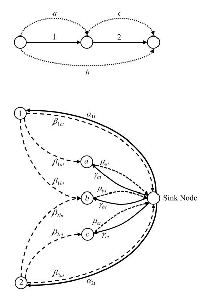
\includegraphics[width=3in]{chap1/figures/mincost.pdf}
\caption{Minimum-cost network flow problem corresponding to problem (\ref{eqn:cond}).}
\end{center}
\end{figure}


\begin{figure}
\begin{center}
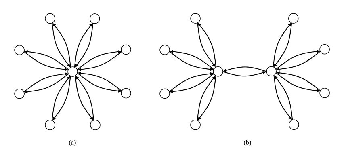
\includegraphics[width=6in]{chap1/figures/network.pdf}
\caption{Structure of the airline network with one and two hubs for the case with $N=8$.}
\label{fig:network}

\end{center}
\end{figure}

\begin{table}
\begin{center}
\footnotesize
\begin{tabular}{|rcc|rrrr|rrrr|rr|}
\hline
\multicolumn{3}{|c|}{} & \multicolumn{4}{c|}{Cons. gen. for prob. (\ref{eqn:alp})} & \multicolumn{4}{c|}{Cons. gen. for prob. (\ref{eqn:cont})} & \multicolumn{2}{c|}{Ratio of secs.} \\
 \multicolumn{3}{|c|}{Test problem} & \multicolumn{1}{|c}{Total} & \multicolumn{1}{c}{1\%} & \multicolumn{1}{c}{\!\!\!\!\% cons.\!\!\!\!} & \multicolumn{1}{c|}{\#} & \multicolumn{1}{|c}{Total} & \multicolumn{1}{c}{1\%} & \multicolumn{1}{c}{\!\!\!\!\% cons.\!\!\!\!} & \multicolumn{1}{c|}{\#} & \multicolumn{1}{c}{Total} & \multicolumn{1}{c|}{1\%}\\
$(\tau,$\!\!&\!\! $N,$ \!\!\!&\!\!\! $\alpha)$ & \multicolumn{1}{c}{secs.} & \multicolumn{1}{c}{secs.} & \multicolumn{1}{c}{gen.} & \multicolumn{1}{c|}{cons.} & \multicolumn{1}{c}{secs.} & \multicolumn{1}{c}{secs.} & \multicolumn{1}{c}{gen.} & \multicolumn{1}{c|}{cons.} & \multicolumn{1}{c}{secs.} & \multicolumn{1}{c|}{secs.} \\
\hline
\hline
(600,\!\!\!\!\!\!&\!\!\!\!\!\!8,\!\!\!\!\!\!&\!\!\!\!\!\!1.0)	&	27.95	&	12.70	&	14.45	&	1,587	&	1.96	&	0.48	&	16.84	&	2,181	&	14.26	&	26.46	\\
(600,\!\!\!\!\!\!&\!\!\!\!\!\!8,\!\!\!\!\!\!&\!\!\!\!\!\!1.3)	&	134.61	&	37.84	&	8.86	&	3,754	&	3.09	&	0.53	&	11.33	&	2,190	&	43.56	&	71.40	\\
(600,\!\!\!\!\!\!&\!\!\!\!\!\!8,\!\!\!\!\!\!&\!\!\!\!\!\!1.6)	&	163.79	&	61.85	&	7.68	&	4,640	&	2.48	&	2.11	&	12.90	&	2,241	&	66.04	&	29.31	\\
\hline
(600,\!\!\!\!\!\!&\!\!\!\!\!\!12,\!\!\!\!\!\!&\!\!\!\!\!\!1.0)	&	181.00	&	23.34	&	14.41	&	3,616	&	9.09	&	1.22	&	8.03	&	6,978	&	19.91	&	19.13	\\
(600,\!\!\!\!\!\!&\!\!\!\!\!\!12,\!\!\!\!\!\!&\!\!\!\!\!\!1.3)	&	476.16	&	114.73	&	11.51	&	7,007	&	14.83	&	13.06	&	5.12	&	8,107	&	32.11	&	8.78	\\
(600,\!\!\!\!\!\!&\!\!\!\!\!\!12,\!\!\!\!\!\!&\!\!\!\!\!\!1.6)	&	582.61	&	159.20	&	11.37	&	7,894	&	15.64	&	14.02	&	4.86	&	7,480	&	37.25	&	11.36	\\
\hline
(800,\!\!\!\!\!\!&\!\!\!\!\!\!8,\!\!\!\!\!\!&\!\!\!\!\!\!1.0)	&	33.06	&	22.83	&	10.74	&	1,793	&	2.49	&	0.75	&	17.27	&	2,066	&	13.28	&	30.44	\\
(800,\!\!\!\!\!\!&\!\!\!\!\!\!8,\!\!\!\!\!\!&\!\!\!\!\!\!1.3)	&	232.19	&	72.45	&	6.88	&	4,719	&	2.96	&	0.83	&	15.88	&	2,176	&	78.44	&	87.29	\\
(800,\!\!\!\!\!\!&\!\!\!\!\!\!8,\!\!\!\!\!\!&\!\!\!\!\!\!1.6)	&	298.00	&	117.37	&	5.47	&	6,137	&	3.21	&	0.81	&	13.40	&	2,241	&	92.83	&	144.90	\\
\hline
(800,\!\!\!\!\!\!&\!\!\!\!\!\!12,\!\!\!\!\!\!&\!\!\!\!\!\!1.0)	&	266.51	&	42.30	&	12.28	&	4,315	&	9.47	&	1.81	&	10.56	&	7,546	&	28.14	&	23.37	\\
(800,\!\!\!\!\!\!&\!\!\!\!\!\!12,\!\!\!\!\!\!&\!\!\!\!\!\!1.3)	&	773.73	&	238.70	&	8.96	&	7,403	&	12.69	&	1.97	&	7.96	&	7,309	&	60.97	&	121.17	\\
(800,\!\!\!\!\!\!&\!\!\!\!\!\!12,\!\!\!\!\!\!&\!\!\!\!\!\!1.6)	&	975.30	&	306.42	&	8.89	&	9,267	&	22.15	&	20.74	&	4.61	&	7,471	&	44.03	&	14.77	\\
\hline
(1000,\!\!\!\!\!\!&\!\!\!\!\!\!8,\!\!\!\!\!\!&\!\!\!\!\!\!1.0)	&	58.15	&	38.53	&	9.36	&	2,231	&	2.72	&	1.00	&	20.59	&	2,336	&	21.38	&	38.53	\\
(1000,\!\!\!\!\!\!&\!\!\!\!\!\!8,\!\!\!\!\!\!&\!\!\!\!\!\!1.3)	&	376.62	&	118.89	&	4.54	&	5,593	&	3.79	&	1.02	&	14.78	&	2,173	&	99.37	&	116.56	\\
(1000,\!\!\!\!\!\!&\!\!\!\!\!\!8,\!\!\!\!\!\!&\!\!\!\!\!\!1.6)	&	451.43	&	201.08	&	4.39	&	7,166	&	3.34	&	1.01	&	16.47	&	2,268	&	135.16	&	199.09	\\
\hline
(1000,\!\!\!\!\!\!&\!\!\!\!\!\!12,\!\!\!\!\!\!&\!\!\!\!\!\!1.0)	&	378.42	&	63.48	&	9.46	&	4,459	&	11.39	&	2.39	&	10.80	&	7,750	&	33.22	&	26.56	\\
(1000,\!\!\!\!\!\!&\!\!\!\!\!\!12,\!\!\!\!\!\!&\!\!\!\!\!\!1.3)	&	1243.83	&	414.68	&	6.35	&	9,356	&	22.09	&	3.21	&	5.57	&	7,779	&	56.31	&	129.18	\\
(1000,\!\!\!\!\!\!&\!\!\!\!\!\!12,\!\!\!\!\!\!&\!\!\!\!\!\!1.6)	&	1556.90	&	408.71	&	6.23	&	11,265	&	20.84	&	2.60	&	5.95	&	7,476	&	74.71	&	157.20	\\
\hline
\multicolumn{11}{|l|}{Average} & 52.83 & 69.75\\
\hline
\end{tabular}
\caption{Computational results for the test problems with one hub.}
\label{tab:one_hub}
\end{center}
\end{table}


\begin{table}
\begin{center}
\footnotesize
\begin{tabular}{|rcc|rrrr|rrrr|rr|}
\hline
\multicolumn{3}{|c|}{} & \multicolumn{4}{c|}{Cons. gen. for prob. (\ref{eqn:alp})} & \multicolumn{4}{c|}{Cons. gen. for prob. (\ref{eqn:cont})} & \multicolumn{2}{c|}{Ratio of secs.} \\
 \multicolumn{3}{|c|}{Test problem} & \multicolumn{1}{|c}{Total} & \multicolumn{1}{c}{1\%} & \multicolumn{1}{c}{\!\!\!\!\% cons.\!\!\!\!} & \multicolumn{1}{c|}{\#} & \multicolumn{1}{|c}{Total} & \multicolumn{1}{c}{1\%} & \multicolumn{1}{c}{\!\!\!\!\% cons.\!\!\!\!} & \multicolumn{1}{c|}{\#} & \multicolumn{1}{c}{Total} & \multicolumn{1}{c|}{1\%}\\
$(\tau,$\!\!&\!\! $N,$ \!\!\!&\!\!\! $\alpha)$ & \multicolumn{1}{c}{secs.} & \multicolumn{1}{c}{secs.} & \multicolumn{1}{c}{gen.} & \multicolumn{1}{c|}{cons.} & \multicolumn{1}{c}{secs.} & \multicolumn{1}{c}{secs.} & \multicolumn{1}{c}{gen.} & \multicolumn{1}{c|}{cons.} & \multicolumn{1}{c}{secs.} & \multicolumn{1}{c|}{secs.} \\
\hline
\hline
(600,\!\!\!\!\!\!&\!\!\!\!\!\!8,\!\!\!\!\!\!&\!\!\!\!\!\!1.0)	&	71.60	&	14.50	&	13.63	&	2,530	&	3.43	&	0.71	&	11.95	&	3,963	&	20.87	&	20.42		\\
(600,\!\!\!\!\!\!&\!\!\!\!\!\!8,\!\!\!\!\!\!&\!\!\!\!\!\!1.3)	&	188.40	&	46.57	&	7.99	&	5,162	&	3.49	&	0.69	&	12.03	&	3,253	&	53.98	&	67.49		\\
(600,\!\!\!\!\!\!&\!\!\!\!\!\!8,\!\!\!\!\!\!&\!\!\!\!\!\!1.6)	&	249.05	&	64.55	&	7.69	&	6,447	&	5.45	&	0.70	&	7.71	&	3,212	&	45.70	&	92.21		\\
\hline
(600,\!\!\!\!\!\!&\!\!\!\!\!\!12,\!\!\!\!\!\!&\!\!\!\!\!\!1.0)	&	205.05	&	27.80	&	13.76	&	3,820	&	5.57	&	1.56	&	14.90	&	10,794	&	36.81	&	17.82		\\
(600,\!\!\!\!\!\!&\!\!\!\!\!\!12,\!\!\!\!\!\!&\!\!\!\!\!\!1.3)	&	645.48	&	184.92	&	10.31	&	7,636	&	16.54	&	1.56	&	5.02	&	10,108	&	39.03	&	118.54		\\
(600,\!\!\!\!\!\!&\!\!\!\!\!\!12,\!\!\!\!\!\!&\!\!\!\!\!\!1.6)	&	893.31	&	208.37	&	13.87	&	9,747	&	30.57	&	21.17	&	2.72	&	9,654	&	29.22	&	9.84		\\
\hline
(800,\!\!\!\!\!\!&\!\!\!\!\!\!8,\!\!\!\!\!\!&\!\!\!\!\!\!1.0)	&	115.27	&	25.83	&	12.01	&	3,049	&	3.89	&	1.03	&	13.88	&	3,905	&	29.63	&	25.08		\\
(800,\!\!\!\!\!\!&\!\!\!\!\!\!8,\!\!\!\!\!\!&\!\!\!\!\!\!1.3)	&	280.69	&	81.41	&	6.91	&	5,420	&	5.37	&	0.98	&	10.06	&	3,234	&	52.27	&	83.07		\\
(800,\!\!\!\!\!\!&\!\!\!\!\!\!8,\!\!\!\!\!\!&\!\!\!\!\!\!1.6)	&	470.34	&	121.14	&	5.19	&	8,502	&	5.32	&	1.00	&	10.34	&	3,234	&	88.41	&	121.14		\\
\hline
(800,\!\!\!\!\!\!&\!\!\!\!\!\!12,\!\!\!\!\!\!&\!\!\!\!\!\!1.0)	&	269.02	&	49.32	&	9.07	&	3,464	&	8.41	&	2.16	&	13.08	&	10,896	&	31.99	&	22.83		\\
(800,\!\!\!\!\!\!&\!\!\!\!\!\!12,\!\!\!\!\!\!&\!\!\!\!\!\!1.3)	&	1108.39	&	239.38	&	8.43	&	9,322	&	29.66	&	2.18	&	3.71	&	9,961	&	37.37	&	109.81		\\
(800,\!\!\!\!\!\!&\!\!\!\!\!\!12,\!\!\!\!\!\!&\!\!\!\!\!\!1.6)	&	1587.84	&	396.69	&	9.89	&	11,686	&	33.38	&	30.93	&	4.37	&	9,639	&	47.57	&	12.83		\\
\hline
(1000,\!\!\!\!\!\!&\!\!\!\!\!\!8,\!\!\!\!\!\!&\!\!\!\!\!\!1.0)	&	119.30	&	43.80	&	14.74	&	2,583	&	3.55	&	1.32	&	19.44	&	3,811	&	33.61	&	33.18		\\
(1000,\!\!\!\!\!\!&\!\!\!\!\!\!8,\!\!\!\!\!\!&\!\!\!\!\!\!1.3)	&	422.91	&	130.35	&	5.51	&	6,146	&	5.79	&	1.30	&	12.61	&	3,183	&	73.04	&	100.27		\\
(1000,\!\!\!\!\!\!&\!\!\!\!\!\!8,\!\!\!\!\!\!&\!\!\!\!\!\!1.6)	&	758.49	&	196.56	&	3.92	&	10,524	&	7.58	&	1.29	&	8.84	&	3,233	&	100.06	&	152.37		\\
\hline
(1000,\!\!\!\!\!\!&\!\!\!\!\!\!12,\!\!\!\!\!\!&\!\!\!\!\!\!1.0)	&	405.09	&	76.06	&	6.81	&	4,148	&	7.80	&	2.82	&	17.82	&	10,946	&	51.93	&	26.97		\\
(1000,\!\!\!\!\!\!&\!\!\!\!\!\!12,\!\!\!\!\!\!&\!\!\!\!\!\!1.3)	&	1909.78	&	411.63	&	5.73	&	12,112	&	22.58	&	2.83	&	6.16	&	9,235	&	84.58	&	145.45		\\
(1000,\!\!\!\!\!\!&\!\!\!\!\!\!12,\!\!\!\!\!\!&\!\!\!\!\!\!1.6)	&	1931.23	&	449.95	&	9.80	&	15,925	&	30.44	&	2.87	&	4.53	&	9,697	&	63.44	&	156.78		\\
\hline
\multicolumn{11}{|l|}{Average} & 51.08 & 73.12\\
\hline
\end{tabular}

\caption{Computational results for the test problems with two hubs.}
\label{tab:two_hubs}

\end{center}
\end{table}


\begin{table}
\begin{center}
\footnotesize
\begin{tabular}{|rcc|rr|rr|}
\hline
\multicolumn{3}{|c|}{} & \multicolumn{2}{c|}{Cons. gen.} & \multicolumn{2}{c|}{Dir. solut.}\\
\multicolumn{3}{|c|}{} & \multicolumn{2}{c|}{for prob. (\ref{eqn:cont})} & \multicolumn{2}{c|}{for prob. (\ref{eqn:cont})} \\
 \multicolumn{3}{|c|}{Test problem} & \multicolumn{1}{|c}{Total} & \multicolumn{1}{c|}{1\%} & \multicolumn{1}{|c}{Total} & \multicolumn{1}{c|}{1\%} \\
$(\tau,$\!\!&\!\! $N,$ \!\!\!&\!\!\! $\alpha)$ & \multicolumn{1}{c}{secs.} & \multicolumn{1}{c|}{secs.} & \multicolumn{1}{c}{secs.} & \multicolumn{1}{c|}{secs.}  \\
\hline
\hline
(600,\!\!\!\!\!\!&\!\!\!\!\!\!8,\!\!\!\!\!\!&\!\!\!\!\!\!1.0)	&	1.96	&	0.48	&	1.01	&	0.81	\\
(600,\!\!\!\!\!\!&\!\!\!\!\!\!8,\!\!\!\!\!\!&\!\!\!\!\!\!1.3)	&	3.09	&	0.53	&	2.94	&	1.82	\\
(600,\!\!\!\!\!\!&\!\!\!\!\!\!8,\!\!\!\!\!\!&\!\!\!\!\!\!1.6)	&	2.48	&	2.11	&	3.56	&	2.09	\\
\hline
(600,\!\!\!\!\!\!&\!\!\!\!\!\!12,\!\!\!\!\!\!&\!\!\!\!\!\!1.0)	&	9.09	&	1.22	&	8.52	&	3.00	\\
(600,\!\!\!\!\!\!&\!\!\!\!\!\!12,\!\!\!\!\!\!&\!\!\!\!\!\!1.3)	&	14.83	&	13.06	&	22.39	&	7.62	\\
(600,\!\!\!\!\!\!&\!\!\!\!\!\!12,\!\!\!\!\!\!&\!\!\!\!\!\!1.6)	&	15.64	&	14.02	&	36.01	&	9.18	\\
\hline
(800,\!\!\!\!\!\!&\!\!\!\!\!\!8,\!\!\!\!\!\!&\!\!\!\!\!\!1.0)	&	2.49	&	0.75	&	1.79	&	1.46	\\
(800,\!\!\!\!\!\!&\!\!\!\!\!\!8,\!\!\!\!\!\!&\!\!\!\!\!\!1.3)	&	2.96	&	0.83	&	2.82	&	1.95	\\
(800,\!\!\!\!\!\!&\!\!\!\!\!\!8,\!\!\!\!\!\!&\!\!\!\!\!\!1.6)	&	3.21	&	0.81	&	5.99	&	3.61	\\
\hline
(800,\!\!\!\!\!\!&\!\!\!\!\!\!12,\!\!\!\!\!\!&\!\!\!\!\!\!1.0)	&	9.47	&	1.81	&	8.67	&	3.33	\\
(800,\!\!\!\!\!\!&\!\!\!\!\!\!12,\!\!\!\!\!\!&\!\!\!\!\!\!1.3)	&	12.69	&	1.97	&	18.21	&	5.72	\\
(800,\!\!\!\!\!\!&\!\!\!\!\!\!12,\!\!\!\!\!\!&\!\!\!\!\!\!1.6)	&	22.15	&	20.74	&	58.15	&	15.43	\\
\hline
(1000,\!\!\!\!\!\!&\!\!\!\!\!\!8,\!\!\!\!\!\!&\!\!\!\!\!\!1.0)	&	2.72	&	1.00	&	4.35	&	3.55	\\
(1000,\!\!\!\!\!\!&\!\!\!\!\!\!8,\!\!\!\!\!\!&\!\!\!\!\!\!1.3)	&	3.79	&	1.02	&	5.32	&	3.21	\\
(1000,\!\!\!\!\!\!&\!\!\!\!\!\!8,\!\!\!\!\!\!&\!\!\!\!\!\!1.6)	&	3.34	&	1.01	&	8.20	&	3.87	\\
\hline
(1000,\!\!\!\!\!\!&\!\!\!\!\!\!12,\!\!\!\!\!\!&\!\!\!\!\!\!1.0)	&	11.39	&	2.39	&	9.17	&	4.82	\\
(1000,\!\!\!\!\!\!&\!\!\!\!\!\!12,\!\!\!\!\!\!&\!\!\!\!\!\!1.3)	&	22.09	&	3.21	&	45.38	&	10.62	\\
(1000,\!\!\!\!\!\!&\!\!\!\!\!\!12,\!\!\!\!\!\!&\!\!\!\!\!\!1.6)	&	20.84	&	2.60	&	82.29	&	11.27	\\
\hline
\end{tabular}
~~~~~~
\begin{tabular}{|rcc|rr|rr|}
\hline
\multicolumn{3}{|c|}{} & \multicolumn{2}{c|}{Cons. gen.} & \multicolumn{2}{c|}{Dir. solut.}\\
\multicolumn{3}{|c|}{} & \multicolumn{2}{c|}{for prob. (\ref{eqn:cont})} & \multicolumn{2}{c|}{for prob. (\ref{eqn:cont})} \\
 \multicolumn{3}{|c|}{Test problem} & \multicolumn{1}{|c}{Total} & \multicolumn{1}{c|}{1\%} & \multicolumn{1}{|c}{Total} & \multicolumn{1}{c|}{1\%} \\
$(\tau,$\!\!&\!\! $N,$ \!\!\!&\!\!\! $\alpha)$ & \multicolumn{1}{c}{secs.} & \multicolumn{1}{c|}{secs.} & \multicolumn{1}{c}{secs.} & \multicolumn{1}{c|}{secs.}  \\
\hline
\hline
(600,\!\!\!\!\!\!&\!\!\!\!\!\!8,\!\!\!\!\!\!&\!\!\!\!\!\!1.0)	&	3.43	&	0.71	&	1.79	&	0.78	\\
(600,\!\!\!\!\!\!&\!\!\!\!\!\!8,\!\!\!\!\!\!&\!\!\!\!\!\!1.3)	&	3.49	&	0.69	&	3.48	&	1.62	\\
(600,\!\!\!\!\!\!&\!\!\!\!\!\!8,\!\!\!\!\!\!&\!\!\!\!\!\!1.6)	&	5.45	&	0.70	&	6.06	&	2.42	\\
\hline
(600,\!\!\!\!\!\!&\!\!\!\!\!\!12,\!\!\!\!\!\!&\!\!\!\!\!\!1.0)	&	5.57	&	1.56	&	5.51	&	1.90	\\
(600,\!\!\!\!\!\!&\!\!\!\!\!\!12,\!\!\!\!\!\!&\!\!\!\!\!\!1.3)	&	16.54	&	1.56	&	27.16	&	9.43	\\
(600,\!\!\!\!\!\!&\!\!\!\!\!\!12,\!\!\!\!\!\!&\!\!\!\!\!\!1.6)	&	30.57	&	21.17	&	47.57	&	12.61	\\
\hline
(800,\!\!\!\!\!\!&\!\!\!\!\!\!8,\!\!\!\!\!\!&\!\!\!\!\!\!1.0)	&	3.89	&	1.03	&	2.16	&	1.87	\\
(800,\!\!\!\!\!\!&\!\!\!\!\!\!8,\!\!\!\!\!\!&\!\!\!\!\!\!1.3)	&	5.37	&	0.98	&	5.71	&	1.81	\\
(800,\!\!\!\!\!\!&\!\!\!\!\!\!8,\!\!\!\!\!\!&\!\!\!\!\!\!1.6)	&	5.32	&	1.00	&	8.11	&	4.17	\\
\hline
(800,\!\!\!\!\!\!&\!\!\!\!\!\!12,\!\!\!\!\!\!&\!\!\!\!\!\!1.0)	&	8.41	&	2.16	&	6.18	&	3.42	\\
(800,\!\!\!\!\!\!&\!\!\!\!\!\!12,\!\!\!\!\!\!&\!\!\!\!\!\!1.3)	&	29.66	&	2.18	&	56.74	&	6.60	\\
(800,\!\!\!\!\!\!&\!\!\!\!\!\!12,\!\!\!\!\!\!&\!\!\!\!\!\!1.6)	&	33.38	&	30.93	&	83.88	&	17.36	\\
\hline
(1000,\!\!\!\!\!\!&\!\!\!\!\!\!8,\!\!\!\!\!\!&\!\!\!\!\!\!1.0)	&	3.55	&	1.32	&	4.96	&	1.47	\\
(1000,\!\!\!\!\!\!&\!\!\!\!\!\!8,\!\!\!\!\!\!&\!\!\!\!\!\!1.3)	&	5.79	&	1.30	&	4.51	&	2.35	\\
(1000,\!\!\!\!\!\!&\!\!\!\!\!\!8,\!\!\!\!\!\!&\!\!\!\!\!\!1.6)	&	7.58	&	1.29	&	10.52	&	4.36	\\
\hline
(1000,\!\!\!\!\!\!&\!\!\!\!\!\!12,\!\!\!\!\!\!&\!\!\!\!\!\!1.0)	&	7.8	&	2.82	&	8.71	&	3.43	\\
(1000,\!\!\!\!\!\!&\!\!\!\!\!\!12,\!\!\!\!\!\!&\!\!\!\!\!\!1.3)	&	22.58	&	2.83	&	53.38	&	7.34	\\
(1000,\!\!\!\!\!\!&\!\!\!\!\!\!12,\!\!\!\!\!\!&\!\!\!\!\!\!1.6)	&	30.44	&	2.87	&	110.58	&	14.19	\\
\hline
\end{tabular}

\caption{CPU seconds for problem (\ref{eqn:cont}) when we solve this problem by using constraint generation and when we solve this problem directly by using a linear programming solver.}
\label{tab:direct}
\end{center}
\end{table}




\begin{table}
\begin{center}
\footnotesize
\begin{tabular}{|rcc|rr|}
\hline
\multicolumn{3}{|c|}{} & \multicolumn{2}{c|}{Cons. gen.} \\
\multicolumn{3}{|c|}{} & \multicolumn{2}{c|}{for prob. (\ref{eqn:cont})} \\
 \multicolumn{3}{|c|}{Test problem} & \multicolumn{1}{|c}{Total} & \multicolumn{1}{c|}{1\%} \\
$(\tau,$\!\!&\!\! $N,$ \!\!\!&\!\!\! $\alpha)$ & \multicolumn{1}{c}{secs.} & \multicolumn{1}{c|}{secs.}  \\
\hline
\hline
(600,\!\!\!\!\!\!&\!\!\!\!\!\!20,\!\!\!\!\!\!&\!\!\!\!\!\!1.0)	&	34.77	&	3.69	\\
(600,\!\!\!\!\!\!&\!\!\!\!\!\!20,\!\!\!\!\!\!&\!\!\!\!\!\!1.3)	&	42.07	&	9.19	\\
(600,\!\!\!\!\!\!&\!\!\!\!\!\!20,\!\!\!\!\!\!&\!\!\!\!\!\!1.6)	&	54.17	&	12.93	\\
\hline
(600,\!\!\!\!\!\!&\!\!\!\!\!\!24,\!\!\!\!\!\!&\!\!\!\!\!\!1.0)	&	151.56	&	5.02	\\
(600,\!\!\!\!\!\!&\!\!\!\!\!\!24,\!\!\!\!\!\!&\!\!\!\!\!\!1.3)	&	124.70	&	20.69	\\
(600,\!\!\!\!\!\!&\!\!\!\!\!\!24,\!\!\!\!\!\!&\!\!\!\!\!\!1.6)	&	120.11	&	50.57	\\
\hline
\end{tabular}
~~~~
\begin{tabular}{|rcc|rr|}
\hline
\multicolumn{3}{|c|}{} & \multicolumn{2}{c|}{Cons. gen.} \\
\multicolumn{3}{|c|}{} & \multicolumn{2}{c|}{for prob. (\ref{eqn:cont})} \\
 \multicolumn{3}{|c|}{Test problem} & \multicolumn{1}{|c}{Total} & \multicolumn{1}{c|}{1\%} \\
$(\tau,$\!\!&\!\! $N,$ \!\!\!&\!\!\! $\alpha)$ & \multicolumn{1}{c}{secs.} & \multicolumn{1}{c|}{secs.}  \\
\hline
\hline
(800,\!\!\!\!\!\!&\!\!\!\!\!\!20,\!\!\!\!\!\!&\!\!\!\!\!\!1.0)	&	37.69	&	4.71	\\
(800,\!\!\!\!\!\!&\!\!\!\!\!\!20,\!\!\!\!\!\!&\!\!\!\!\!\!1.3)	&	62.11	&	5.06	\\
(800,\!\!\!\!\!\!&\!\!\!\!\!\!20,\!\!\!\!\!\!&\!\!\!\!\!\!1.6)	&	74.30	&	11.21	\\
\hline
(800,\!\!\!\!\!\!&\!\!\!\!\!\!24,\!\!\!\!\!\!&\!\!\!\!\!\!1.0)	&	80.79	&	6.84	\\
(800,\!\!\!\!\!\!&\!\!\!\!\!\!24,\!\!\!\!\!\!&\!\!\!\!\!\!1.3)	&	96.69	&	18.66	\\
(800,\!\!\!\!\!\!&\!\!\!\!\!\!24,\!\!\!\!\!\!&\!\!\!\!\!\!1.6)	&	454.20	&	26.17	\\
\hline
\end{tabular}
~~~~
\begin{tabular}{|rcc|rr|}
\hline
\multicolumn{3}{|c|}{} & \multicolumn{2}{c|}{Cons. gen.} \\
\multicolumn{3}{|c|}{} & \multicolumn{2}{c|}{for prob. (\ref{eqn:cont})} \\
 \multicolumn{3}{|c|}{Test problem} & \multicolumn{1}{|c}{Total} & \multicolumn{1}{c|}{1\%} \\
$(\tau,$\!\!&\!\! $N,$ \!\!\!&\!\!\! $\alpha)$ & \multicolumn{1}{c}{secs.} & \multicolumn{1}{c|}{secs.}  \\
\hline
\hline
(1000,\!\!\!\!\!\!&\!\!\!\!\!\!20,\!\!\!\!\!\!&\!\!\!\!\!\!1.0)	&	46.67	&	5.96	\\
(1000,\!\!\!\!\!\!&\!\!\!\!\!\!20,\!\!\!\!\!\!&\!\!\!\!\!\!1.3)	&	78.63	&	6.00	\\
(1000,\!\!\!\!\!\!&\!\!\!\!\!\!20,\!\!\!\!\!\!&\!\!\!\!\!\!1.6)	&	66.77	&	12.13	\\
\hline
(1000,\!\!\!\!\!\!&\!\!\!\!\!\!24,\!\!\!\!\!\!&\!\!\!\!\!\!1.0)	&	85.91	&	8.69	\\
(1000,\!\!\!\!\!\!&\!\!\!\!\!\!24,\!\!\!\!\!\!&\!\!\!\!\!\!1.3)	&	164.79	&	8.93	\\
(1000,\!\!\!\!\!\!&\!\!\!\!\!\!24,\!\!\!\!\!\!&\!\!\!\!\!\!1.6)	&	143.18	&	26.87	\\
\hline
\end{tabular}

\caption{CPU seconds for problem (\ref{eqn:cont}) for large test problems.}
\label{tab:large}
\end{center}
\end{table}


\chapter{Facility Location with Types}

\section{Introduction}

Although algorithm design for the {\it facility location problem} and its many variants has been the focus of a significant body of research, there is an important class of generalizations that has received much attention, but only with more limited success. In the facility location problem, one has a set of demand points and a set of potential facility locations, with specified costs for opening, and the aim is to optimize the choice of open facilities so as to minimize the sum of opening costs and the cost of assigning each demand point to an open facility, where the assignment costs derive from an underlying metric space containing all of the locations. This model places no restrictions on the clients served by each facility, which is typically an unreasonable assumption, and so a great deal of work has been done to address further constrained models. The simplest extension is to impose a capacity constraint, but for a wide range of applications, it is more appropriate to distinguish types of service provided and required, and it is on this class of problems that we shall focus. Facility location models are closely linked to a number of inventory models, since one can view a facility as a point in time at which an order is placed, and the assignment cost then corresponds to the cost of filling a particular demand from that order, where one can have fixed ordering costs, unit ordering costs, and inventory holding costs easily incorporated into this setting. In this chapter, we shall consider both facility location and inventory management problems that arise in the setting with type constraints. 

Since the facility location problem is NP-hard, much of the algorithmic work in this domain has focused on the design of approximation algorithms, and it has proved to be a fertile ground for the development of many of the now-standard techniques in algorithm design:
researchers have applied deterministic and randomized rounding \cite{shmoys1997approximation,li20131,chudak2003improved}, primal-dual methods \cite{jain2001approximation}, local search\cite{korupolu2000analysis}, and even greedy-type algorithms \cite{jain2003greedy} to this problem. For the classical facility location problem, the best approximation guarantee currently known is a 1.488-approximation algorithm (where a {\it $\rho$-approximation algorithm} is a polynomial-time algorithm that is guaranteed to find a feasible solution of objective function value within a factor of $\rho$ of the optimum), which was obtained by randomized rounding \cite{li20131}.
For the {\it $k$-median problem}, in which there are no facility costs but one is limited to opening only $k$ facilities, strong results are known via a range of techniques as well \cite{li2013approximating,jain2001approximation,arya2004local}, and analogous results (though more limited) are known for the capacitated version of the facility location problem \cite{chudak2005improved,an2014lp,pal2001facility,bansal20125}. One particularly notable open problem is to derive good algorithms for the setting in which the opening/ordering costs are submodular set functions of the set of demand points assigned (or for suitably general special cases).

The research presented here aims to derive results in which each facility may have a
different serving capability. In the most general case along these lines, for each client,
we can specify the set of facilities that can serve it. However, it is easy to reduce the
set cover problem to it in an approximation-preserving manner (see appendix); thus, approximation
hardness results known for the set cover problem would apply (and hence no sub-logarithmic
guarantee is possible unless P=NP). Hence, the issue is to model sufficiently robust
classes of problems that capture interesting application settings, and yet by-pass this
hardness result.  We consider the following classes of problems, in which  each facility
and client is assigned a type, and there is a specified partial ordering among types so
that a client must be served by any open facility of equal or higher type.  
The structure of the partial ordering will determine the nature of our problems. 
With a general partial order, one can again reduce set cover to the problem; we consider
two structured variants to bypass this. 

\begin{itemize}
\item \textbf{Facility Location with Hierarchical Types.} In this problem, the types form a rooted tree in which a facility of a given type can serve any client that has a type that is a descendant of the facility type in the tree (where a node is trivially a descendant of itself).

\item \textbf{Pepsi-Coke Facility Location.} In this problem, there are only two types of facilities: Pepsi facilities and Coke facilities. There are three types of clients: Pepsi clients, Coke clients and Anything-will-do clients. As the names suggest, Anything-will-do clients can be served by any facility, but the other clients can only be served by facilities of the same type. The partial ordering here is a ``V-shape,'' where there are no facilities of the bottom type.

\end{itemize}

A model somewhat weaker than the former setting was considered by Barman and
Chawla~\cite{DBLP:journals/corr/abs-1110-4150}, who introduced a problem called the {\it
  redundancy-aware facility location problem}, where each client needs a set of services
and all of these services need to be installed at the same facility location in order to
serve that client; they gave an LP rounding algorithm with approximation guarantee of 27
for the case that all clients' demanded service sets are laminar. The facility location
problem with hierarchical types is the generalization of their problem if we group
services belong to the same service set to a single facility. We include more details on the relationship in appendix. In contrast, the first main
result of this chapter is a simple primal-dual 3-approximation algorithm for the facility
location problem with hierarchical types. We show how to add a simple prioritization rule
to the pruning phase of the algorithm of Jain and Vazirani \cite{jain2001approximation}
leads to this result. Furthermore, the analysis gives a stronger result; we show that it
is a Lagrangian-multiplier-preserving algorithm, in that not only is the sum of the
assignment and facility costs at most three times the optimum, but the sum of the
assignment and 3 times the facility cost is at most 3 times the optimal cost. We are
unable to convert this to an analogous $k$-median result, but we can augment this analysis with a rescaling technique \mbox{to obtain a 1.85-approximation algorithm.}

For the Pepsi-Coke facility location problem, we add a new dimension to the by-now standard LP rounding-by-clustering techniques that arises due to the fact that when choosing a cluster for one of the Anything-will-do clients $j$, a facility used by the LP solution for that client, cannot necessarily serve all of the clients served by any facility fractionally serving $j$. We overcome this difficulty by separately performing two clustering constructions,  but then couple the outcomes by relying on an auxiliary matroid intersection computation, where a feasible fractional solution to the matroid intersection instance is derived from the original fractional solution (in a manner similar to a technique used by Swamy \cite{swamy2013improved}). Consequently, we obtain a 3-approximation algorithm for the Pepsi-Coke facility location problem.

Analogous to the development of approximation algorithms for facility location problems,
there has been a corresponding thread of research investigating results of a variety of
inventory management problems, primarily the {\it lot-sizing} and the {\it joint
  replenishment
  problem}\cite{levi2008approximation,levi2008constant,levi2006primal,ApproxjrpD:Beinkowski,cheung2014submodular}. In
some elements, these problems are sometimes simpler than their facility location
equivalents, since the assignment costs, in addition to obeying the triangle inequality,
often have an even more refined structure due to the linear nature of ordering/demand time
periods. However, these problems have a harder element, since the metric is definitely not
symmetric - one cannot serve a demand point earlier in time than the ordering
period. Hence, it is natural to ask for the analogs of the two results discussed above. Surprisingly, for the lot-sizing problem with hierarchical types, we show that the problem can be solved dynamic programming in polynomial time, in a manner exactly analogous to a recent result \cite{cheung2014submodular}. However, unlike for the unconstrained lot-sizing problem, for which the natural linear programming relaxation is the basis for a primal-dual polynomial-time algorithm as well \cite{levi2006primal},
we give an example for which there is an integrality gap of 4/3 for the lot-sizing problem with hierarchical types.

\section{Preliminaries}

In this section, we introduce some definitions and notation to be used throughout this paper.

Let $\mathcal{F}$ be the set of potential facilities that we can open; opening facility $i \in \mathcal{F}$ has associated non-negative cost $f_i$.
There is also a set of clients $\mathcal{D}$ requiring services. We need to assign each client $j \in \mathcal{C}$ to an open facility.
The connection cost to serve client $j\in \mathcal{D}$ by facility $i \in \mathcal{F}$ is $c_{ij}$.
We assume $c_{ij}$ forms a metric and thus triangular inequality holds.

In addition, there is set of types $\mathcal{T}$. These types form some partial ordering. Each facility $i$ has a type $t(i)$ indicating its serving capability. Each client also has a type $t(j)$ specifying its require level. It's required in the solution that any client $j$ is served only by facility $i$ of equal or higher type, i.e. $t(j) \le t(i)$. Denote $\mathcal{F}(j)$ be all facilities that can serve client $j$.

Suppose in the solution, we opened the set of facilities $S$ and we assign client $j$ to $\sigma(j)$. Then the total cost of this solution is
\[  \sum_{i \in S} f_i + \sum_{j \in \mathcal{D}} c_{\sigma(j)j}    \]
The first part is total facility opening cost and the second part is total connection cost. The goal is to find a feasible solution with minimum total cost.

Our algorithm and analysis will use linear programming formulations of this problem. We describe them here. The following is the natural linear programming relaxation.

\begin{align}
\min \quad & \sum_{i \in \mathcal{F}} f_i y_i + \sum_{j \in \mathcal{D}} \sum_{i \in \mathcal{F}(j)} c_{ij}x_{ij} \label{LP:main} \\
\text{s.t.} \quad & \sum_{i \in \mathcal{F}(j)} x_{ij} \ge 1 \quad \forall {j \in \mathcal{D}} \label{con:P:demand}\\
& x_{ij} \le y_i    \quad \forall j \in \mathcal{D}, i \in \mathcal{F}(j)   \label{con:P:reliance}\\
& y_i \ge 0 \quad \forall {i \in \mathcal{F}}   \label{con:P:ynonneg}\\
& x_{ij} \ge 0 \quad \forall j \in \mathcal{D}, i \in \mathcal{F}(j) \label{con:P:xnonneg}
\end{align}

Any binary feasible solution would corresponds to a feasible solution. $y_i = 1$ indicates that facility $i$ is open and $x_{ij} = 1$ indicates that client $j$ is served by facility $i$. The set of constraints ensure that we assign the client to a facility which compatible types. Taking the dual, we get the following

\begin{align}
\max \quad & \sum_{j \in \mathcal{D}} v_j \\
\text{s.t.} \quad & v_j \le c_{ij} + w_{ij} \quad \forall j \in \mathcal{D}, i \in \mathcal{F}(j)\\
& \sum_{j: i \in \mathcal{F}(j)} w_{ij} \le f_i \quad \forall i \in \mathcal{F} \\
& w_{ij} \ge 0  \quad \forall j \in \mathcal{D}, i \in \mathcal{F}(j) \label{con:facility} \\
& v_j \ge 0 \quad \forall j \in \mathcal{D}
\end{align}

Here we can intuitively think $v_j$ as budget of client $j$ and $w_{ij}$ as how much client $j$ contributes towards opening facility $i$. The first set of constraints say that the budget can be  to cover both connection cost and contribution toward opening facilities. The second set of constraints say that the total contribution toward one facility cannot exceed its opening cost.
\section{Facility Location of Hierarchical Types}

Remember in this problem, the types form a tree where the root is on top. The partial ordering between types is specified by ancestor relationship in the tree: a type is lower than all of its ancestors. This models a hierarchical structure where facility higher up in the hierarchy can be used to serve all clients of types in the subtree. We will first present a simple 3-approximation algorithm as extension of classical primal dual algorithm. Then we will show how to combine this with randomized rounding and cost scaling to achieve 1.85-approximation algorithm.

\subsection{Simple 3-approximation algorithm}

The algorithm follows standard Jain-Vazirani \cite{jain2001approximation} approach and operates in two phases.

\paragraph{Dual ascent phase}
In this phase, we construct an feasible solution to the dual linear programming and,
at the same time, a tentative (infeasible) solution to the primal problem.
We will construct an feasible primal solution later based on the tentative solution.

Initially we set all dual variables $v_j = 0$ and all clients are active.
We keep increase $v_j$ for all active clients in uniform rate until one of the following events happens

\begin{itemize}
\item \textbf{Event 1} When $v_j = c_{ij}$, for some $i \in \mathcal{F}(j)$ and $i$ is not tentatively open,
we cannot increase $v_j$ any more without increasing $w_{ij}$.
Thus, we start to increase $w_{ij}$ along with $v_j$ at the same rate.

\item \textbf{Event 2} When $\sum_{j: i \in \mathcal{F}(j)} w_{ij} = f_i$, we cannot increase corresponding $v_j$ any more.
So we tentatively open facility $i$ and mark an active client $j$ inactive if $v_j \ge c_{ij}$ and $i \in \mathcal{F}(j)$.
In this way, we stop to increase $v_j$ for these clients so we don't violate constraints (\ref{con:facility}).

\item \textbf{Event 3} When $v_j = c_{ij}$, for some $i \in \mathcal{F}(j)$ and $i$ is tentatively open,
we mark $j$ to be inactive.
\end{itemize}

The process ends when all clients are inactive.

\begin{defn}
We says client $j$ contributes to facility $i$ if $w_{ij} > 0$.
We says client $j$ is frozen by facility $i$ if we mark $j$ inactive during Event 1 or Event 3.
\end{defn}

Note that for any tentatively open facility $i$, if we take all contributing clients,
their budget can cover opening cost $f_i$ plus their connection cost to $i$.
It seems we can open all tentatively open facilities and assign all clients to the facility frozen it.
However, the problem is that each client can contributes to multiple tentatively open facilities,
thus we can use budget of some clients multiple times, which makes it hard to bound the total facility opening cost.
This is the reason why we need the Pruning Phase to select some facilities to open.

\paragraph{Pruning phase}

In this phase, we consider the type tree $\mathcal{T}$ in top-down fashion,
i.e. we process type $t$ before type $s$ if $t > s$ in the type tree $\mathcal{T}$.
Also we will maintain a set $D$ which is the set of clients that we will use their budgets to cover facility opening cost.
When processing type $t \in \mathcal{T}$, we look at each tentatively open facility $i$ of type $t$.
We permanently open facility $i$ and pay its opening cost $f_i$
if all contributing clients $j$ are not marked centers yet ($j \not \in D$).
Then we mark all contributing clients of facility $i$ to be centers, adding them to $D$.
On the other hand, if there is one contributing client $j \in D$, then we don't open facility $i$ and move to the next facility.

In the end, we assign each client to the closest facility $i$ with $i \in \mathcal{F}(j)$.

\subsection{Analysis}

For our solution, let $F$ be the total facility opening cost and let $C$ be the total connection cost.
Let $OPT$ be the optimal solution's cost.
Now we want to prove the primal dual algorithm is Lagrange Multiplier Preserving 3-approximation, which means
\[  3F + C \le 3 OPT    \]

To demonstrate this, we show a particular way of assigning clients to open facilities will have small cost.
Thus, assigning clients to closest facility which can serve it will result in no more cost.

Remember $D$ is the set of clients marked centers during Pruning Phase.
Let $S$ be the set of facilities that we permanently open in the end.
For each permanently open facility $i \in S$, let $Pay_i$ be the set of its contributing clients.
We know $D = \cup_{i \in S} Pay_i$.
Because of the way we open facilities during Pruning Phase

\begin{fact}
For two permanently open facilities $i, l$, we know $Pay_i, Pay_l$ are disjoint.
\end{fact}

Thus, for any $i \in S$, we can assign $Pay_i$ to $i$.
Note for any $j \in Pay_i$, we know $w_{ij} > 0$ and this implies $i \in \mathcal{F}(j)$ so $i$ is capable of serving $j$.
we can pay for the total cost with the budgets of $Pay_i$ because

\[  f_i = \sum_{j \in Pay_i} w_{ij} = \sum_{j \in Pay_i} (v_j - c_{ij}) \]

Rearranging terms, we get

\[ f_i + \sum_{j \in Pay_i} c_{ij} = \sum_{j \in Pay_i} v_j \]

Since $Pay_i, Pay_l$ are disjoint for different facilities $i, l \in S$, we know we never spend any client twice.

We still need to bound the connection cost of remaining clients $\bar D = \mathcal{D} \backslash D$.

\begin{lem}
For any client $j \in \bar D$, there is a open facility $i \in \mathcal{F}(j)$ and $c_{ij} \le 3v_j$.
\end{lem}

\begin{proof}
Consider the facility $i$ which frozen client $j$. If $i \in S$, then we can just assign $j$ to $i$ and $c_{ij} \le v_j$ and we are done.

If $i$ is not opened, that means there is a client $k$ contributing to both $i$ and some open facility $l$. Since $k$ contributes to $i$, we know $t(k) \le t(i)$. For same reason, we know $t(k) \le t(l)$. This means in our type tree $\mathcal{T}$, either $t(i) \le t(l)$ or $t(i) \ge t(l)$.
We already know $t(i) \ge t(j)$ since $j$ is frozen by $i$, so if $t(l) \ge t(i)$, then $l$ is capable of serving $j$.
Suppose on the contrary, $t(l) < t(i)$, then it means in our Pruning Phase, we should consider opening facility $i$ before facility $l$
since we consider all types in top-down fashion.
This contradicts the fact that $i$ is not opened because of facility $l$.
Thus, we know $l$ is capable of serving $j$.

Finally, we need to bound the cost of assigning $j$ to $l$. We know
\[  c_{jl} \le c_{ij} + c_{ik} + c_{lk} \le v_j + v_k + v_k = v_j + 2v_k    \]
Let's consider the relationship between $v_j$ and $v_k$.
We know $k$ contributes to $i$, thus, $k$ must become inactive at the same or earlier than when we tentatively open $i$ during Dual Ascent phase.
Otherwise, when we tentatively open $i$, we will freeze $j$ at the same time.
On the other hand, since $i$ frozen $j$, we know $j$ becomes inactive at the same time or later than we tentatively open $i$.
As a result, we know $v_k \le v_j$ and thus
\[  c_{jl} \le 3v_j \]

\end{proof}

\begin{thm}
The primal dual algorithm is Lagrange Multiplier Preserving 3-approximation.
\end{thm}
\begin{proof}
Let $F$ be total facility opening cost and $C$ be total connection cost.
Also for a set of clients $P$, let $C(P)$ denote the connection cost for $P$.
Since the budget of $D$ can cover all facility opening cost and the connection cost for $D$, we know
\[  F + C(D) = v(D) \]
We also know that for any client $j \in \bar D$, $C(j) \le 3 v_j$, thus
\[  3F + C = 3F + C(D) + C(\bar D) \le 3F + 3C(D) + C(\bar D) \le v(D) + 3v(\bar D) \le 3v(\mathcal(D)) \le 3 OPT  \]
\end{proof}

%%%%%%%%%%%%%%%%%%%%%%%%%%%%%%%%%%%%%%%%%%%%%%%%%%%%%%%%%%
\subsection{Refined algorithm}

In this section, we show how to improve the approximation constant to 1.85.
In our analysis for the primal dual algorithm, we paid expensive prices to
assign clients in $\bar D$ to its facility.
The reason is that they are connected to facilities with three hops away.
To improve the constant, we use the idea of randomized rounding\cite{chudak2003improved}
to open some more facilities so that clients in $\bar D$ have some probability
to be assigned to a nearby facility.
To future balance the final facility opening cost and connection cost,
we also borrow ideas of cost scaling from \cite{charikar2005improved}.

\paragraph{Algorithm}
There are two constants $\alpha > 1, \beta$ that we will specify later.

\begin{enumerate}
\item Run primal dual algorithm on modified instance
where we scale down all facility opening cost from $f_i$ to $f_i/\alpha$.
Let $v^\alpha$ be the dual budget produced,and let $D^\alpha$ be the set of  clients.
\item Solve the linear programming of the original instance and get optimal fractional solution $x^*, y^*$.
For each facility $i \in \mathcal{F}$, independently open it with probability $\min\{1, \beta y^*_i\}$
if it's not open during the primal dual algorithm.
\item Assign each client to closest open facility $i$ with $i \in \mathcal{F}(j)$.
\end{enumerate}


\paragraph{Analysis}
Since the primal dual algorithm will always produce a feasible solution
that any client can find a facility that can serve it,
we only need to make sure the cost is okay.

Let $C(j)$ be the random connection cost of client $j$,
also let $C^*(j) = \sum_{i \in \mathcal{F}(j)} x_{ij}^* c_{ij}$ be its connection cost of the optimal fractional solution.

First let's analyze the connection cost for non-center clients $\bar D^\alpha$.
From \cite{chudak2003improved} we have the following lemma

\begin{lem}
Take any client $j \in \mathcal{D}$,
let $A_j$ denote the event that there is at least one facility $i$ with $x_{ij} > 0$ opened during randomized rounding.
Then we know
\[  P(A_j) \ge 1 - \exp(-\beta) \]
and
\[  E[C(j) | A_j] \le C^*(j)    \]
\end{lem}

Now we can bound the expected connection cost for non-center clients $j \in \bar D$.

\begin{lem}
Take any non-center client $j \in \bar D^\alpha$,
\[  E[C(j)] \le (1-\exp(-\beta)) C^*(j) + 3\exp(-\beta)v^\alpha_j \]
\end{lem}

\begin{proof}
When $C^*_j \ge 3 v^\alpha_j$, we can always assign $j$ to a facility within distance $3 v^\alpha_j$, thus
\[  E[C(j)] \le 3 v^\alpha_j \le (1-\exp(-\beta)) C^*(j) + 3\exp(-\beta)v^\alpha_j  \]
In the other case when $C^*_j \le 3 v^\alpha_j$, we assign $j$ to the closest facility in $\mathcal{F}(j)$
opened during randomized rounding if $A_j$ happens, and we know $E[C(j) | A_j] \le C^*(j)$.
However, if $A_j$ didn't happen, we can still use the facility in primal dual algorithm and pay at most $3v^\alpha_j$.
Thus,
\begin{align*}
E[C(j)] &= E[C(j)|A_j]P(A_j) + E[C(j)|\bar A_j]P(\bar A_j)  \\
&\le C^*(j)P(A_j) + 3v^\alpha_j (1 - P(A_j)) \\
&= 3v^\alpha_j - (3v^\alpha_j - C^*(j)) P(A_j) \\
&\le 3v^\alpha_j - (3v^\alpha_j - C^*(j)) (1 - \exp(-\beta)) \\
&= (1-\exp(-\beta)) C^*(j) + 3\exp(-\beta)v^\alpha_j
\end{align*}
\end{proof}

Now, we can calculate the total cost incurred.
\begin{itemize}
\item During the primal dual algorithm,
the (scaled) facility opening cost and connection cost of center clients $D^\alpha$
can be covered by $v^\alpha(D^\alpha)$. Thus, $\alpha v^\alpha(D^\alpha)$ is
enough to cover this part of cost with original facility opening cost.
\item During the randomized rounding, we incur expected facility opening cost
at most
\[ \beta F^* = \beta \sum_{i \in \mathcal{F}} f_i y_i \]
\item For non-center clients $j \in \bar D^\alpha$, their expected connection cost
is at most
\[  \sum_{j \in \bar D^\alpha} (1-\exp(-\beta)) C^*(j) + 3\exp(-\beta)v^\alpha_j = (1-\exp(-\beta)) C^*(\bar D^\alpha) + 3\exp(-\beta)v^\alpha(\bar D^\alpha) \]
\end{itemize}
Before we sum up all cost, note that although we obtain $x^*, y^*$ from the original instance,
they are still feasible LP solution for the instance with scaled facility opening cost.
The nice thing is that they provided an upper bound on the LP value of scaled instance
\[  F^*/\alpha + C^*    \]

Now summing up all cost, we get
\[
\alpha v^\alpha(D^\alpha) + \beta F^* + (1-\exp(-\beta)) C^*(\bar D) + 3\exp(-\beta)v^\alpha(\bar D)
\]
Let $\alpha = 3\exp(-\beta)$, we get
\begin{align*}
& \alpha v^\alpha(\mathcal{D}) + \beta F^* + (1-\exp(-\beta)) C^*(\bar D) \\
\le & \alpha(F^*/\alpha + C^*) + \beta F^* + (1-\exp(-\beta)) C^* \\
= & (1 + \beta) F^* + (1 + 2\exp(-\beta)) C^*
\end{align*}

By setting $\beta=0.85, \alpha=1.28$, we get $1.85$ as our final approximation constant.

\paragraph{Remark} The reason that we need to scale facility opening cost is that
we want to obtain an balanced constant for total facility opening cost and
total connection cost in the analysis.
This enable us to get better approximation constant compared to the case
if we don't scale facility opening cost for the primal dual algorithm.
\section{The Pepsi-Coke facility location problem}

In the Pepsi-Coke problem, there are only two types of facilities: Pepsi facilities and Coke facilities. There are three types of clients: Pepsi clients $\mathcal{D}_P$, Coke clients $\mathcal{D}_C$ and Anything-will-do clients $\mathcal{D}_A$. As the names suggest, Anything-will-do clients can be served by any facility but the other clients can be served only by facilities of the same type. The type tree is a V shape where no facilities are of the bottom type. The assignment cost $c_{ij}$ is also a symmetric metric.

We present a randomized rounding 3-approximation algorithm here. The main difficulty is that we may open a Pepsi facility for a cluster centered at an Anything-will-do client, and then we cannot serve any Coke facilities in the same cluster. We show how to overcome this difficulty by doing two clusterings and then coupling them using matroid intersection.

\subsection{The algorithm}

The algorithm is based on clustering and randomized rounding. The basic idea is to construct several clusters, where each cluster has one center client and several facilities. Each non-center client is assigned to some cluster. Then we can open one facility in each cluster and assign all clients in that cluster to it. You can find a detailed explanation in \cite{williamson2011design} Section 5.8.

However, in our case, we need to deal with clients of different types. Naive clustering will leave us with some non-center client not being able to be served via cluster center. We need to do something more delicate.

Now, we describe the algorithms. First, solve the linear programming and get optimal solutions $x^*, y^*, w^*, v^*$. Assume here that $x^*_{ij}$ is either $y^*_i$ or $0$; we will need this later. This can be achieved by making several copies of facilities as in \cite{chudak2003improved}.

\begin{defn}
We say client $j$ {\it neighbors} facility $i$ if $x^*_{ij} > 0$.
Denote the {\it neighborhood} of client $j$ to be $N(j) = \{i \in \mathcal{F}(j) : x^*_{ij} > 0 \}$.
\end{defn}

\noindent
Let $C^*(j) = \sum_{i \in \mathcal{F}(j)} x^*_{ij}c_{ij}$
be the fractional assignment cost of client $j$.

\textbf{Clustering} The purpose of clustering is to identify a set of center clients and ensure each non-center client is close to some center client. We will do two clusterings here: one for all Pepsi-only and Coke-only clients and another
for Any-will-do clients.

Let $D_1$ be empty in the beginning. We consider client $j \in \mathcal{D}_P \cup \mathcal{D}_C$
one by one in ascending order by $v^*_j + C^*(j)$. If $N(j)$ does not intersect $N(k)$
for any $k \in D_1$, we add $j$ to $D_1$. After we considered all clients in $\mathcal{D}_P \cup \mathcal{D}_C$,
we will have our center-clients for the first clustering round.

Let $D_2$ be empty. Then we consider client $j \in \mathcal{D}_A$ one by one
in ascending order by $v^*_j + C^*(j)$.
If $N(j)$ does not intersect with $N(k)$ for any $k \in D_2$, we add $j$ to $D_2$.
In the end, we will have our center-clients for the second clustering round.

\begin{fact}
Let $D = D_1 \cup D_2$ be the set of center clients from both clustering rounds.
For any $j \in D$, $y^*(N(j)) = 1$.
\end{fact}

\textbf{Rounding} We would like to open exactly one facility for each cluster. However, since we have two sets of clusters and there could be some client $j \in D_1$ and $k \in D_2$ sharing the same facility in their neighborhoods, we cannot just randomly open one facility per cluster. If we use $z$ to denote our decision of which facility to open, meaning that $z_i = 1$ if we want to open facility $i$ and $z_i = 0$ otherwise. Then our requirement of opening exactly one facility in each cluster can be expressed as

%\begin {align}\
\[
\sum_{i \in N(j)} z_i = 1 \quad \forall j \in D_1, \qquad %\\
\sum_{i \in N(j)} z_i = 1 \quad \forall j \in D_2, \qquad %\\
z_i \ge 0 \quad \forall i \in \mathcal{F}.
\]
%\end{align}

Note that, since $N(j)$'s are disjoint within $D_1$ or $D_2$, we essentially have
a matroid intersection base polytope for two partition matroids.
We actually know one fractional point within this polytope: $y^*$.

From \cite{grotschel1981ellipsoid}, we know that we can decompose,
in polynomial time, $z^*$ into a convex combination of polynomial number of vertice of
the matroid intersection polytope:s
$z^* = \sum_{v} \lambda_v z_v$.
Here $\{\lambda_v\}$ is a distribution over vertices $\{z_v\}$.
In addition, we know the matroid intersection polytope is integral \cite{schrijver2003combinatorial}, and
so each $z_v$ is binary. Thus, each $z_v$ corresponds to a set of facilities to open.

We can sample vertex $z_v$ according to distribution $\{\lambda_v\}$
and then open the set of facilities corresponding to $z_v$.
In this way, we make sure that for each center client $j \in D$, we opened exactly one facility in $N(j)$.
This rounding method is inspired by \cite{swamy2013improved}.

\textbf{Assignment} We describe here one assignment that we will show to be of low cost later.
For each center-client $j$, we know exactly one facility $i \in N(j)$
is opened and we will assign $j$ to $i$.
For any non-center client $j$, it was classified as non-center during one of the clustering phases
because, at the time when we consider $j$, some center client $k$ has neighborhood $N(k)$
intersecting $j$'s neighborhood $N(j)$. We will assign $j$ to the same facility that $k$ was assigned to.

Here we will show that this assignment is feasible.
For anything-will-do clients, they are fine as long as they are served by some facility, so we do not need to worry about them.
For a Pepsi-only client $j$, consider the center client $k$ it was assigned to.
Client $k$ must be a Pepsi-only client. Because we separated the clustering phase of anything-will-do clients
and other clients, so $k$ must be a Pepsi-only client or a Coke-only client.
But it cannot be Coke-only, because otherwise $N(k)$ are all Coke facilities and it will not intersect with
$N(j)$ which consists of only Pepsi facilities.
As a result, we know $k$ is assigned to an open Pepsi facility which can also serve $j$.
The same argument will work for a Coke-only client.


\subsection{The analysis}

Now, we can analyze the total cost of our algorithm. Since we open facilities $z_v$ with distribution $\lambda_v$, 

\begin{lem}
The expected facility opening cost is exactly %facility opening cost
$\sum_{i \in \mathcal{F}} f_i y^*_i$.
\end{lem}

Now let us consider assignment cost. For any center-client $j$,
we know that $i \in N(j)$ is opened with probability $y^*_i = x^*_{ij}$,
so the expected assignment cost of $j$ is exactly $C^*(j)$. For a non-center client, we have this lemma.

\begin{lem}
The expected assignment cost of a non-center client $j$ is at most
$2 v^*_j + C^*(j)$.
\end{lem}
\begin{proof}
Take any non-center client $j$; from the last section, we know that there is a center client $k$
that prevented us from making $j$ a center. This means that there is a facility $i \in N(j) \cap N(k)$.
Suppose that during the rounding phase, we opened facility $\ell \in N(k)$. Then we will assign $j$ to
$\ell$. 
%and let's bound its cost,
We have $c_{j\ell} \le c_{ij} + c_{ik} + c_{\ell k}$.
By complementary slackness of optimal LP solution, we know that $c_{ij} \le v^*_j, c_{ik}\le v^*_k$, so
$c_{j\ell } \le v^*_j + v^*_k + c_{\ell k}$.
Because $c_{\ell k}$ has expectation $C^*(k)$, we know
$E [c_{j\ell }] \le v^*_j + v^*_k + E [c_{\ell k}] = v^*_j + v^*_k + C^*(k)$.
Since we considered $k$ before $j$, we have $v^*_k + C^*(k) \le v^*_j + C^*(j)$, thus,
$E [c_{j\ell}] \le 2v^*_j + C^*(j)$.
\end{proof}

With all this, we know the total expected cost is at most
\[  \sum_{i \in \mathcal{F}} f_i y^*_i + \sum_{j \in \mathcal{D}} C^*(j) + \sum_{j \not \in D} 2v^*_j
\le 3 OPT .   \]

Note that instead of randomly sampling a facility to open, we can try each $z_v$ and pick the one
with lowest total cost. This will guarantee to no more than the expected total cost.
In other words, this derandomizes our algorithm and proves the main theorem.

\begin{thm}
There is a deterministic polynomial 3-approximation algorithm for Pepsi-Coke facility location problem.
\end{thm}


\section{Lot-sizing with hierarchical types}

In this section, we consider a related problem where facilities and clients are embedded in time, and thus may correspond to orders and demands occurring over time. Let order $i$ occur at time $\tau(i)$ and demand $j$ occur at time $\tau(j)$. We still have the hierarchical type tree as in \textit{facility location with hierarchical types}. For a client $j$ to be served by facility $i$, in addition to the type constraint $t(j) \le t(i)$, we also have the time constraint, $\tau(i) \le \tau(j)$. For the assignment cost $c_{ij}$, we have a non-decreasing property: for two facilities $i,i'$ and client $j$ with $\tau(i) \le \tau(i') \le \tau(j)$, we have $c_{ij} \ge c_{i'j}$. Also, $c_{ij} = \infty$ if $\tau(i) > \tau(j)$.

\subsection{A dynamic programming algorithm}

We now describe a polynomial-time dynamic programming (DP) formulation to solve
the lot-sizing problem with hierarchical types. For this, we need some new notation. Considering a type tree $\mathcal{T}$, we define $\mathcal{T}(t)$ to be the subtree of $\mathcal{T}$ rooted at $t$ if $t \in \mathcal{T}$, and $\emptyset$ otherwise. We also use $C_\mathcal{T}(t)$ to denote the set of children of $t$ in $\mathcal{T}$. %Also, we use $j(\mathcal{T}(t),i)$ for type $t$ and facility $i$ to denote the client $j$ that has type $t(j) \in \mathcal{T}(t)$ and satisfies $\tau(j)<\tau(i)$, such that $\tau(j)$ is maximized.
%
For convenience we add a dummy facility $\chi$ of the root type occurring at $\tau(\chi) = -\infty$ with opening cost $f_\chi = 0$ such that $c_{\chi j} = \infty$ for any client $j$.

Now, for any facility $i$, any type $t$ satisfying $t \le t(i)$, and any time $\tau > \tau(i)$ we define $\mathcal{L}(i,\mathcal{T}(t), \tau)$ to be the cost of the optimal solution for the subset of the clients and facilities contained in the interval $[\tau(i),\tau)$ that have types contained in the subtree rooted at $t$, i.e., $\mathcal{T}(t)$, with the extra assumption that $i$ has opening cost $f_i = 0$. Thus, the optimal overall cost of the lot-sizing problem is $\mathcal{L}(\chi, \mathcal{T}, \infty)$. Note that there are at most $|\mathcal{D}|$ values for the third element that are of interest, and therefore there are a total of $O(|\mathcal{F}||\mathcal{T}||\mathcal{D}|)$ distinct sub-problems.

The base case of the DP is when the type tree has depth zero, and therefore the optimal
solution has cost $0$. Let us calculate $\mathcal{L}$ using a recursive formula that uses
induction on the depth of the type tree, each time finding the latest facility of the root
type that is opened in the optimal solution. For this, we can establish the following
recurrence. %recursive formula:

\begin{align*}
\mathcal{L}(i, \mathcal{T}(t), \tau) = \min \Big\{
    \sum_{j: t(j)=t, \tau(i) \leq \tau(j) < \tau} c_{ij} + \sum_{t'\in C_\mathcal{T}(t)}  \mathcal{L}(i, \mathcal{T}(t'), \tau),\\
    \min_{i': t(i')=t, \tau(i) < \tau(i') < \tau} \{
        f_{i'}+\mathcal{L}(i, \mathcal{T}(t), \tau(i')) + \sum_{t'\in C_\mathcal{T}(t)} \mathcal{L}(\tau(i'), \mathcal{T}(t'), \tau)
    \}
\Big\}
\end{align*}

The first case of the outer min corresponds to the scenario when no facilities of type $t$ are opened in the optimal solution in the interval $[\tau(i),\tau)$, other than $i$. Here, all clients of type $t$ will be served by $i$, and the rest of the solution can be separately calculated for each of the type trees $T(t')$ for all $t'\in C_\mathcal{T}(t)$, and be summed to get the total cost.

The second case considers the facility $i'$ that is the last facility of type $t$ opened
after $i$ and by time $\tau$. Here, the optimal solution for the interval
$[\tau(i'),\tau)$ is calculated as in the previous case, and the optimal solution for the interval $[\tau(i),\tau(i')]$ is calculated by recursing on $\mathcal{L}(\tau(i'), \mathcal{T}(t'), \tau)$.

Together, the two cases cover all possibilities for the latest facility of type $t$ that is opened in the time interval $[\tau(i), \tau)$ and therefore at some point the optimal solution is considered. Each update can be implemented in $O(|\mathcal{F}|+|\mathcal{D}|)$ given that the facilites and clients of each type are maintained sorted by occurence time, and therefore the total runtime is bounded by $O(|\mathcal{F}|^2|\mathcal{T}||\mathcal{D}|+|\mathcal{F}||\mathcal{T}||\mathcal{D}|^2)$. %This yields the following theorem.

\begin{thm}
There exists a polynomial-time dynamic programming algorithm
to solve the hierarchical lot-sizing problem.
\end{thm}



\subsection{An integrality gap example}

Interestingly, although this problem admits polynomial solution, we can provide an example where the natural linear program has an integrability gap of $\frac{3}{4}$. We need only two types, say $a$ and $b$, where $a$ is the root type and $b$ is the only leaf type.

The instance consists of three facilities $f_1, f_2,$ and $f_3$ and three clients $c_1, c_2,$ and $c_3$ such that $\tau(f_1) < \tau(f_2) < \tau(c_1) < \tau(f_3) < \tau(c_2) < \tau(c_3)$. Also, facilities $f_1$ and $f_3$ and the client $c_3$ are of type $a$ and the rest of clients and facilities are of type $b$. Let us say the opening cost for all facilities is a constant $c$ and the holding costs are $0$, except for $c_{f_1c_2} = \infty$. It is easy to verify that these holding costs are non-decreasing.

\begin{figure}
\centering
\resizebox{9cm}{!}{%
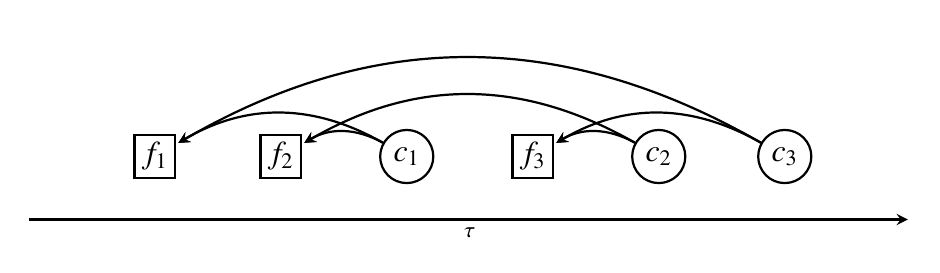
\begin{tikzpicture}[->,>=stealth,shorten >=1pt,auto,node distance=2cm,
                thick,c node/.style={circle,draw,font=\Large\bfseries}, f node/.style={draw,font=\Large\bfseries},scale=0.8, every node/.style={scale=0.8}]


    \draw[->] (-2,-1) to[|->|] node [below] {$\tau$} (12,-1);
    \node[f node] (f1) {$f_1$};
    \node[f node] (f2) [right of=f1] {$f_2$};
    \node[c node] (c1) [right of=f2] {$c_1$};
    \node[f node] (f3) [right of=c1] {$f_3$};
    \node[c node] (c2) [right of=f3] {$c_2$};
    \node[c node] (c3) [right of=c2] {$c_3$};

    \path
    (c1) edge [bend right] (f1);
    \path
    (c1) edge [bend right] (f2);
    \path
    (c2) edge [bend right] (f2);
    \path
    (c2) edge [bend right] (f3);
    \path
    (c3) edge [bend right] (f1);
    \path
    (c3) edge [bend right] (f3);


\end{tikzpicture}
}

\caption{The instance of the lot-sizing problem inducing integrality gap of $4/3$ for LP and the corresponding support of $x$. All drawn arcs correspond to half integral values.}
\label{fig:IGlotsizing}
\end{figure}

Any solution that opens two of the facilities will have a total cost of $2c$ and would be optimal. However, in a fractional solution one can open each facility halfway since each client can be served by two facilities without paying a holding cost, i.e., $y_{f_1} = y_{f_2} = y_{f_3} = 1/2$. See Figure \ref{fig:IGlotsizing} for an illustration. Such a fractional solution satisfies all constraints of LP and has a cost of $3 \frac{c}{2}$, inducing an integrality gap of $\frac{4}{3}$.

\begin{thm}
The natural LP for lot sizing has integrality gap $\ge \frac{4}{3}$.
\end{thm}


\chapter{Resource Sharing in Appointment System}

\section{Introduction}

New York Presbyterian (NYP) Hospital operates a large outpatient MRI service that
consists of three nearby sites within Manhattan, with 7 machines in total.
They provide services, to hundreds of types of scans and they process roughly 100
patients per day. However, patients sometimes experience long waiting time
-about 20\% of all patients wait more than 60 minutes. Futhermore, there are
still unfinished patients at the closing time of a site,
so sometimes the staffs there needs to work a significant amount of overtime. In this chapter,
we discuss a real-time queuing control policy to address these issues,
and a practical implementation to make this feasbile, which takes advantage
of the modern-day reachabilities of patients just prior to their scheduled
appointment.

Patients need to make appointments in advance to reserve their slots.
The slot size, which is of length always an integer multiple of 15 minutes,
depends on the type of scan that the patient is scheduling.
Due to the high demand of MRI services, these machines often have tight
schedules. Together with the high variability in the procedures (which we
shall discuss in details below), these tight schedules cause long waiting times
and substantial overtime to occur.

There are several types of uncertainties that can cause reality to
deviate from the original schedule. There are some Same-Day Add-on Patients (SDAOP)
that will show up without appointments. These are mostly urgent cases
that need to be taken care of. There are also some same-day cancellations.

The most prevalent uncertainty is associated with scan duration and
patient arrival time. MRI scans usually consist of about a dozen of
image series, each with different scanning parameters. If the patient
being scanned moves too much during any series, the images produced
might be too blurred. In this case, the staff will have to redo this series.
Each series can take minutes, so redoing one will lengthen the scan
duration by a non-trivial amount. Futhermore, the scan procedure involves
many human factors. Patients might need extra time to prepare themselves
in the scan bed, and some even experience claustrophobia. Patients may need to
use the restroom during scans. Even the number of images to acquire depends
on the body size of the patients, and varies case by case.

Patient arrival time is another source of uncertainty. Although most
patients arrive on or before their appointment time, some may be
significantly late. This can be caused by bad traffic or the patient
simply leaves home late. Some patients need medical care while being
transported, and they will use Access-A-Ride which provides
such medical care. However, since Access-A-Ride accommodates
multiple patients per day and traffic in Manhattan is unpredictable,
patients might come to their appointments significantly early or late.

The staff usually refers to the situation of running behind schedule
as congestion. When significant congestion happens at one site, the staff there
will call other sites to see whether they can handle more patients. If so,
 they may choose to send patients to other sites using taxi. This practice
may help them balance loads among sites, but it also suffers from several
drawbacks. First, the decision is made solely based on current site status.
Sometimes, the other site is already congested by the time that the transported patient
arrives there. Second, after spending a long time waiting at one site, the patient
needs to be transported to another site. This brings inconvenience to both
patients and staff.

Inspired by their current practice, we developed a real-time queuing control
approach to pool resources across the three sites together. Instead of diverting
patients after congestion develops, we predict when and where congestion will
happen and react by diverting future patients to other sites. Frequently, this
can prevent congestion to happen. Also, since we are diverting future patients
who haven not shown up yet, they can go directly to the other site. This saves
time and effort for both patients and staff. We will describe our approach
in details and show computational results. In fact, our simulation result
based on 3 years of historical data shows that diverting just 3 patients per
day can lead to significant improvement in the number of patients experiencing
very long waiting time staff overtime.

The most closely related literature to our problem is in appointment scheduling.
There are excellent surveys on this topic \cite{gupta2008appointment, cayirli2003outpatient}.
In this setting, usually it is assumed that the health-care providers
already know about patients that must be seen on a particular day,
together with all stochastic characteristics associated with each patient.
The question is to decide the optimal schedule (appointment times of
each patient) to balance patient waiting time, resource idle time and
overtime. Several articles \cite{kaandorp2007optimal,denton2003sequential,begen2011appointment}
have studied this problem and proposed optimal algorithms under
certain assumptions. However, the results are not very applicable
in our case. The reason is that we are working with outpatient facility,
and we cannot really decide appointment times for patients. Nevertheless,
important insights can be drawn from the literature to help make
better schedules.

\section{System dynamics}

In this section, we introduce the dynamics of the system and uncertainty associated with them. There are several type of entities in the system: patients, sites, machines. We are going to discuss each type of entities and how to describe their status in the system. More importantly, we will describe the events corresponding to interaction between these entities. Most of these events are random that they happen randomly or happen at random time. It's important to understand the randomness associated with these events.

\subsection{Entities and states}

\paragraph{Sites} There are multiple sites in our system. Each site also have one or more machines. We assume all machines are homogeneous and are capable of processing any patients. In reality, this is not entirely true, but the difference between machines are quite small so we think the difference can be safely ignored. There is also a single waiting room in each site. Patients who have come but haven't began their scans will stay in waiting room. The time they spend in waiting room is one of the two metrics we are concerned. Sites are scheduled according to open time. If there are unfished patients by end of open time, then the staffs will work overtime. The amount of overtime is another metric in consideration.

\paragraph{Machine} Each machine is located in certain site. Each machine can process one patient at any time, also once a scan is started, it cannot be preempted. For the machine, the status is whether it's currently occupied or not. In addition, if it's occupied, then which patient is under scan and for how long are also tracked in our system.

\paragraph{Appointment} The main way hospital schedule resources allocation is by appointments. Patients usually schedule their appointments about two weeks in advance. At the beginning of the day, we will know the schedule of the day, which will be a list of appointments. Each appointment contains the time, the site and the type of the scan for that appointment. Patient are supposed to go to the site at appointment time. The hospital people can also access various information of the patients like their medical history and the assigned scan protocol by radiologist. Current progress is compared with schedule by practitioners to gauge whether the site is running behind or ahead of the schedule.

Appointments are the central entities in the system. We will track several states of them.
\begin{itemize}
\item Appointment time.
\item Appointment status. This could be "scheduled but patient hasn't shown up", "patient arrived at facility and is waiting", "patient under scan", "scan finished and patient left" or "canceled"
\item Site. This is the site the patient is supposed to go to. We assume patients will go to the site that they're assigned to. If the patient accepts a diversion, then his/her site will change accordingly.
\item Scan type. This is type of scan will be performed on patients. This is determined by the patient's diagnosis need and is decided when the call center schedule for the appointment. Practitioners have working knowledge on estimating duration of scans based on its type. Sometimes, they can have a pretty good estimate on how much congestion may occur based on the schedule and all scan types of that day.
\item Machine used. If patient is under scan, then we will track which machine is used.
\item Arrival time, time when patient finishes preparation before scan, begin time and finish time. We will track progress of appointments. These statistics can help us to figure out what contributes to problems occurred in the system. Whether it's patients arrive too late or scans take too long. In addition, we can make prediction on future based on statistics we collected.
\end{itemize}

\paragraph{Time} Of course, we also need to keep track of current time.


\subsection{Dynamics and Events}

The whole system will evolve throughout the day and states of various entities will change. All of these are driven by events happening throughout the day. We will describe those events that drive the changes and the randomness associated with them.

\paragraph{Patient ready}

This event occurs when patients are ready for scan. After they come to the site assigned when scheduling the appointment, they will first do some preparation for the scan: fill paperworks, change clothes and maybe be put on intravenous therapy (IV). Patients are supposed to be ready at their appointment time, so they actually need to come earlier for preparation. After that, they will be seated at the waiting room until there is available machine to process him/her.

The first uncertainty is that the amount of time needed for preparation is uncertain. Some patients need more help on paperwork or maybe are slow in changing clothes. The second, and more important, uncertainty is their arrival time. Patients come with different transportation options. Some patients come by car. Manhattan is a place where bad traffic is very common. It's not hard to get stuck behind traffic for half a hour. Some patients come by subway or train. This is usually more predictable. However, if the patients are not familiar with these public transportation and, especially, how and where to transfer, then they may need additional time to get through the transportation.

Probably the most unpredictable transportation method is Access-A-Ride. Some patients have medical conditions that require them to have access to medical care throughout transportation. They may resort to Access-A-Ride. These vehicles have medical equipments onboard. However, each vehicle will serve multiple patients per day and appointment is needed. Drivers will optimize the route beforehand according to pickup and dropoff demands. However, if something goes wrong with earlier patients, then delay will propagate onto downstream patients. It's quite common that the driver cannot find a patient at the right time and location due to mis-communication or the car get stuck in traffic. As a result, patients using this service may arrive very early or late.

There is special type of patients called \textit{Same Day Add-on Patient}(SDAOP). They are emergent cases that will simply show up without appointments. We don't a prior know how many SDAOP will show up each day, when will they show up and what type of scans they need to do. Obviously, they will create congestion and all downstream patients will be pushed off.

\paragraph{Appointment cancellation}

Some patients with appointment may cancel their appointment by calling hospital. Their appointments will be removed from schedule. They may reschedule their appointment to another day. This will leave a hole in schedule and may cause machine to idle if no patients are there to fill the gap. But if the site is already running behind, this gap can help it to catch up with schedule and reduce waiting time of downstream patients. However, it's hard to predict who will cancel beforehand.

\paragraph{Scan begin}

Once a machine finish its current patient and become available, the next patient in waiting room will be called in for his/her scan. This is a scan begin event. We're assuming that we prioritize patients according to their appointment time, i.e. people with earlier appointment time will be processed first. This is not entirely true in reality, when a patient comes late and miss their appointment, the hospital may put him/her to wait and process other patients first. The rationale is that they don't want to make patients who haven't done anything wrong to wait. As a result, the late patient may need to wait for long time for a open slot. However, it's not easy to model this behaviour accurately. Thus, we decide to choose a simple and computationally efficient policy that's close enough to reality.

\paragraph{Scan completion} When patients finish their scans, there would be completion event. Patients will check out and leave the system and the machine will become available to process other another patient. The randomness introduced here is the scan duration and this is one of the most important randomness in the system.

There are several reasons why scan duration is highly variable. One most popular scan is BRAIN WITHOUT AND WITH CONTRAST. This involves scan patient's brain for two phases: one without contrast and the other with contrast. After the phase without contrast, a nurse will come to inject contrast via IV so that MRI machine can capture different set of images detailing certain structure in brain. The amount of time to inject contrast is uncertain, although probably not a very stochastic one.

Each type of scan consists of almost ten different image series, each with different parameters and different orientation. If the patient moves too much during any series, the images produced may become very blurred, rendering it useless for diagnosis. In this case, the technologist will have no choice but to redo this series. Each series may take minutes, so redoing one will introduce nontrivial delay to the system.

On top of that, patients may have different body size, which can also influence the amount of images needed to be acquired. Patients may need to go to restroom during the scan, they may be of poor health condition and require other people to help them move onto and off scan table. All these and other factors can affect amount of time the machine is occupied and they together make the scan duration highly variable. Sometimes, patients may experience claustrophobia during scan. The amount of time needed to allow patients to get used to the narrow space inside MRI machines and calm down is uncertain and also highly variable. This will increase duration this patient occupied the resource and add delay to the system.

\subsection{Simulation}

We use simulation to investigate dynamics of the system and evaluate the system performance. Here we describe briefly about our simulation system.

You have already seen in this section that the whole system can be modeled as discrete event system where entities interact with each other through events. We do use discrete event simulation here. However, to be able to do so, we need to have some information about the system in reality so that we can model it in simulation. Fortunately, we have access to data collected by hospital on historical scans done for 3 years. This enables us to conduct simulation in realistic scenarios.

\paragraph{Schedule} We look at the historical schedules and their patterns. We construct schedule accordingly. We know which scans are popular and their proportion among all scans. We also know the slot size allocated for each type of scan.
\paragraph{Uncertainty} Both when patients come and how long their scans take are uncertain. We collect distributions on these information and use them in simulation. Note here we will estimate scan duration for each type of scans.
\paragraph{Unexpected events} From historical data, we can estimate the rate of Same Day Add-on patients and cancellation. We use these rate to randomly generate these unexpected events in simulation.



\section{Resource pooling}

Usually, each day starts with a nice schedule and gradually develops congestions here and there. We have already see why in last section. Here we describe our idea to deal with it as it happens. We mainly want to handle uncertainties that are hard to plan for beforehand, so we decide to take a more reactive approach. This complements good planning and further improves system performance.

As the day evolves, we learn more and more about these uncertainties. For example, maybe several scans at one site took longer than expected or some SDAOP showed up. In either case, that site is probably running behind schedule now. We can balance system loads by moving patients from that congested facility to non-congested facility in real-time. In this way, we can smooth out system unbalance and reduce instability. This helps us improve patient waiting time and reduce site overtime.

\subsection{Why this helps?}

One may concern that by moving patient from congested site A to another site B, we are just moving problems to other place and overall system doesn't run any better. This is definitely legitimate concern, but there are several reasons why diversions can still help.

We are mainly concerned with cases where patients experience extreme long waiting time. By moving patient to non-congested site, we can balance waiting time and overtime among sites thus reduce extreme cases. This in itself is considered beneficial.

Furthermore, by pooling resources, we can alleviate the problem. During daily operation, there are some machine idling time. Appointment cancellation will leave a gap in schedule and machine time may be wasted. If some scan finishes sooner relative to scheduled slot size, the machine time until next patient's appointment may be wasted. If we can somehow leverage these wasted machine time, then patients can generally wait less and sites can incur less overtime. Idle time are more likely to develop at non-congested site since congested ones have to work non-stoping to catch up. By diverting patients from congested site to non-congested one, we will use some machine idle time which will be otherwise wasted. This helps us to process more patients in same amount of time and helps patients to move faster in the system and wait less. This will also help sites to finish the day earlier.

\subsection{Protocol}

There are several issues need to be cleared out before we can implement this idea. All of them are related to the fact that these sites are not collocated. Of course, if all sites are at the same location, all resources are already perfectly pooled together and we won't have any work to do.

\paragraph{Lead time} Patient need some time to prepare to go to a different site.  So we call them about diversion opportunities in advance with respect to their appointment time. Since all sites are close to each other, we think one hour (or 90min) is a reasonable lead time. Suppose a patient has appointment at 3pm. At 2pm, we identified a beneficial diversion. We will call the patient to tell him/her about it. Maybe the patient is still at home so it's relatively easy for him/her to go to a different site. Maybe the patient is on his/her way and, hopefully, it's still easy to change destination. If not, we'll simply ignore this diversion opportunity.

\paragraph{Patient's choice} Of course, we cannot force patient to divert. Our phone call is just offering patients the opportunities to be diverted. Patients can accept or decline the offer. If they decline it, they will still go to their original assigned site. Patients may have some personal stuff to do around the sites before or after their scans. Or maybe their transportation doesn't have flexibility change destination. We will fully respect patient's choice.

\paragraph{Incentive} It's possible that a diversion can benefit overall system, but the patient being diverted doesn't have any benefit or even suffer from longer waiting time. This will create incentive issues and patients won't want to accept such diversions. So when considering diversions, we want to take into consideration the impact on diverted patient and make sure that they experience less waiting time by going to a different site.

\paragraph{No surprise} It's hard for patients to accept diversion if they didn't anticipate it coming. Also, they may be unprepared to receive phone call so they may miss it. Some patients don't even the have the flexibility/interest for diversion. So it doesn't make sense to try to divert patients who don't have the flexibility (for example, patients who use Access-A-Ride for transportation). The night before their appointment day, the hospital people will call them to remind them about the forthcoming scans. At that time, they can also tell patients about potential diversions and ask them whether they want to be volunteers to have the opportunity to go to another site if their original one is very congested. If patients are interested in diversion, then we mark them as volunteers. We will only consider diversions on volunteers. In this way, patients can be better prepared for diversion both physically and mentally. They may watch out for phone call from hospital one hour before their appointment. Also, they may think about ways to go to different sites beforehand. All these can help patients go to a different site more smoothly should opportunities arise.

\section{Policy}

To carry out our idea of resource sharing, we need to figure out among all volunteers, who should we divert and where should we divert them to? It's not as simple as it sounds to just divert patients from congested site to non-congested site. Congestion is a temporal concept: a site is congested in morning doesn't mean it is so in afternoon. We need to define some objective measuring desirability of outcome and, then, we can identify diversions that can improve this objective. Another issue is that because of uncertainties, we don't have a clear-cut answer on whehter a diversion is beneficial or not. It may help or it may hurt. We need make a choice in face of stochastic outcome. Overall, we need to evaluate the impact of diversions with respect to some objective in stochastic setting.

\subsection{Metrics}

Suppose that we are considering some diversion. Without this diversion, the outcome for today will be $\delta$. With this diversion, the outcome will be $\delta'$. $\delta, \delta'$ contains all information we will ever care about (patients' waiting time, sites overtime, patients arrival times, etc). How do we define a objective to guide us toward more desirable outcome?

\paragraph{Waiting time} For sure, we will desire the outcome with less patient waiting time. However, there are many patients. What do we say when one patient is waiting less but the other is waiting more? Let $W(\delta)$ be the vector of waiting time for outcome $\delta$ and define $W(\delta')$ accordingly. Since we are more concerned with the extreme waiting time case, we can use $l2$-norm of $W(\delta), W(\delta')$ to measure how we're doing on waiting time. This will penalize extreme waiting time more. Note that if a patient is ready before his/her appointment, we don't count that waiting.

\paragraph{Overtime} Each site has open time. If the site has to continue operating outside open site, then overtime is incurred. It's usually because there are patients still need processing even after the close time of the site. We like outcome with low overtime. Let $O(\delta), O(\delta')$ be the total overtime over all sites for either outcome. We will put this into our objective. Besides this is a important metric for outcome quality, this also help us to cope with different open time of sites. Suppose one site close at 8pm and another close at 10pm. Then at 9pm, the first site seems pretty empty so we may tempt to divert patient to there. The fact that this will incur a lot of overtime for the first site will prevent us from doing so. Thus, we don't send patient to site that is supposed to be close at that time.

\paragraph{Objective} We can combine $W(\delta), O(\delta)$ into one objective by defining the cost
\[  C(\delta) = \sqrt{n}||W(\delta)||_2 + \lambda O(\delta) \]
Where $n$ is number of patients and $\lambda$ is a parameter controlling
how much weight should we put on overtime when we need to trade off
between patient waiting time and sites overtime.
This will capture both patient waiting time and sites overtime.
By optimizing over this objective, we will favor outcome with low waiting time and overtime.

\paragraph{Waiting time of diverted patient} As we mentioned is last section, we'd like the diverted patient to experience less waiting time for incentive reason. Let $P(\delta), P(\delta')$ be the waiting time of the diverted patient in each outcome.

Overall, a desirable diversion should have two properties. First, we want $P(\delta) > P(\delta')$. In order words, we want the diverted patient to wait less compared to if he/she sticks to the original assigned site. Second, let we want $C(\delta) > C(\delta')$, so system performance is better with diversion.

\subsection{Dealing with stochastic outcome}

At some time of the day, when considering a diversion, we can think about the outcome $\delta, \delta'$ for carrying out the diversion or not. The issue is that both $\delta, \delta'$ are stochastic and we don't know them for sure. Thus, what's the critierion when we say a diversion is good? We decide to consider the probability of improvement. We will say a diversion is \textit{valid} if
\begin{align*}
  \mathbb{P}[C(\delta') < C(\delta)] \ge \theta_c   \\
  \mathbb{P}[P(\delta') < P(\delta)] \ge \theta_p
\end{align*}
where $\theta_c, \theta_p$ are two treshold controlling how aggressive/conservative we are. High threshold ensures we will see improvement for sure, but there may only be very few diversion options.

In other words, the critierion we have is that we want that the overall objective improve with high probability and the patient being diverted experience less waiting time with high probability.

Still we don't know outcomes $\delta, \delta'$, so we can use simulation to sample from the outcome distribution. We just need to find a way to sample all information we don't know yet. Here is the list of information we need and how to sample them.

\begin{itemize}
\item For patients who are under scan, how much more time do they need to finish their scans? We can use historical scan duration distribution and sample from it conditioning on that the scan time is longer than how much time the patient has been under scan.
\item For patients who haven't shown up, when will they show up? Again, we can sample from historical distribution conditioning on the patient hasn't shown up yet.
\item For patients in waiting room or patients who haven't shown up yet, how long will their scans take? We can simply sample from historical scan distribution.
\end{itemize}

Suppose in total generate $k$ sample paths and let $\xi_1, \ldots, \xi_k$ be all the random vectors (all processing time, arrival time, etc information) sampled. Then we can use simulation tool to generate outcomes $\delta(\xi_1), \ldots, \delta(\xi_k)$ for the scenario without current diversion and outcomes $\delta'(\xi_1), \ldots, \delta'(\xi_k)$ for the scenario with current diversion. Now we can compare them by counting for how many $\xi_i$'s that $C(\delta'(\xi_i)) < C(\delta'(\xi_i))$. Here notices we are comparing pair of outcomes using the same random vector. This technique is called \textit{common random numbers}, and this can help us reduce variance. In the end we can use the fraction of pairs where objective improves to approximate the probability that diversion leads to better objective. We use this fraction to compare with the threshold $\theta_c$. We can do the same for waiting time of diverted patient. In this case, we can use simulation to determine which diversions are \textit{approximately valid}. And we will try to carry out these diversions.

\subsection{Making decisions}

Throughout the day, we will try to make a few diversions. For each volunteer, we can try to divert him/her 1 hour before his/her appointment time. We call these times decision epochs. During each decision epoch, we can try all possible diversions for this patient each corresponding to one site, and then look at which subset of them are valid. If there is more than one valid diversion, we will pick the one with the highest probability on objective improvement. The rationale here is that as long as we have enough confidence that diverted patient wait less, then there is enough incentive for the volunteer to accept the diversion, so we should focus on overall system performance.

\paragraph{Remark} When making diversions, we're imagining there is no more diversions afterward. In other words, we're trying diverting patients one by one. There could be better arrangement by diverting several patients at the same time. However, the downside of this is that it's much more complicated. If we want to consider downstream impact of a diversion, we need to model this as stochastic dynamic programming. However this problem has very high dimensional state space so solving it is very impractical. More importantly, it's not easy to coordinate several changes at the same time. The hospital staffs need to call all these patients simultaneously and the deal is sealed only if all of them agree to divert. This may bring significant communication and coordination issues.


\section{Computational Results}

We now present computational results for our diversion policy. Note that
we are omitting confidence intervals for the plots in this section. There
are two reasons for this. First, the plots in this section mostly
contain multiple lines and confidence intervals will substantially clutter
the plots. Second, the number of replications we ran per experiment
leads to confidence intervals of size that do not confirm the statistical
significance of the improvement by our diversion policy. However, because
we used common random numbers across experiments, we are able to confirm
the statistical significance of the improvement by examining the confidence
intervals of the performance improvement (instead of the performance itself).
We include a plot on performance improvement at the end of this section.

\subsection{Experimental Setup}

\paragraph{Scenarios}

In this section, we describe the two scenarios that we experiment with, the historial data we have and choice of parameters of our policy.

The first scenario is based on the real-life case of New York Presbyterian hospital (NYP). NYP hospital has three different sites for outpatients MRI across Manhattan. They are named after their address: York Ave, 55th St and West 84th St. See Figure \ref{fig:site}. The two sites on each side is very close to each other, it's only 15min walking distance. The one on west side is a bit further, it's 15min driving distance without traffic.
Based on this, we think 1 hour lead time is enough for patient to
plan for a different facility.

\begin{figure}
\centering
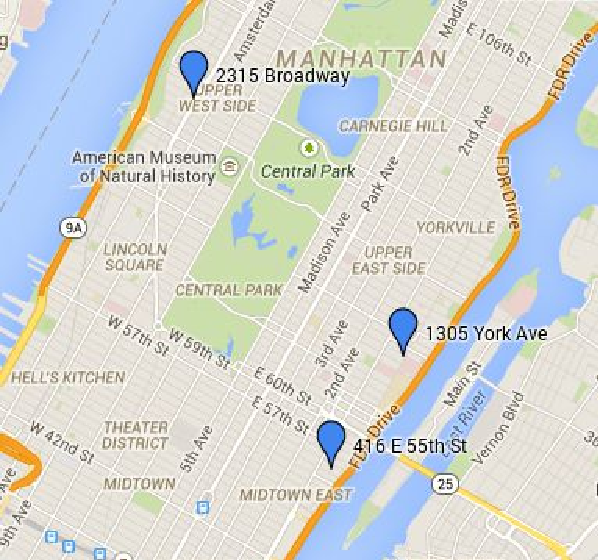
\includegraphics[scale=.6]{chap3/numeric/pic/site.pdf}
\caption{Locations of MRI facilities of New York Presbyterian. There
are three in total represented as blue bubbles. Two of them are on
east side and one is on west side.}
\label{fig:site}
\end{figure}

These sites have different number of MRI machines. West 84th has
only one machine. 55th St has two machines. York Ave has four machines.
Since they have different processing capacity, different number of
appointments are scheduled for. With 4 machines
at York Ave, itself has quite a bit resourcing pooling ability, making
patients there in general wait less.

The second scenario we consider is a system with 7 sites each has one
MRI machine. The reason is that we want to explore the impact of
diversion on a set of small cooperating imaging facilities. Also,
in this case all sites are homogeneous so we can isolate out
the impact of resource pooling without worrying about unbalance in
processing capacities across sites.

\paragraph{Data}

We have three years data of historical MRI scans. For each of these
scans, we have the type of scan, its appointment time, when patient
arrived, when scan began and when scan finished. One thing is missing
here is how much time is needed for patients to prepare before scan.
We overcome this by looking at the first patients processed each day,
and use the difference between their arrival time and scan begin time
as preparation time. Since the first patients don't need to stay in
waiting room, so it's reasonable to assume all time between arrival
and scan begin are used for preparation.

From the historical data, we gathered distribution information on
several things.
\begin{itemize}
\item Scan duration distribution of each type of scan.
\item Patient's arrival time distribution with respect to
their appointment time.
\item The preparation time distribution.
\item Distribution on number of SDAOP showing up in each site.
\item Probability of appointment cancellation.
\end{itemize}
In addition, we also know the slot size allocated for each type of scans.

In our experiments, we generate daily schedules similar to what NYP have in reality.
Then for each appointment, we will sample from the gathered distribution its
scan duration, patient arrival time and patient preparation time. We will also
sample a random variable indicating whether the appointment will be canceled.
In addition, we will also sample SDAOP and their arrival time. With all of these,
we can simulate the operations of a day.

Of course, when our policy is making decision, those sampled random variables
won't be visible. Thus, we can only make decisions based on distributional
information.

Ideally, we'd like to just replay history and test our policy with real
scan duration, arrival time for each historical appointment. However,
the data we obtain isn't perfect. There are some critical fields missing
so we cannot exactly reconstruct history. Also, sometimes, there are
error on timestamps that can greatly impact how the daily schedule looks like.
To prevent these data issues to interfere with our experiments, we choose
to experiment with constructed schedules.

Another thing is that one is one can presumably predict the scan duration and
arrival time better using more information. For example, the patients'
health condition, diagnosis, home address and other information should be
helpful to make better prediction. However, we don't access to those
sensitive health information. But we believe if we can use machine learning
techniques to make better prediction on all the randomness in the system,
our diversion policy will perform better.

\paragraph{Parameters}

There are several parameters we need to choose for setting up our simulation
and for our optimization procedure. We describe our choice of them here.

\begin{itemize}
  \item Volunteer probability. We vary the percent of patients who are willing
    to be volunteer. This will allow us to see the effect of our policy
    with varying level of flexibility.
  \item Lead time. We experiment with both 60min and 90min lead time.
  \item Overtime weight $\lambda = 10$, this reflects the fact overtime is quite valuable.
  \item $\theta_c = 0.7, \theta_p$. We choose the confidence threshold on objective value
    and waiting time of diverted patient to be neither too aggressive nor too conservative.
  \item The number of samples $k=100$.
\end{itemize}

\subsection{3 Sites Results}

We will look at several metrics: waiting time, overtime and number
of diverted volunteers. The reason why we want to look at number of
diverted volunteers is that diversion involves communication and
coordination with patients, so we'd like to achieve improvement
without too much change.

\begin{figure}[htp]
\centering
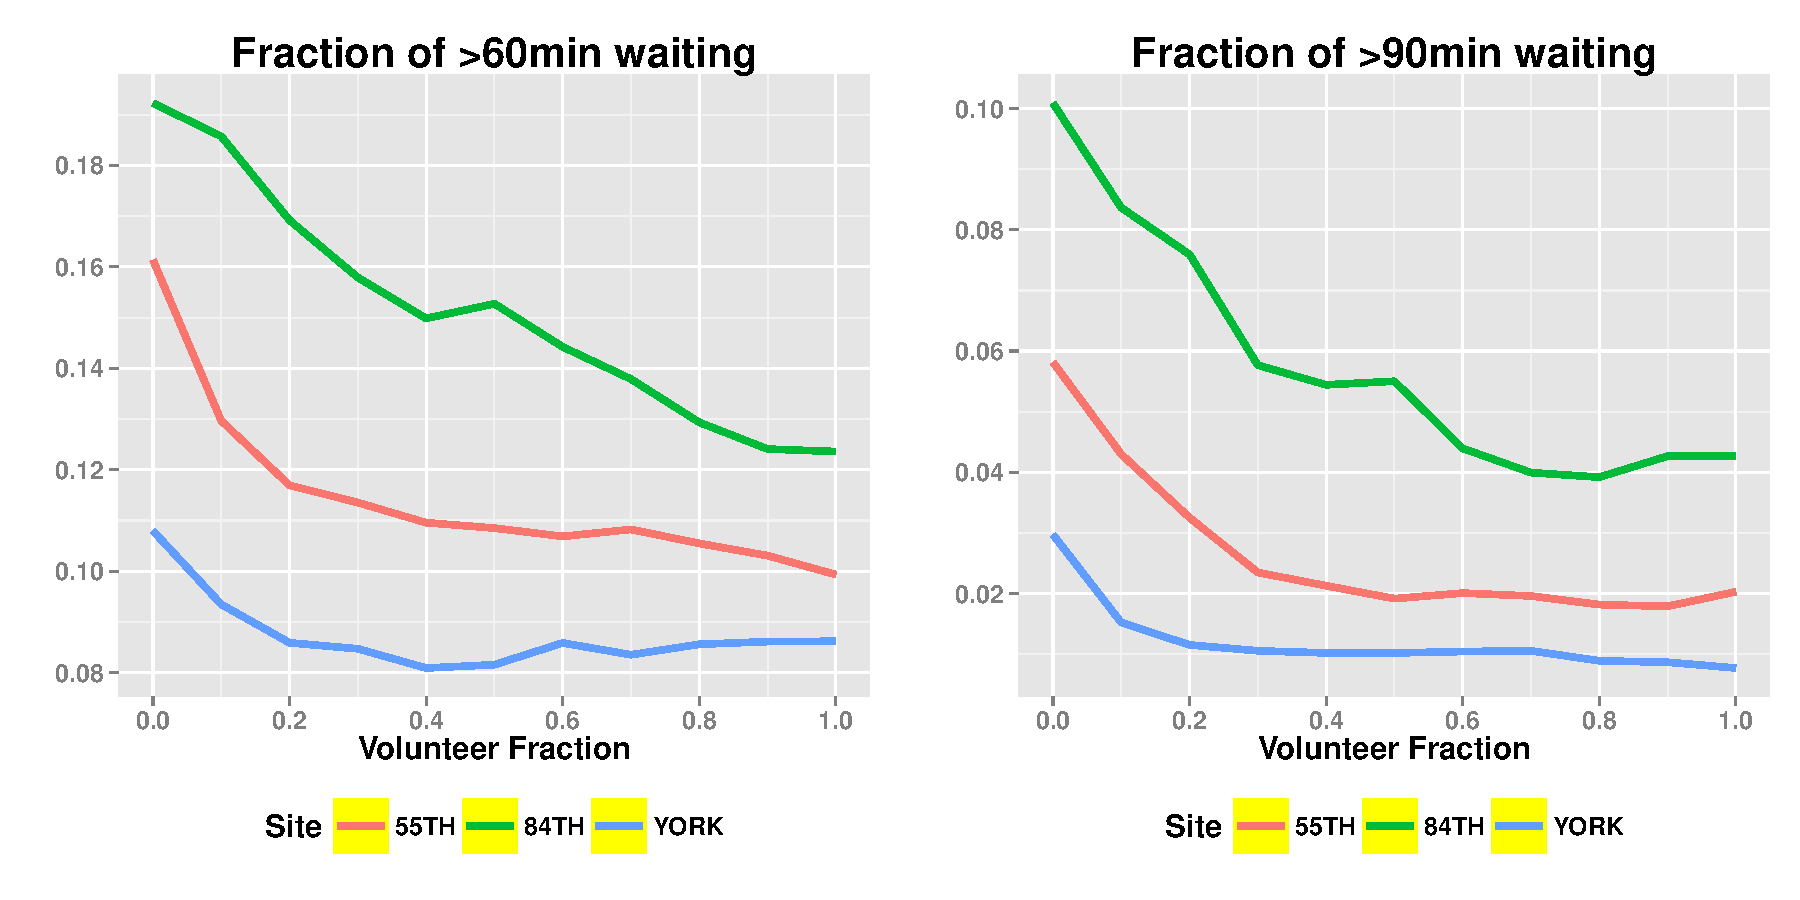
\includegraphics[width=.9\textwidth]{chap3/numeric/pic/3sites_extreme}
\caption{The impact on extreme waiting by diversions. As we increase
fraction of volunteers, we have more flexibility to divert patients,
and we see the extreme waiting cases drop.}
\label{fig:3sites_extreme}
\end{figure}

Figure \ref{fig:3sites_extreme} show how diversion affects extreme waiting times. Without
diversion, about 13.5\% patients wait more than 60min and about
5\% patients wait more than 90min. When we have 40\% patients
as volunteers and 60min lead time, only 10\% patients wait more
than 60min and 2\% patients wait more than 90min.

\begin{figure}[htp]
\centering
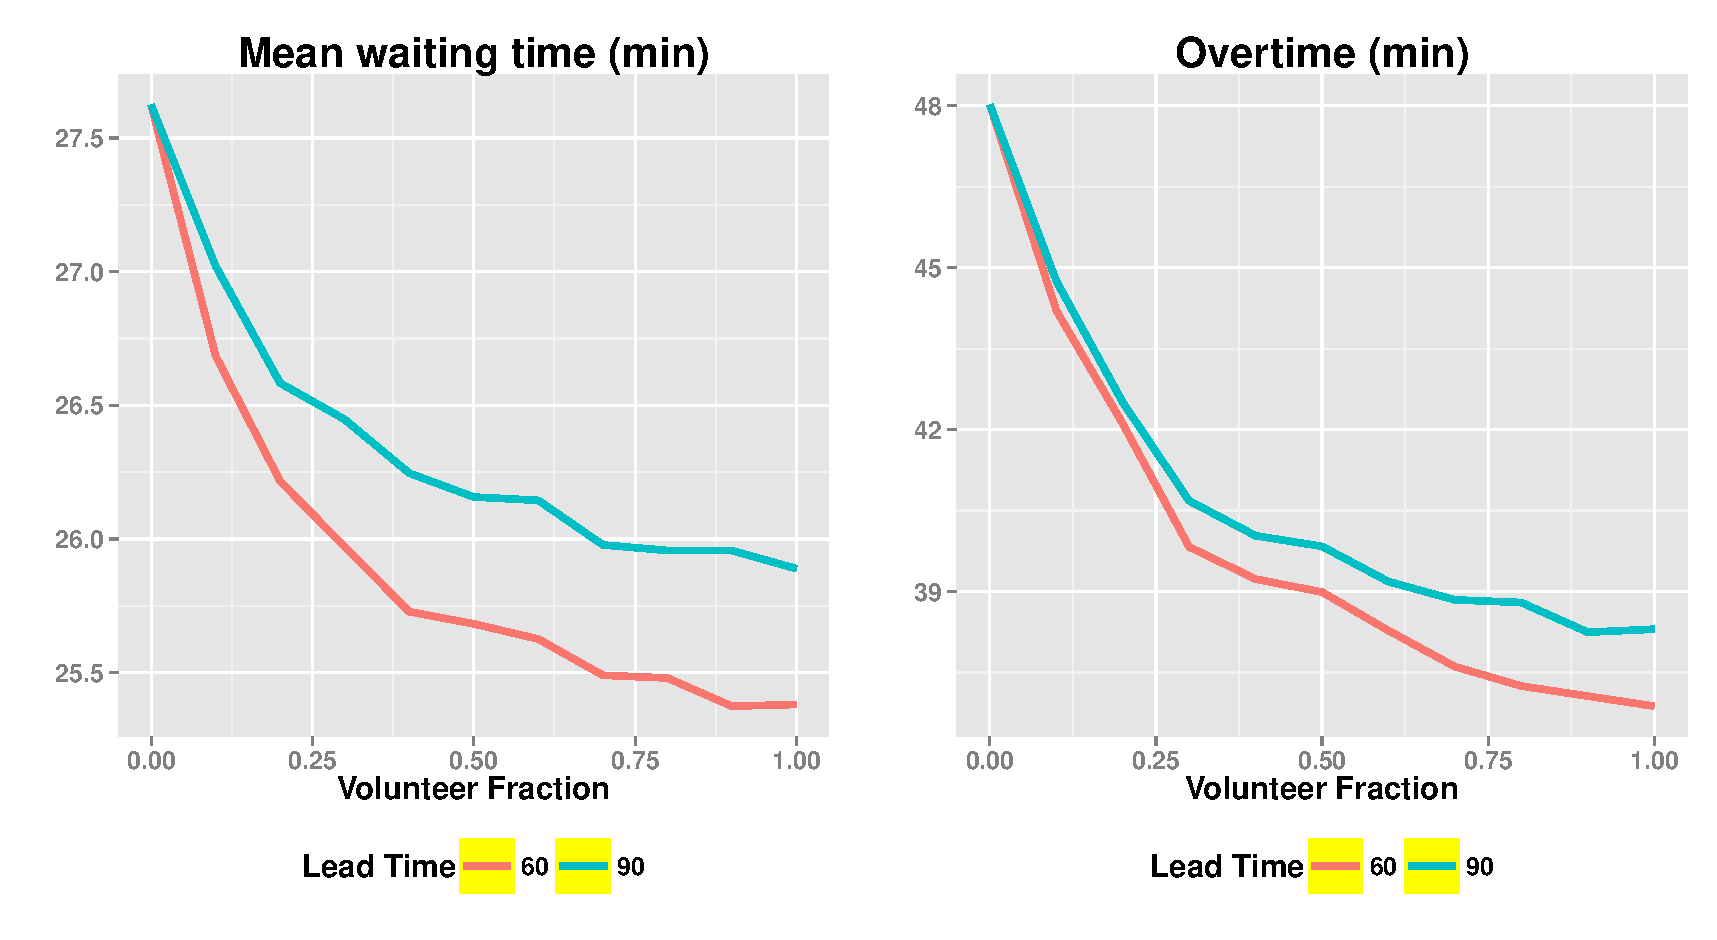
\includegraphics[width=.9\textwidth]{chap3/numeric/pic/3sites_wait_overtime}
\caption{The impact of diversions on mean waiting time and
sites overtime. There is mild improvement on both metric.}
\label{fig:3sites_wait_overtime}
\end{figure}

Figure \ref{fig:3sites_wait_overtime} shows
that we also have mild improvement over mean waiting time of all
patients. Figure \ref{fig:3sites_wait_overtime} shows that with diversion, we also reduce
mean overtime over all sites.

\begin{figure}[htp]
\centering
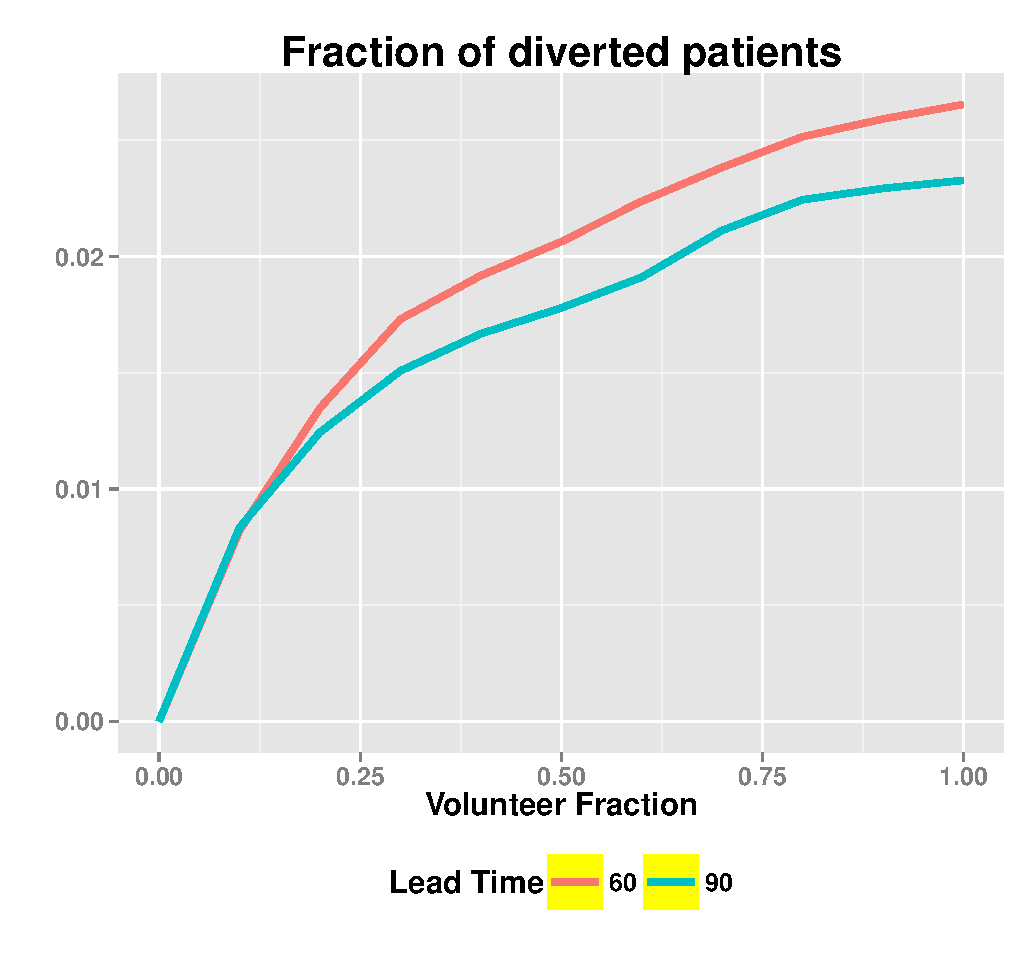
\includegraphics[width=.6\textwidth]{chap3/numeric/pic/3sites_diversion}
\caption{The fraction of patients diverted over all patients.
Only very small fraction of patients are diverted even with
all patients as volunteers.}
\label{fig:3sites_diversion}
\end{figure}

All of these are achieved with diverting
only at most 3\% of all patients as shown in Figure \ref{fig:3sites_diversion}.

\begin{figure}[htp]
\centering
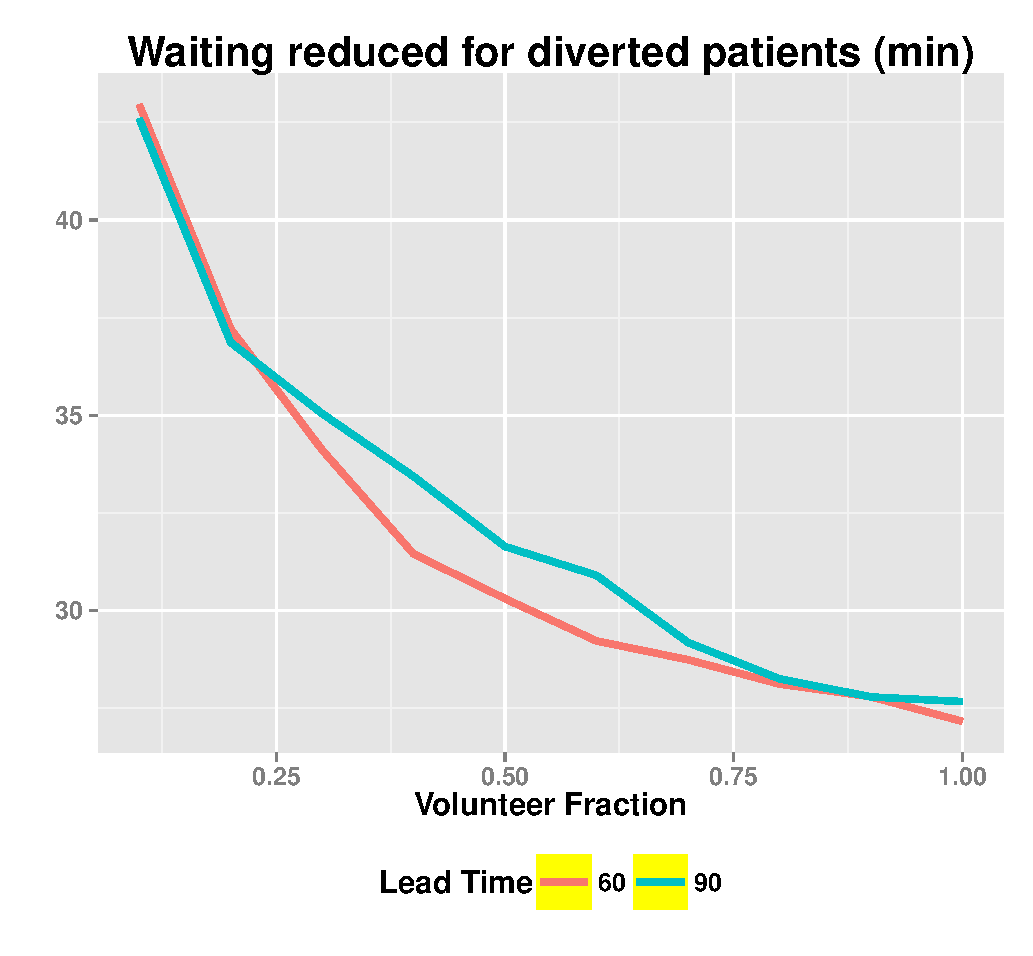
\includegraphics[width=.6\textwidth]{chap3/numeric/pic/3sites_gain}
\caption{Average waiting time reduced for diverted patients.
With more volunteers, the average gain decreases, but it's
still more than 25min with 100\% volunteers.}
\label{fig:3sites_gain}
\end{figure}

Figure \ref{fig:3sites_gain} shows how much waiting
time do the diverted patients save on average. Although it decreases
when we have more volunteers, but still there on average a diverted
patient is expected to wait at least 25min less, which is good incentive
for them to accept diversions. Another thing we can see is that
when we use 90min lead time, we can still achieve most benefits with
60min lead time. This shows that our approach is robust with longer
lead time.

\begin{figure}[htp]
\centering
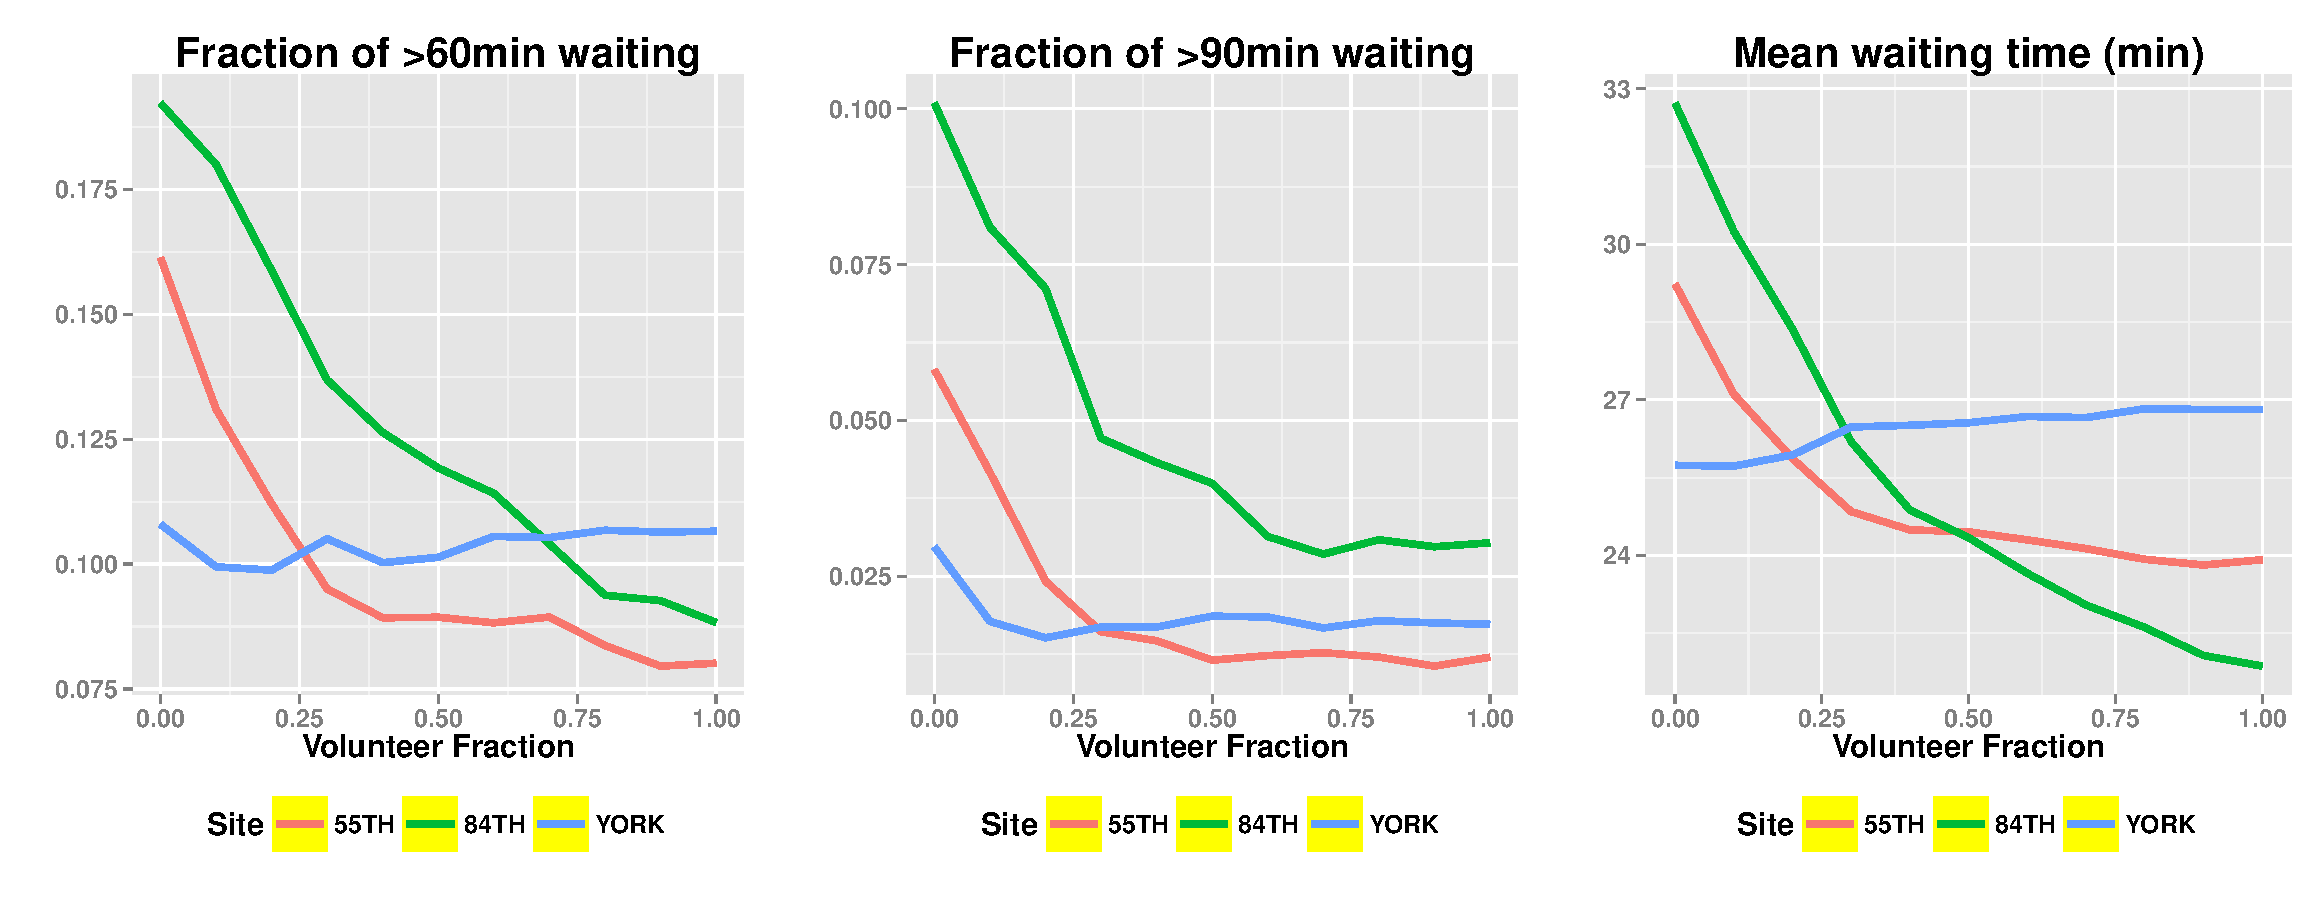
\includegraphics[width=.9\textwidth]{chap3/numeric/pic/3sites_site_wait}
\caption{Impact of diversions on waiting time for each site. It will
greatly improve situations at 55th St and West 84 St, but it will hurt
York Ave a little bit.}
\label{fig:3sites_site_wait}
\end{figure}

\begin{figure}[htp]
\centering
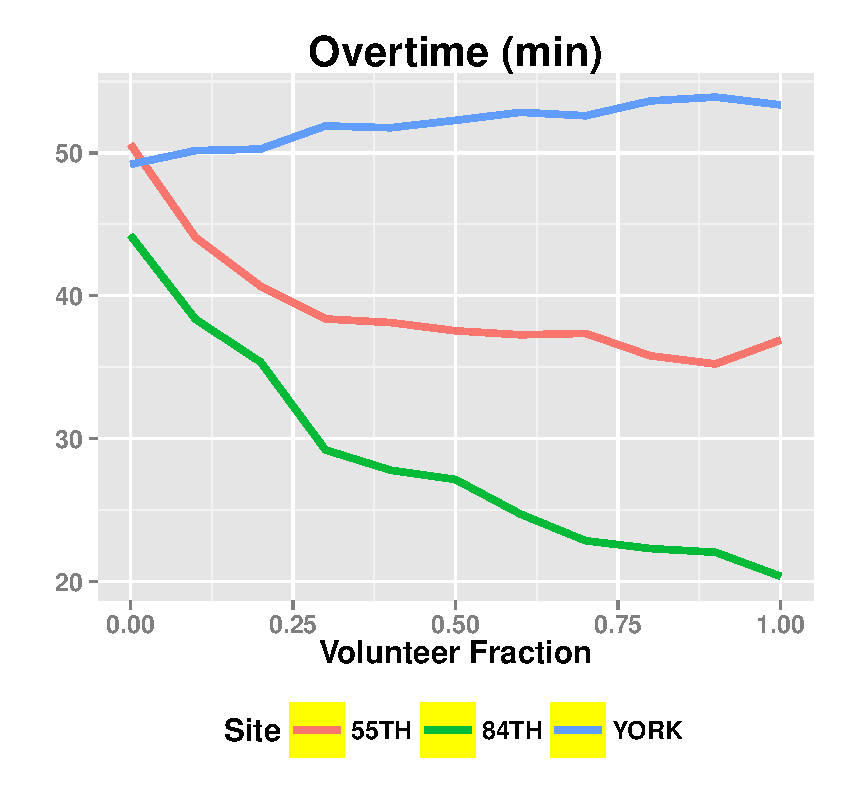
\includegraphics[width=.6\textwidth]{chap3/numeric/pic/3sites_site_overtime}
\caption{Impact of diversions on overtime for each site. Again it will hurt
York Ave a bit, but improves things at 55th St and West 84 St.}
\label{fig:3sites_site_overtime}
\end{figure}

It's also interesting to zoom in and look at what happens at site-level.
Figure \ref{fig:3sites_site_wait} shows the waiting time change per site. Here we see that
although the waiting time for 55th St and West 84th St improves a lot,
it becomes slightly worse. The same is true for overtime, as showed in
Figure \ref{fig:3sites_site_overtime}.

\begin{figure}[htp]
\centering
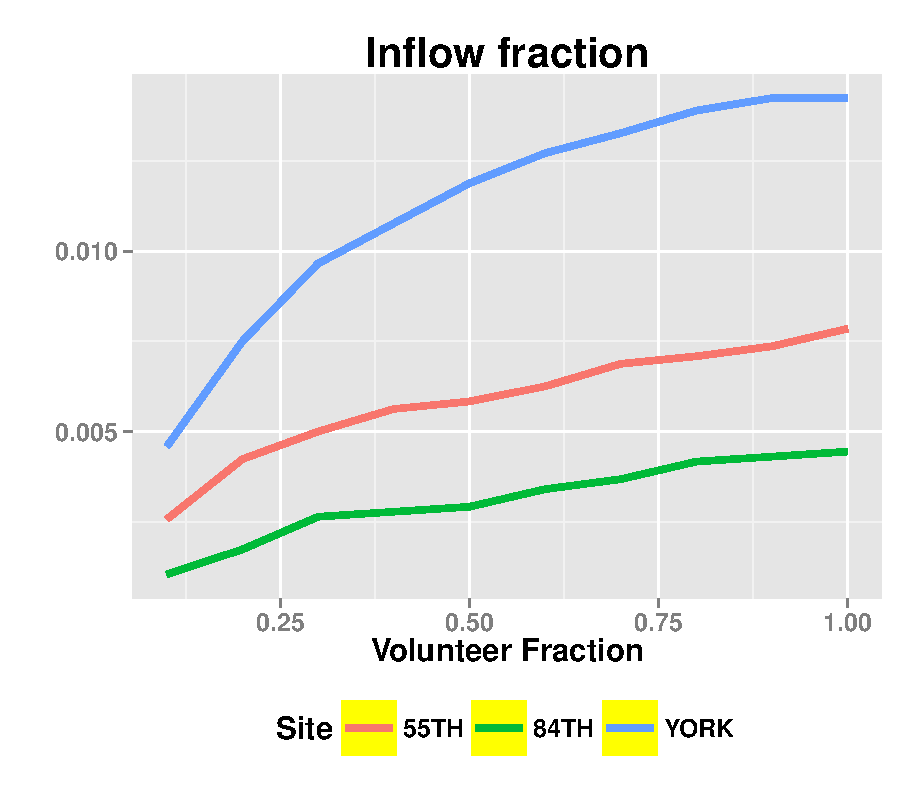
\includegraphics[width=.6\textwidth]{chap3/numeric/pic/3sites_site_inflow}
\caption{Fraction of patients diverted into each site. With four machines,
York Ave becomes the most popular destination and this explains why its
performance got hurt a bit.}
\label{fig:3sites_site_inflow}
\end{figure}

It becomes clear why when we look at Figure
\ref{fig:3sites_site_inflow}. It shows that among all diversions, most are inflow to York Ave.
The reason is that York Ave has 4 machines, so it already gets quite a
bit pooling and thus we're more likely to divert patients there.
However, as we see earlier, the overall performance of the whole
system still improves.

We also did experiment without disruptions like SDAOP or cancellation.
In this case, the system loads are lighter and the system is already
working quite well without diversion. But still, diversions can
produce some small improvement. See Figure \ref{fig:3sites_without_sdaop}.

\begin{figure}[htp]
\centering
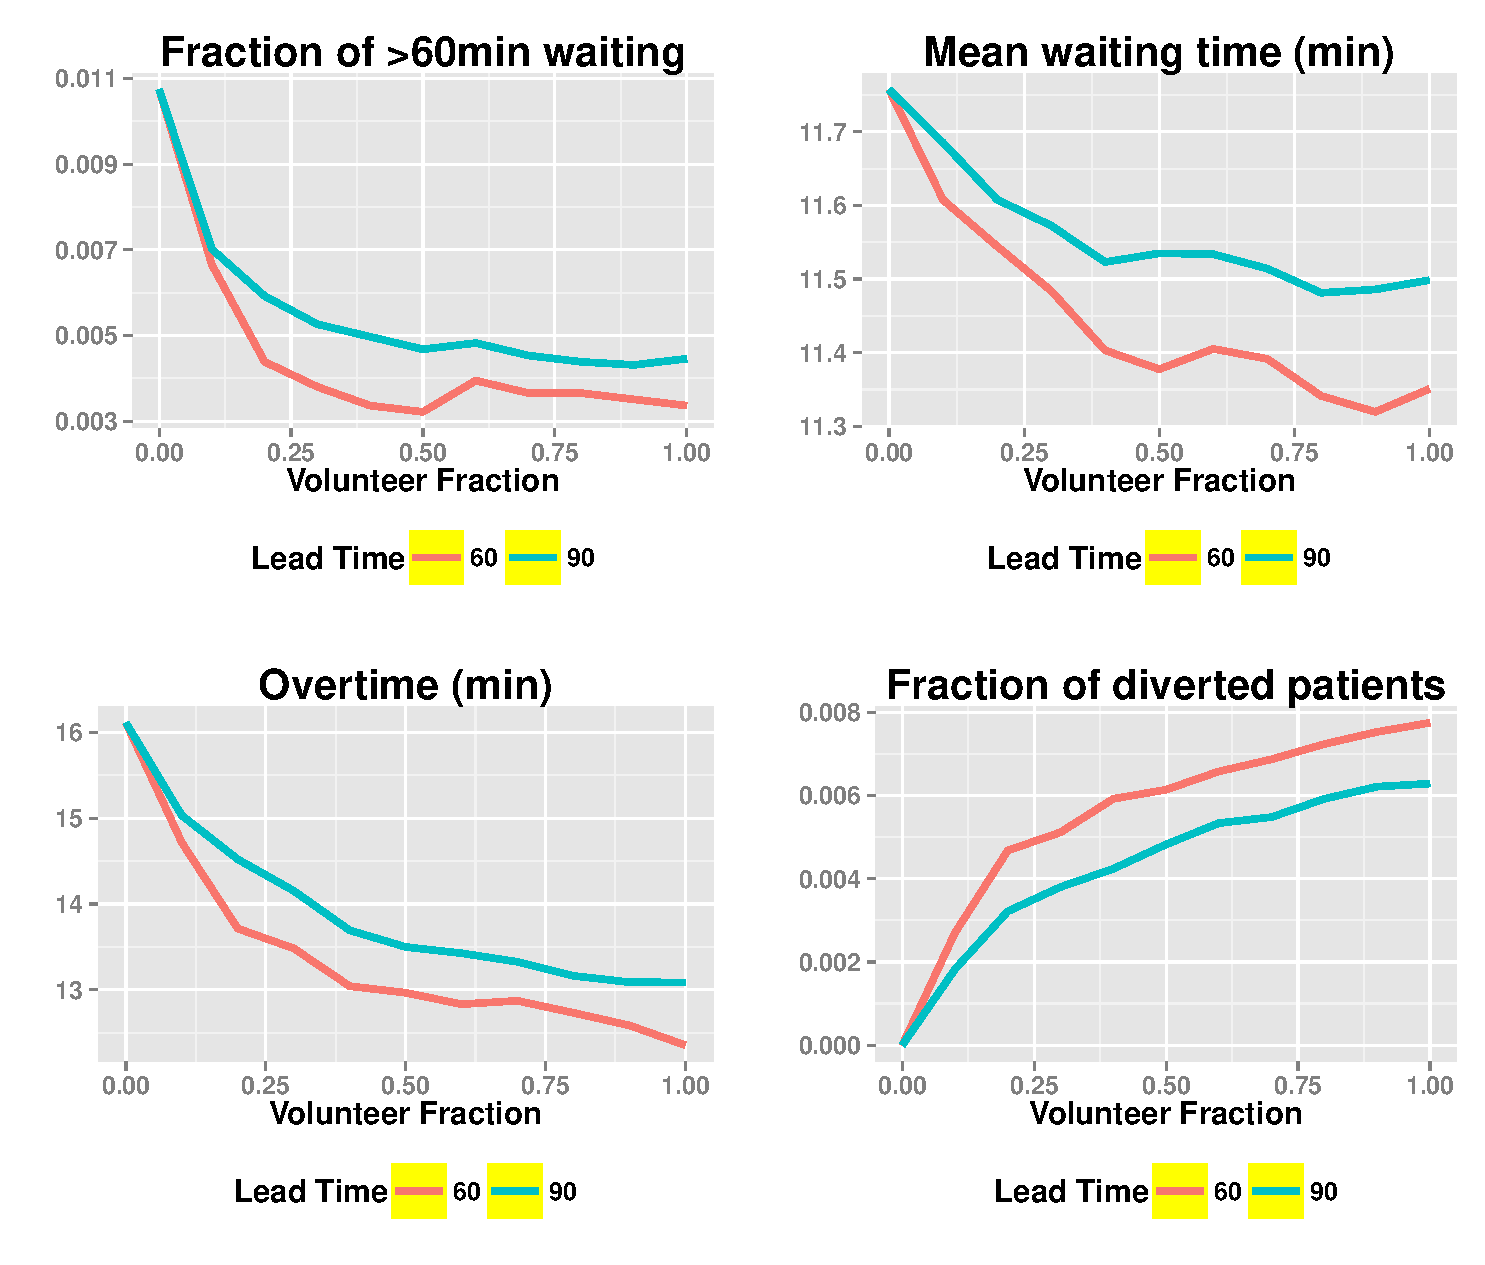
\includegraphics[width=.9\textwidth]{chap3/numeric/pic/3sites_without_sdaop}
\caption{System performance when there is no SDAOP and cancellation.
In this case, the system load is light and there isn't much congestion
to begin with. However, diversions can still achieve some small improvement.}
\label{fig:3sites_without_sdaop}
\end{figure}

\subsection{7 Sites Results}

We'd like to isolate out the impact of simply resource pooling. Thus
it makes sense to conduct experiment on the case where instead of
having some big sites and small sites, we have 7 small sites, each
with one machine. This system has worse performance to begin with
because no pooling effect is present initially. Let's look at the
impact of diversions.

\begin{figure}[htp]
\centering
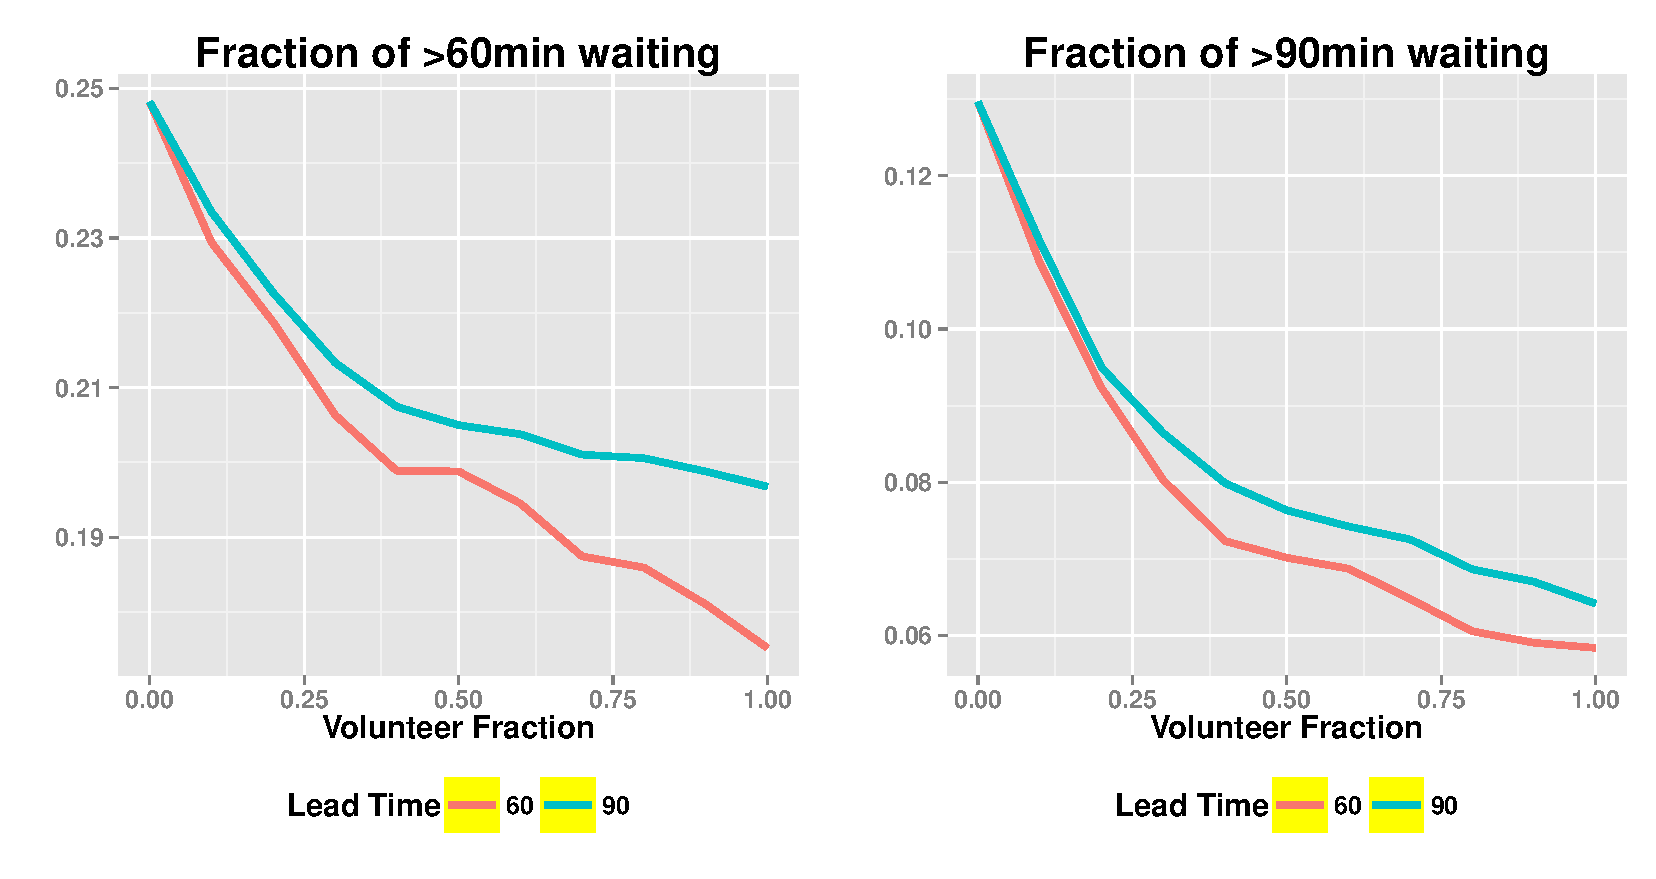
\includegraphics[width=.9\textwidth]{chap3/numeric/pic/7sites_extreme}
\caption{The impact on extreme waiting by diversions. Compare to
3 sites case, we much more significant improvement.}
\label{fig:7sites_extreme}
\end{figure}

\begin{figure}[htp]
\centering
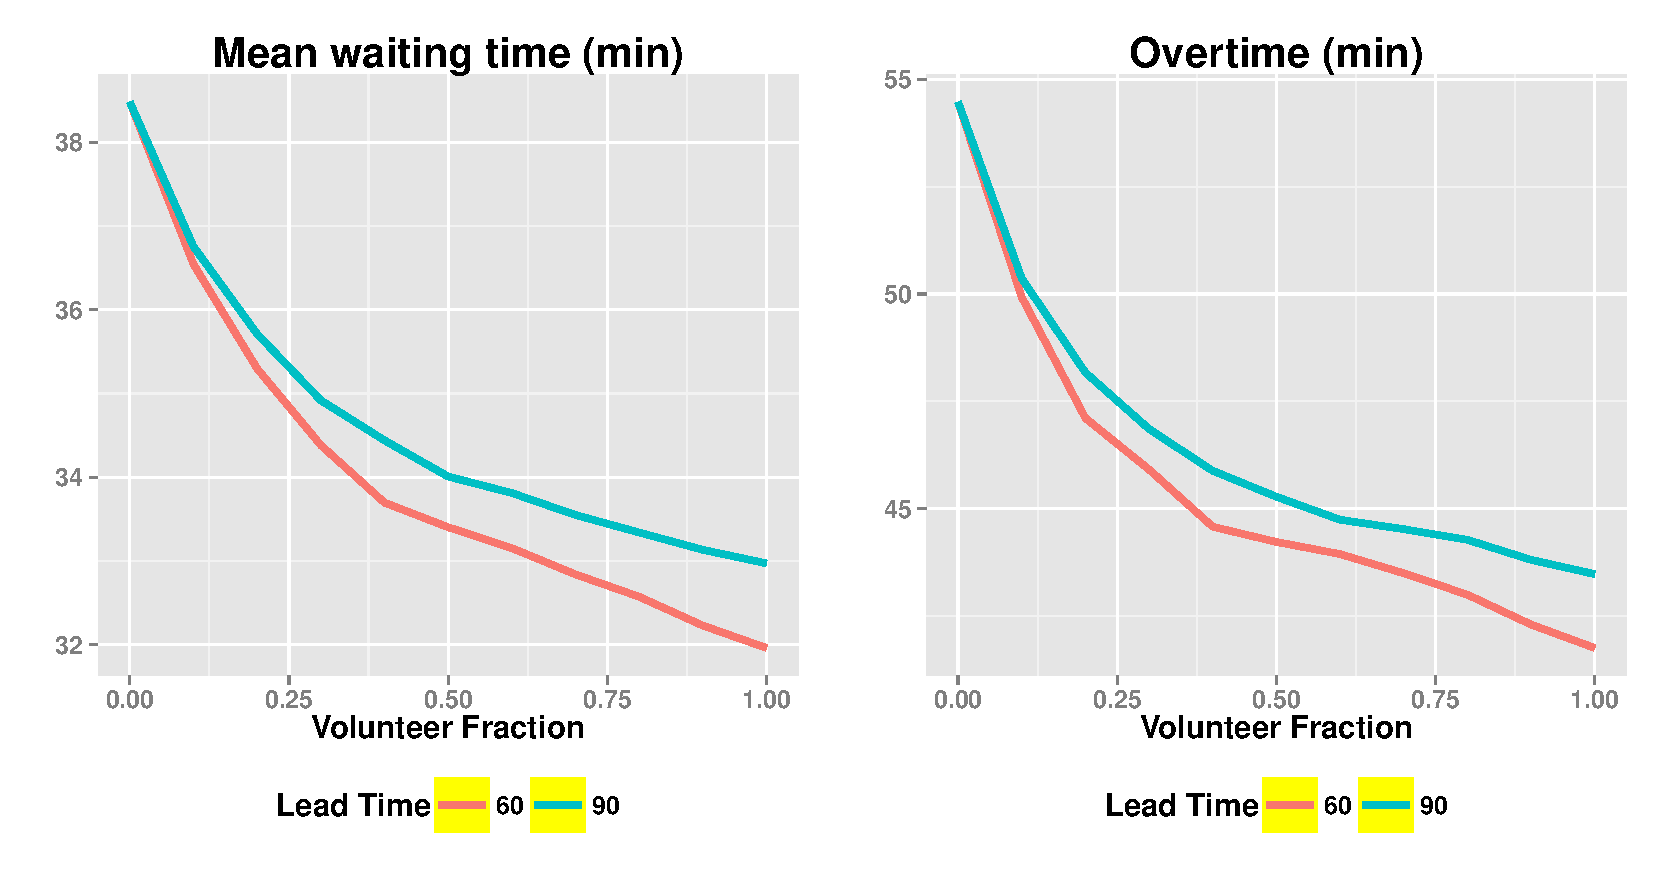
\includegraphics[width=.9\textwidth]{chap3/numeric/pic/7sites_wait_overtime}
\caption{The impact on mean waiting time and overtime by diversions.}
\label{fig:7sites_wait_overtime}
\end{figure}

Figure \ref{fig:7sites_extreme} shows that we have more significant
improvement compared to 3 sites case. This confirmed our intuition
that bigger improvement can be achieved with no pooling effect to begin with.
Figure \ref{fig:7sites_wait_overcome} tells the same story for mean
waiting time and overtime. Note in the end, we can improve mean waiting
time from 38min to 30min, with a 8min difference. And the story is
similar for overtime.

\begin{figure}[htp]
\centering
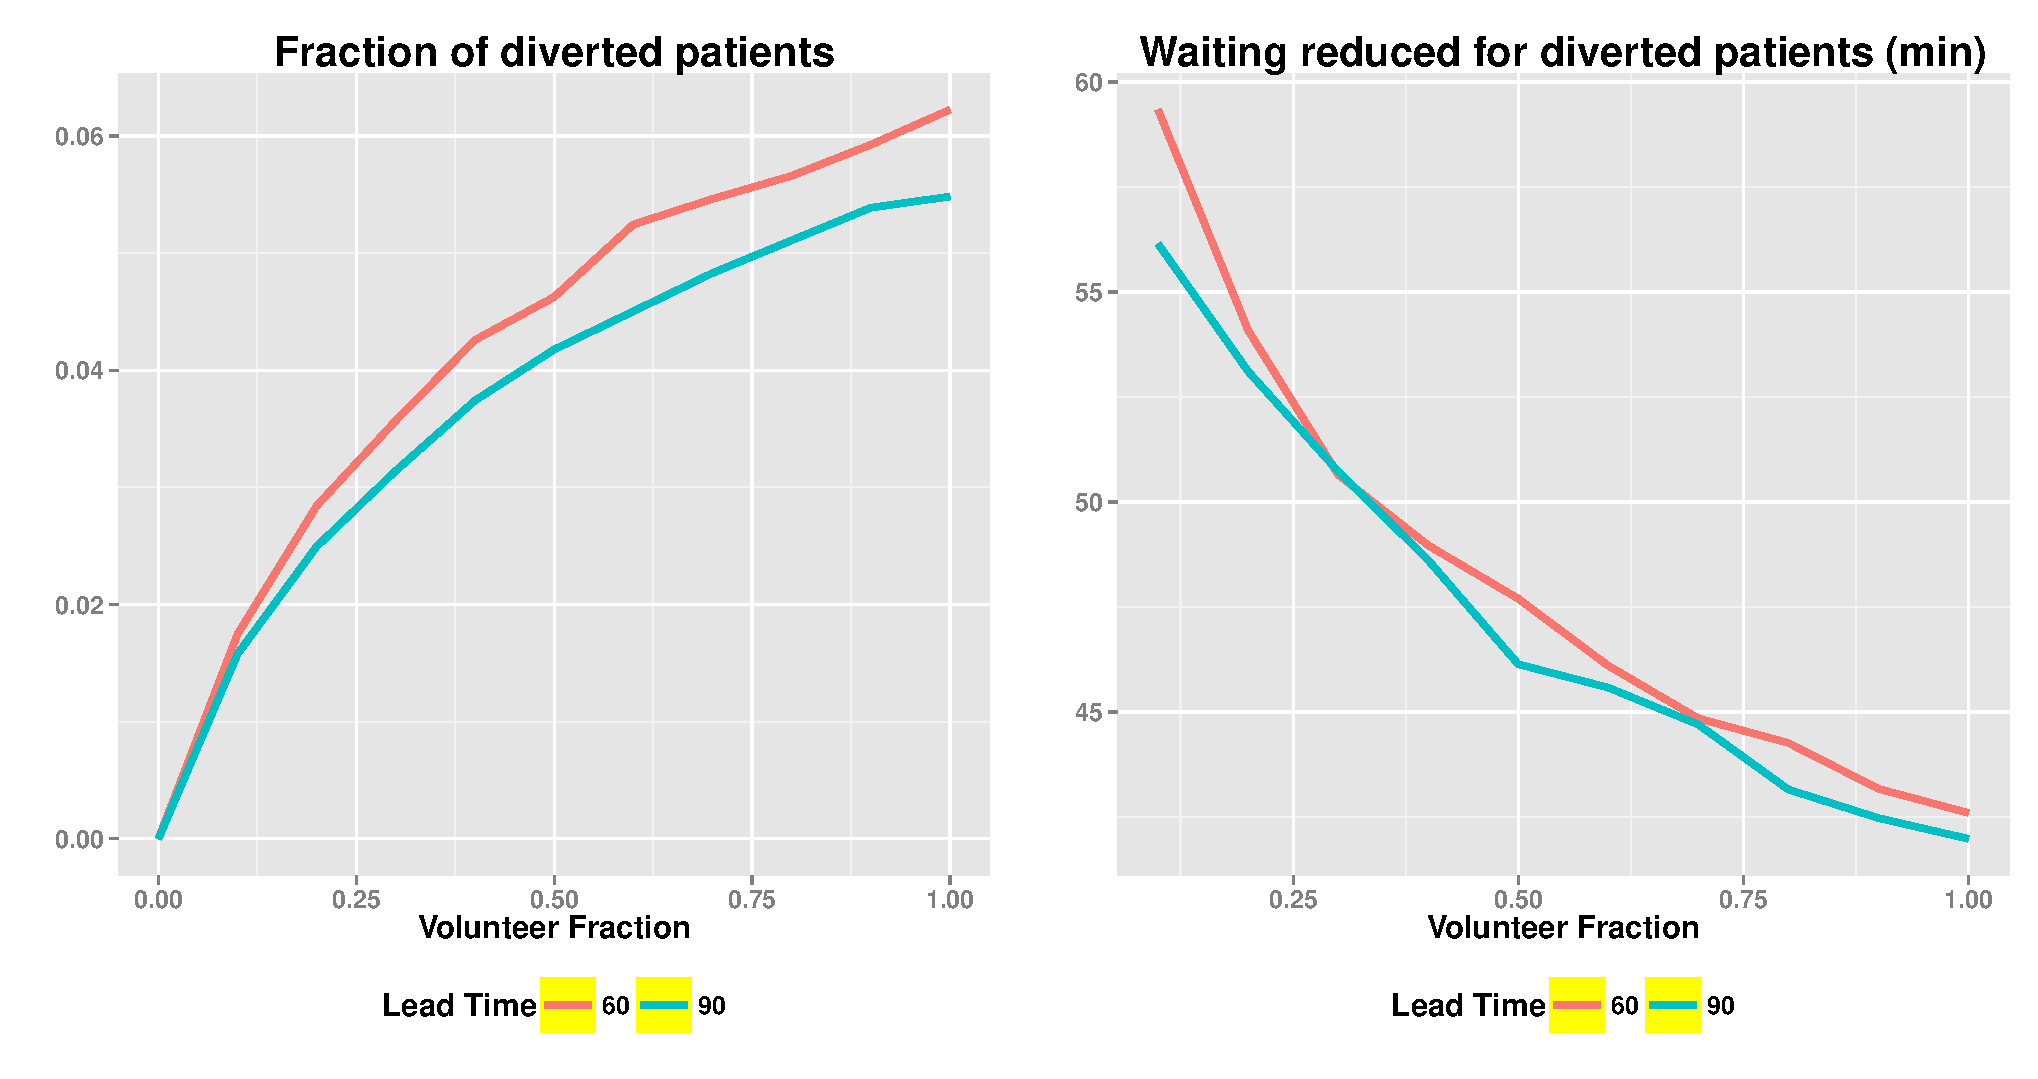
\includegraphics[width=.9\textwidth]{chap3/numeric/pic/7sites_diversion_gain}
\caption{The fraction of diversions and waiting time reduction from diversions.}
\label{fig:7sites_diversion_gain}
\end{figure}

From Figure \ref{fig:7sites_diversion_gain}, we see that we diverted a lot
more patients compared to 3 sites case. With all patients as volunteer, we
diverted more than 6\% of them. This shows that there are a lot more
beneficial diversion opportunities when there is no initially. Also, for
diverted patients, each of them also enjoys more waiting time reduction
compared to 3 sites case.

Note that here all 7 sites are totally homogeneous so there won't be any
unbalance in term of diversion flow and all improvement is equally achieved
by all sites.

Overall, the experiments for the 7 site confirms that greater benefit can
be achieved in the system with many small sites.

\subsection{On confidence intervals}

Figure \ref{fig:ci} details the impact of our diversion policy for the 3 site
case with 60 minute lead time (this is essentially the same
curve for 60 minute lead time as in the first plot of Figure
\ref{fig:3sites_all}). The confidence intervals show that
the positive impact of our diversion policy is statistically
significant. Also, note that as we increase the fraction of
volunteers, the variance also increase. The reason is that,
when there are more volunteers, there are more diversions which
induce more variance. If we examine performance improvment
for other metric or for level of granularity, similar patterns
can be observed.

\begin{figure}[htp]
\centering
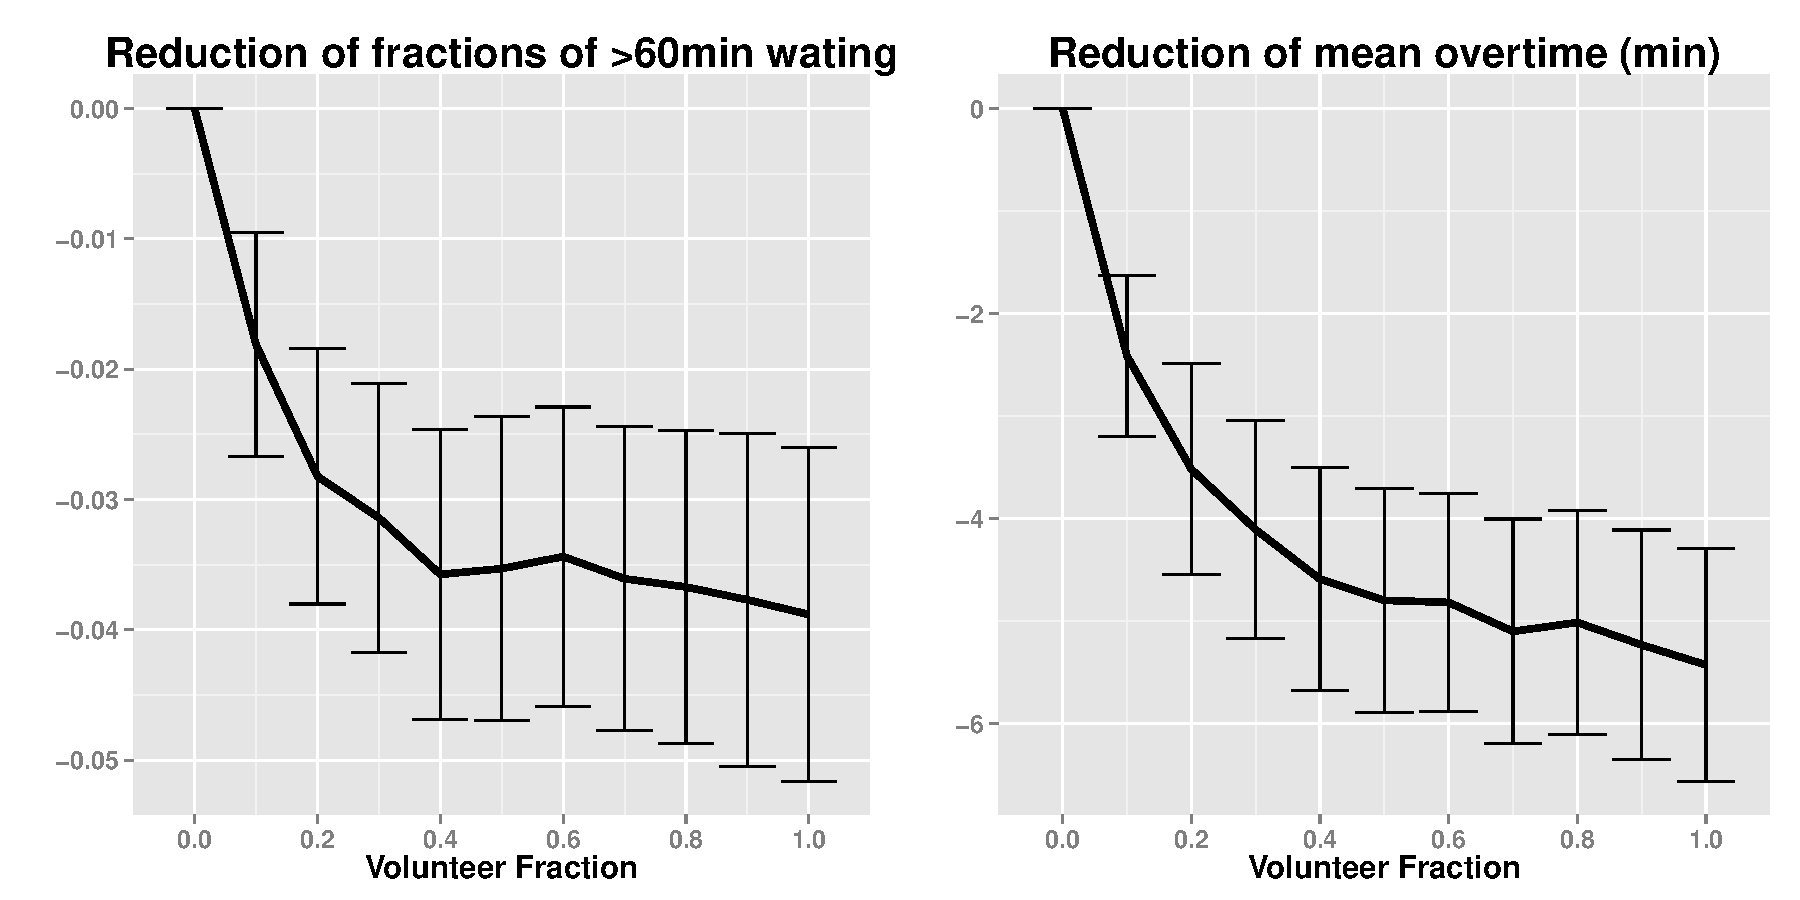
\includegraphics[width=.95\textwidth]{chap3/numeric/pic/ci}
\caption{The improvement on fraction of over 60 minute waiting
for the 3 site case with 60 minute lead time.}
\label{fig:ci}
\end{figure}


% \section{Continuity of system performance with respect to lead time}

In the experiment, we considered two lead times. It is an interesting question
to ask whether the system's performance changes continuously with respect to
the lead time. Here we give a proof for the following similar but simplified setting:
\begin{itemize}
\item There are $k$ sites, each with one machine.
\item There are $n$ patients. Patient $i$ has appointment time $a_i$
      and will arrive punctually.
\item The service duration $d_i$ of patient $i$ follows exponential
      distribution, possibly with different means.
\end{itemize}
For technical reason, we will first slightly modify our instance:
we will use a new appointment time $\tilde a_i = a_i + \delta u_i$,
where $\delta$ is a small constant and each $u_i$ is a uniform
random variable on $[-1,1]$. Now, all of the appointment times
are different almost surely.

The system will follow join-shortest-queue policy with lead time $l$.
Consider the decision epoch at time $\tilde a_i - l$, when the
system is deciding which site to assign patient $i$.
Let $P_{ij}(l)$ be the set of patients that are assigned to site $j$,
but have not completed their scans.
The system will calculate, for each site $j$, the time $C_{ij}(l)$
(at least current time $\tilde a_i - l$) to finish patients $P_{ij}(l)$,
assuming that the scan duration will take expected value. The system
will assign patient $i$ to the site with earliest $C_{ij}(l)$.
If there is a tie, the patient will be assigned to the site with
lower number.

Let sample path $\omega$ includes all of the randomness of $u_i$ and $d_i$,
and let $X(l)$ be the random total waiting time of all of the patients.
We will prove the following theorem.

\begin{thm}
  $\E[X(l)]$ is continuous with respect to lead time $l \ge 0$.
\end{thm}

\begin{proof}
We want to prove $\E[X(l+\epsilon)] \rightarrow \E[X(l)]$ when
$\epsilon \rightarrow 0$.
Number all of the patients from $1$ to $n$ in non-decreasing order of $\tilde a_i$.
Note that the waiting time for any patient $i$ can be bounded
by the sum of scan duration of previous patients $\sum_{i' < i} d_{i'}$.
This implies that the total waiting time $X(l+\epsilon)$
can be bounded by $\sum_{i'=1}^n nd_{i'}$, which is
a integrable random variable. Thus, if we can prove
$X(l+\epsilon) \rightarrow X(l)$ almost surely
as $\epsilon \rightarrow 0$, the theorem will follow from
Dominated Convergence Theorem.

Now fix a sample path $\omega$ and the lead time $l$.
Consider the decision epoch for patient $i$.
Unless there are two sites with empty assigned patients $P_{ij}$, there will almost surely
be a non-zero gap between the earliest completion time $C_{ij}(l)$ and the rest.
Let $g_1>0$ be the smallest such non-zero gap among all of the patients.

Consider the closest pair of decision epoch and moment when a scan
is finished in time, and let $g_2$ be the time between them.
Almost surely, $g_2 > 0$.

We claim that $X(l+\epsilon)=X(l)$, if $|\epsilon| < \min\{g_1, g_2\}$.
Actually, we will prove the two systems will evolve exactly the same.
Suppose that on the contrary, the two systems diverge when
making decisions for patient $i$. Since $|\epsilon| < g_2$,
there is no scan completed between $\tilde a_i -l$ and
$\tilde a_i-\epsilon$, thus $P_{ij}(l) = P_{ij}(l+\epsilon)$ for any site $j$.
In other words, the two systems see the same set of assigned patients.
If there is some site with no assigned patients $P_{ij}(l)$,
both systems will choose such a site with lowest number.
Otherwise, because $|\epsilon| < g_1$, the site with lowest $C_{ij}(l)$
still has lowest $C_{ij}(l+\epsilon)$. The two systems still
make the same decision.

Thus, we have proved that the two system evolve
exactly the same when $\epsilon$ is sufficiently small.
This implies that $X(l+\epsilon) \rightarrow X(l)$ almost surely
when $\epsilon \rightarrow 0$, which completes our proof.
\end{proof}

\section{Conclusion}

In this paper, we look at the problem of congestion in appointment
system with multiple facilities. We explored the approach to make
real-time diversion for resource sharing to balance demands.
We investigate the simple approach of making one diversion at
a time and use simulation and common random numbers to evaluate
proposed changes. This approach is intuitive and simple to
implement. Computational results show that this approach bring
meaningful improvement leading to less patients experiencing
long waiting time with very small number of patients being affected.


%\newcommand{\bV}{{\bm V}}
\newcommand{\Vhat}{\hat{V}}  

\chapter{Mixture logit}

\section{Introduction}

A common problem faced by many firms involves choosing an assortment of products to offer to their customers with the goal of maximizing revenues. There are two sources of difficulty when dealing with such problems. First, the products may serve as substitutes and the customers may make a choice among the products that satisfy their needs. This creates a situation where the demand for each product  depends on what assortment of products are offered to the customers. Second, there can be multiple customer segments served by the firm and the customers belonging to different segments may have different preferences. So, one has to consider the preferences of the different customer segments, as well as the size of each segment, when deciding which assortment of products to offer.


In this paper, we consider an assortment optimization problem to address the difficulties described above.

Each customer makes a choice among the offered products according to the multinomial logit choice model. The crucial feature of our assortment optimization problem is that the parameters of the choice model are assumed to be unknown to the firm and they are modeled as random variables. This type of a situation happens when there are multiple customer segments with different preferences and the segment of a customer is not known to the firm when the customer makes a purchase. The goal of the firm is to choose an assortment of products that maximizes the expected revenue obtained from each customer.

Our work in this paper has connections to the growing literature on assortment planning models in revenue management. In their seminal work, \cite{TalluriVanRyzin:2004} study a version of our assortment optimization problem under the assumption that the parameters of the multinomial logit model are deterministic and known. Under this assumption, the authors show that the optimal assortment includes a certain number of products with the highest revenues. Throughout the paper, we refer to such assortments as revenue-ordered assortments. In this case, the optimal assortment can be obtained efficiently by checking the expected revenue from each assortment that includes a certain number of products with the highest revenues. In contrast, if the  model parameters are random, then \mbox{revenue-ordered} assortments are no longer optimal and the assortment optimization problem appears to be intractable.~Indeed, \cite{BrontMendezVulcano:2009} study the assortment optimization problem with random choice model parameters and establish that the problem is NP-complete when the number of possible realizations of the choice model parameters is at least as large as the number of products.

\paragraph{Our Contributions and Main Results:} The above discussion shows a strong contrast between {\em deterministic} versus {\em random}
model parameters. For the case with deterministic and known  model parameters, knowing the optimality of revenue-ordered assortment has crucial theoretical and practical implications.~On the theoretical side, optimality of revenue-ordered assortments allows us to find an optimal assortment in linear time. On the practical side, optimality of revenue-ordered assortments are intuitively appealing as they urge the firms to shift their focus on high-contribution products, making them easy to justify. Also, optimality of revenue-ordered assortments corresponds to nested protection levels in revenue management settings, where a certain fare class remains open as long as cheaper fare classes remain open. Legacy revenue management systems are commonly tied to the assumption of nested protection levels and using revenue-ordered assortments allow compatibility with such systems.~Our goal in this paper is to close the big chasm between the two cases. Building on the fact that revenue-ordered assortments are optimal when the choice model parameters are deterministic, {\em we investigate the question of what we can say about the performance of such assortments when the choice model parameters are random}.


We focus on the performance of revenue-ordered assortments when the randomness in the choice model parameters does not follow a special structure. If there are~$G$ possible realizations for the choice model parameters and $n$ products that we can possibly offer to the customers, then we show that revenue-ordered assortments provide an approximation guarantee of ~$\min\{G, \lceil n/2 \rceil\}$ (Theorem \ref{thm:guarantee-product}). Furthermore, this performance guarantee is tight in the sense that there are instances of the assortment optimization problem where the expected revenue from the best revenue-ordered assortment deviates from the optimal by a factor of $\min\{G, \lceil n/2 \rceil\}$ (Proposition \ref{pro:tight}).  The tight instances involve products whose revenues differ from each other by orders of magnitude.


\paragraph{Related Literature:} We focus our literature review primarily on papers that use variants of the multinomial logit model to describe the demand process. We refer the reader to \cite{KokFV2006}, \cite{FaJaSh11} and \cite{FaJaSh12} for assortment problems under other choice models.~\cite{TalluriVanRyzin:2004} show that if  customers choose according to the multinomial logit model and the choice model parameters are deterministic and known, then revenue-ordered assortments are optimal.~\cite{GaRa11} show that this problem can directly be formulated and solved as a linear program.~\cite{RoShSh10} study the same problem with a cardinality constraint on the offered assortment and show that although revenue-ordered assortments are no longer optimal, the optimal assortment can be computed efficiently. \cite{JaFa11} also focus on assortment optimization problems where there is a cardinality constraint on the offered assortment. They study the performance of an intuitive pairwise exchange algorithm and show that this algorithm finds the optimal solution when customers choose according to the multinomial logit model with known parameters. \cite{RT:2009} show that revenue-ordered assortments are robust against the uncertainty in model parameters, in the sense that they protect against the worst-case expected revenue. This class of assortments are no longer optimal when the choice model parameters are random. \cite{BrontMendezVulcano:2009} show that the assortment problem is NP-complete in the strong sense under random model parameters, give a mixed integer programming formulation to obtain the optimal assortment and suggest a greedy heuristic. \cite{DiBr11} strengthen the mixed integer programming formulation through valid inequalities. There is some work on solving assortment problems under the nested logit model, which is an extension of the multinomial logit model, allowing correlations between the evaluations of different products by a particular customer. \cite{DavisEtal:2012} give a linear programming formulation of the assortment problem under the nested logit model. \cite{LiRusmevichientong:2012} give a greedy algorithm for the same problem. \cite{GallegoTopaloglu:2012} show how to impose a variety of constraints on the offered assortment when customers chose according to the nested logit model. All of the current work on nested logit model is under the assumption that 
there is a single customer segment with known choice model parameters.


Our work is also related to revenue management models that incorporate customer choice. \cite{TalluriVanRyzin:2004} study a revenue management problem over a single flight leg. Customers choose among the fare classes that are available for purchase and the objective is to adjust the assortment of available fare classes at each period to maximize the total expected revenue. There are a number of papers that extend this work to a flight network; see \cite{GallegoIPD2004}, \cite{LiuV2008}, \cite{KunnumkalTopaloglu:2008}, \cite{ZhangAdelman:2008}, \cite{Talluri:2010}, \cite{GaRa11}, \cite{MeissnerStrauss:2008}, \cite{VoZh12} and \cite{MeSt12}. The fundamental idea in these papers is to formulate various deterministic linear programming approximations. These linear programs have one decision variable for each subset of itinerary products, corresponding to the duration of time during which a subset of itinerary products is made available to customers. As a result, the number of decision variables can get large and it is customary to solve these linear programs by using column generation. The column generation subproblem corresponds to our  assortment problem when customers choose according to the multinomial logit model with random parameters. Of particular interest in this domain is the work by \cite{Talluri:2010} and \cite{MeSt12}, where the authors focus on the case with multiple customer segments and customers from different segments choose according to different choice models. The first paper gives tractable relaxations of the problem when there are multiple segments, whereas the second paper gives valid cuts to tighten the relaxation, but as far as we are aware, it is difficult to a priori characterize the tightness of these relaxations. 


The rest of the paper is organized as follows. In Section \ref{sec:form}, we formulate our assortment optimization problem. In Section \ref{sec:app}, we develop approximation guarantees for revenue-ordered assortments when the randomness in the choice model parameters does not have any special structure.

\section{Model Formulation}
\label{sec:form}

We have $n$ products indexed by $1,2,\ldots,n$, and for each $i$, let $r_i$ be the revenue associated with product $i$.~Without loss of generality, we assume that the products are indexed such that  $r_1 \geq r_2 \geq \ldots \geq r_n$. The customers choose among the offered products according to random utility maximization. In particular, each customer associates the utility
%
%
\begin{align*}
U_i = V_i + \epsilon_i
\end{align*}
%
%
with product $i$, where $\epsilon_i$ is a standard Gumbel random variable with mean zero and we view $V_i$ as the mean utility of product $i$. We normalize the utility of the no purchase option to zero. In this case, if we offer the assortment $S \subseteq \{1,\ldots,n\}$ of products to the customers, then a customer chooses the product with the highest utility if the utility of this product is positive, but otherwise, leaves without purchasing anything. It is a standard result
in discrete choice theory (see, for example, \cite{BenAkivaL1985} and \cite{Tr03}) that if we offer the assortment $S$ to the customers, then a customer chooses product $i \in S$ with probability 
%
%
\begin{align*}
\pi_i(S,\bV) = \frac{e^{V_i}}{1 + \sum_{j \in S} e^{V_j}} \ts ,
\end{align*}
where we use $\bV = (V_1,\ldots,V_n)$ to denote the vector of mean utilities of the products, and make the dependence of $\pi_i(S,\bV)$ on $S$ and $\bV$ explicit. The choice model above is known as the multinomial logit model. If we offer the assortment $S$ and the vector of mean utilities is $\bV$, then the expected revenue obtained from a customer is 
%
%
\begin{align*}
f(S,\bV) = \sum_{i \in S} r_i \ts \pi_i(S,\bV).
\end{align*}
%
%
When the mean utility vector $\bV$ is fixed and known, we can find an assortment that maximizes the expected revenue from a customer by solving the problem $\max_{S \subseteq \{1,\ldots,n\}} f(S,\bV)$. The implicit assumption behind using a fixed mean utility vector is that each customer is probabilistically identical, reacting to an offered assortment in the same manner. On the other hand, if each customer has a different reaction towards an assortment, then the mean utilities that a customer attaches to the products can be modeled as random variables themselves. In that case, we can solve
%
%
\begin{align*}
Z^* = \max_{S \subseteq \{1,\ldots,n\}} \mathbb E \{ f(S,\bV) \}
\tag{\sc Mixture Logit}
\label{eqn:mix}
\end{align*}
%
%
to find an assortment that maximizes the expected revenue over all possible realizations of the mean utility vector. The above expectation  involves the random vector $\bV$ and the distribution of $\bV$ naturally depends on the composition of the market and how customers in the market make a choice.~The random vector $\bV$ can have a discrete or continuous distribution and we assume that it is independent of $(\epsilon_1,\ldots, \epsilon_n)$. We continue referring to $V_i$ as the mean utility of product $i$, although $V_i$ is random.~Throughout the paper, we focus on the \ref{eqn:mix} problem.

The mean utilities $\bV$ can be either discrete or continuous random vectors, depending on the specific application. For example, if we have $G$ customer types, with each type following a multinomial logit choice model, then $\bV$ is a discrete random vector that takes $G$ different values $\hat{\bV}^1,\ldots,\hat{\bV}^G$, where $\hat{\bV}^g$ corresponds to the mean utilities of customer type $g$.  In another example, we can have  $\bV = \bm{\mu} - B \bm{r}$, where $\bm{\mu}= (\mu_1, \ldots, \mu_n)$ is a deterministic vector, $\bm{r} = (r_1, \ldots, r_n)$ gives the prices of the products, and $B$ is a continuous random variable.  In this case, $\bV$ is a continuous random vector, and $B$ is the customer-specific price sensitivity, whose distribution reflects the price sensitivity pattern among the customers.   More generally,
\cite{McTr00} have shown that any choice model based on random utility maximization can be approximated arbitrarily well by the multinomial logit model with random parameters, although the required mixing distribution of $\bV$ can be quite complicated and may be difficult to calibrate.  Thus, the mixture-of-logits model, in principal, can be used as an approximation  in assortment optimization problems under a general choice model.






%with $\Pr\{ \bV = \hat{\bV}^g \} = \alpha^g$ for all $g$.  Then, 
% and $\sum_{g} \alpha^g = 1$. The $g$th possible value of $\bV$ is  $\hat{\bV}^g = (\Vhat_1^g,\ldots, \Vhat_n^g)$ and $\bV$ takes value $\hat{\bV}^g$ with probability $\alpha^g$. We view this situation as serving a market with $G$ customer segments. A customer in segment $g$ has the vector of mean utilities $\hat{\bV}^g = (\Vhat_1^g,\ldots, \Vhat_n^g)$. The relative size of customer segment $g$ is $\alpha^g$, capturing the probability of getting a customer in this segment. The \ref{eqn:mix} problem maximizes the expected revenue over all customer segments.

%In the next two examples, we demonstrate  concrete situations where the \ref{eqn:mix} problem can be of practical interest. The first example corresponds to a case where we serve a market composed of multiple customer segments. The second example corresponds to a case where different customers have different price sensitivities.
%
%
%\begin{example}[Multiple Customer Segments]
%\label{ex:mixture}
%\rm
%Consider the case where the mean utility vector $\bV$ can take $G$ different values $\hat{\bV}^1,\ldots,\hat{\bV}^G$. The $g$th possible value of $\bV$ is  $\hat{\bV}^g = (\Vhat_1^g,\ldots, \Vhat_n^g)$ and $\bV$ takes value $\hat{\bV}^g$ with probability $\alpha^g$. We view this situation as serving a market with $G$ customer segments. A customer in segment $g$ has the vector of mean utilities $\hat{\bV}^g = (\Vhat_1^g,\ldots, \Vhat_n^g)$. The relative size of customer segment $g$ is $\alpha^g$, capturing the probability of getting a customer in this segment. The \ref{eqn:mix} problem maximizes the expected revenue over all customer segments.
%\end{example}
%
%\begin{example}[Customer-Specific Price Sensitivity]
%\rm
%Consider the case where the mean utility of product $i$ is of the form $V_i = \mu_i - B \ts r_i$, where $\mu_i$ is a constant and $B$ is a random variable, so that $\bV = \bm{\mu} - B \bm{r}$ with $\bm{\mu}= (\mu_1, \ldots, \mu_n)$ and $\bm{r} = (r_1, \ldots, r_n)$. We can interpret the random variable $B$ as the customer-specific price sensitivity, whose distribution reflects the price sensitivity pattern among the customers in the market. In this case, the \ref{eqn:mix} problem  finds an assortment that maximizes the expected revenue over all customers with different price sensitivities.
%\end{example}

\section{Performance of Revenue-Ordered Assortments}
\label{sec:app}

In this section, we investigate the performance of revenue-ordered assortments for general instances of the \ref{eqn:mix} problem. Throughout this section, we say that revenue-ordered assortments provide an approximation guarantee of $\beta$ if the expected revenue from the best revenue-ordered assortment deviates from the optimal expected revenue by no more than a factor of $\beta$. In other words, noting that the optimal objective value of the \ref{eqn:mix} problem is denoted by $Z^*$, if we have 
%
%
\begin{align*}
\frac{1}{\beta} \ts Z^* \leq \max_{i =1,\ldots,n} \mathbb E \{ f(\{1,\ldots,i\},\bV)\},
\end{align*}
%
%
for some $\beta \geq 1$, then we say that revenue-ordered assortments provide an approximation guarantee~of~$\beta$.  In the next section, we derive an approximation guarantee that increases linearly with the number of products and customer segments, and prove that it is tight.  This guarantee is applicable when the number of products or customer segments is small. For larger problem instances, we derive other guarantees based on the variations in the mean utilities and product revenues in Section \ref{section:approximation-revenue}.

\subsection{A Tight Guarantee Based on the Number of Products and Customer Segments}
\label{section:approximation-product}

In the next theorem, we show that if there are $G$ possible realizations for the vector of mean utilities and $n$ possible products that we can offer to customers, then revenue-ordered assortments provide an approximation guarantee of $\min\{ G, \lceil n/2 \rceil \}$.

\begin{theorem}[Guarantees Based on Numbers of Mean Utility Realizations and Products]
\label{thm:guarantee-product}
If there are $G$ realizations of the vector of mean utilities, then revenue-ordered assortments provide an approximation guarantee of $\min\{ G, \lceil n/2 \rceil \}$ for the \ref{eqn:mix} problem.
\end{theorem}

The proof of Theorem \ref{thm:guarantee-product} makes use of the following property of the expected revenue function.

\begin{lemma}
\label{lem:app_n}
For every realization of the vector of mean utilities $\bV$, the following two results hold.

\noindent \textup{($i$)} For all assortments $S$ and $T$,  $f(S \cup T ,\bV)\leq f(S,\bV)+ f(T,\bV)$.

\noindent \textup{($ii$)} For all products $i$ and $j$ with $i < j$, $f(\{i,\ldots,j\} ,\bV) \leq f(\{1,\ldots,j\} ,\bV)$. 

\end{lemma}

\begin{proof}
The first result follows immediately from the fact that
$$
f(S \cup T,\bV)
=
\frac{\sum_{i \in S} r_i \ts e^{V_i} + \sum_{i \in T} r_i \ts e^{V_i}}{1 + \sum_{i \in S} e^{V_i} + \sum_{i \in T} e^{V_i}}
\leq
\frac{\sum_{i \in S} r_i \ts e^{V_i} }{1 + \sum_{i \in S} e^{V_i}}
+
\frac{\sum_{i \in T} r_i \ts e^{V_i}}{1 + \sum_{i \in T} e^{V_i}}
= 
f(S,\bV) + f(T,\bV).
$$
To establish the second part of the lemma, note that
$
f(\{i,\ldots,j\} ,\bV)
=
\frac{\sum_{\ell=i}^j r_\ell \ts e^{V_\ell} }{1 + \sum_{\ell=i}^j e^{V_\ell} },
$
which implies that $f(\{i,\ldots,j\} , \bV)$ is a weighted average of $0,r_i,\ldots,r_j$, where the weights associated with each one of these are $1,e^{V_i},\ldots,e^{V_j}$, respectively . By using the same reasoning, $f(\{1,\ldots,j\} , \bV)$ is a weighted average of $0,r_1,\ldots,r_i,\ldots,r_j$, where the weights associated with each one of these are $1,e^{V_1},\ldots, e^{V_i},\ldots,e^{V_j}$, respectively. Since  $r_1 \geq \ldots \geq r_i \geq \ldots \geq r_j \geq 0 $, it follows that  $f(\{1,\ldots,j\} ,\bV) \geq f(\{i,\ldots,j\},\bV)$. %and the second part follows by taking expectations.
\end{proof}

We are now ready to show Theorem \ref{thm:guarantee-product}

\noindent {\bf Proof of Theorem \ref{thm:guarantee-product}}

\begin{proof} 
Let $\hat{\bV}^1,\ldots,\hat{\bV}^G$ denote the possible realizations of the mean utility vector $\bV$.  The first part of the approximation guarantee follows immediately from the fact that for each $g = 1, \ldots, G$,  a revenue-ordered assortment solves the problem 
$\max_{S \subseteq \{1,\ldots,n\}} f(S,\hat{\bV}^g)$, giving us the approximation guarantee of $G$ (see \cite{TalluriVanRyzin:2004}).
To establish the approximation guarantee of $\lceil n/2 \rceil$, let $S^*$ be the optimal solution to the \ref{eqn:mix} problem. We partition the assortment $S^*$ into $k$ assortments $S_1^*,\ldots,S_k^*$ such that each assortment $S_\ell^*$ contains consecutive products. That is, each assortment $S_\ell^*$ is of the form 
%
%
\begin{align*}
\{ i_\ell^*, i_\ell^* + 1, \ldots, j_\ell^*\}
\end{align*}
%
%
for some $i_\ell^*$ and $j_\ell^*$, with $i_\ell^* \leq j_\ell^*$ and  
$$
	i_1^* \leq j_1^* ~<~ i_2^* \leq j_2^* ~<~  \ldots ~<~ i_{k-1}^* \leq j_{k-1}^* ~<~ i_k^* \leq j_k^*.
$$
Although each $S_\ell^*$ may contain a single product with $i_\ell^* = j_\ell^*$, we observe that the number of assortments~$k$ in the partition never has to be greater than $\lceil n /2 \rceil$.  The desired result follows by 
%
%
\begin{align*}
Z^* 
& = \mathbb E \{ f(S^* , \bV )\} 
= 
\mathbb E \{ f(\cup_{\ell=1}^k S_\ell^* , \bV ) \}
\leq 
\sum_{\ell=1}^k \mathbb E \{ f(S_\ell^* , \bV ) \}
=
\sum_{\ell=1}^k \mathbb E \{ f(\{i_\ell^*, \ldots,j_\ell^* \} , \bV) \} 
\\
& \leq
\sum_{\ell=1}^k \mathbb E \{ f(\{1,\ldots,j_\ell^* ,\} , \bV) \} 
\leq
\sum_{\ell=1}^k \max_{i = 1,\ldots,n } \mathbb E \{ f(\{1,\ldots,i\} , \bV ) \}
\leq
\lceil n / 2 \rceil \max_{i=1,\ldots,n} \mathbb E \{ f(\{1,\ldots,i\} , \bV) \},
\end{align*}
%
%
where the first and second inequalities use  the first and second parts of Lemma \ref{lem:app_n}, respectively.
\end{proof}

To see a simple application of Theorem 5.1, consider the case where we serve two customer segments, a price sensitive and a quality sensitive market segment. Price sensitive customers associate the vector of mean utilities $\bm \hat \bV^1 = ( \Vhat_1^1,\ldots, \Vhat_n^1)$ with the products, whereas quality sensitive customers associate the vector of mean utilities  $\bm \hat \bV^2 = ( \Vhat_1^2,\ldots, \Vhat_n^2)$. Theorem \ref{thm:guarantee-product} implies that the expected revenue from the best revenue-ordered assortment is at least half of the optimal expected revenue.

In the next proposition, we show that the approximation guarantee in Theorem \ref{thm:guarantee-product} is tight, so that there are instances of the \ref{eqn:mix} where the expected revenue  from the best revenue-ordered assortment deviates from the optimal by a factor arbitrarily close to $\min\{ G, \lceil n/2 \rceil \}$. 

\begin{prop}[Tight Guarantee]
\label{pro:tight}
There are instances  of the \ref{eqn:mix} problem such that the expected revenue from the best revenue-ordered assortment deviates from the optimal by a factor that is arbitrarily close to $\min\{ G, \lceil n/2 \rceil \}$.
\end{prop}

\begin{proof}
We  construct a problem instance with $G$ possible realizations of the vector of mean utilities and $n = 2 \ts G -1$ products such that the expected revenue from the best revenue-ordered assortment deviates from the optimal by a factor arbitrarily close to $G = \lceil n /2 \rceil$. To simplify the presentation, we give a problem instance with $G=3$ and $n=5$ such that the expected revenue from the best revenue-ordered assortment deviates from the optimal by a factor arbitrarily close to three. Once we give this problem instance, it is easy to see how to generalize this problem instance to an arbitrary $G$. 

We chose $\delta > 0$ and consider the following instance of the \ref{eqn:mix} problem. There are five products. There are three possible realizations of $\bV$, which we denote by $\hat{\bV}^1$, $\hat{\bV}^2$ and $\hat{\bV}^3$. The next table gives the revenues of the products and the values of $\hat{\bV}^1$, $\hat{\bV}^2$ and $\hat{\bV}^3$. Each column in this table corresponds to a product.

\begin{center}
\footnotesize
\begin{tabular}{cccccc}
\hline
Product   & 1 & 2 & 3 & 4 & 5  \\
\hline
Revenues & $\delta$  & $\delta^2$ & $\delta^3$ & $\delta^4$ & $\delta^5$ \\
\hline
$\hat{\bV}^1$ & $- \log \delta$ & $-2  \log \delta$ & $-\infty$ & $-\infty$ & $-\infty$ \\
$\hat{\bV}^2$ & $-\infty$ & $-\infty$ & $- \log \delta$ & $-2  \log \delta$ & $-\infty$ \\
$\hat{\bV}^3$ & $-\infty$ & $-\infty$ & $-\infty$ & $-\infty$ & $- \log \delta$  \\
\hline 
\end{tabular}
\end{center}

\noindent The probabilities of observing the three realizations of the vector of mean utilities are $\delta^4 / (\delta^4 + \delta^2 + 1)$, $\delta^2 / (\delta^4 + \delta^2 + 1)$ and $1 / (\delta^4 + \delta^2 + 1)$. 

The next table gives the expected revenue provided by each possible revenue-ordered assortment and the assortment $\{1,3,5\}$. 



\begin{center}
\footnotesize
\begin{tabular}{cl}
\hline
$S$ & \multicolumn{1}{c}{$\mathbb E \{ f(S,\bV)\}$} \\
\hline
$\{1\}$ &  $\displaystyle \frac{\delta^4}{\delta^4 + \delta^2 + 1} \times \frac{1}{1 + \delta^{-1}}$
\\
$\{1,2\}$ & 
$\displaystyle \frac{\delta^4}{\delta^4 + \delta^2 + 1} \times \frac{2}{1 + \delta^{-1} + \delta^{-2}}$
\\
$\{1,2,3\}$ &
$\displaystyle \frac{\delta^4}{\delta^4 + \delta^2 + 1} \times \frac{2}{1 + \delta^{-1} + \delta^{-2}}
~~+~~
\displaystyle \frac{\delta^2}{\delta^4 + \delta^2 + 1} \times \frac{\delta^2}{1 + \delta^{-1} }
$
\\
$\{1,2,3,4\}$ &
$\displaystyle \frac{\delta^4}{\delta^4 + \delta^2 + 1} \times \frac{2}{1 + \delta^{-1} + \delta^{-2}}
~~+~~
\displaystyle \frac{\delta^2}{\delta^4 + \delta^2 + 1} \times \frac{2 \ts \delta^2}{1 + \delta^{-1} + \delta^{-2}}
$
\\
$\{1,2,3,4,5\}$ &
$\displaystyle \frac{\delta^4}{\delta^4 + \delta^2 + 1} \times \frac{2}{1 + \delta^{-1} + \delta^{-2}}
~~+~~
\displaystyle \frac{\delta^2}{\delta^4 + \delta^2 + 1} \times \frac{2 \ts \delta^2}{1 + \delta^{-1} + \delta^{-2}}
+~~
\displaystyle \frac{1}{\delta^4 + \delta^2 + 1} \times \frac{\delta^4}{1 + \delta^{-1}}
$
\\
$\{1,3,5\}$ &
$\displaystyle \frac{\delta^4}{\delta^4 + \delta^2 + 1} \times \frac{1}{1 + \delta^{-1}}
~~~~~~~~\,~~+~~
\displaystyle \frac{\delta^2}{\delta^4 + \delta^2 + 1} \times \frac{\delta^2}{1 + \delta^{-1}}
~~~~~~~~\,+~~
\displaystyle \frac{1}{\delta^4 + \delta^2 + 1} \times \frac{\delta^4}{1 + \delta^{-1}}
$
\\
\hline
\end{tabular}
\end{center}

\noindent The two terms in the expected revenue from assortment $\{ 1\}$ can be bounded by $\delta^4 / (\delta^4 + \delta^2 + 1) \leq \delta^4$ and $1 / ( 1 + \delta^{-1}) \leq 1 / \delta^{-1}$. Therefore, the expected revenue from assortment $\{1\}$ is bounded by $\delta^5$.~We bound the two terms in the expected revenue from assortment $\{1,2\}$ as $\delta^4 / (\delta^4 + \delta^2 + 1) \leq \delta^4$ and $2 / ( 1 + \delta^{-1} + \delta^{-2}) \leq 2 / \delta^{-2}$, which implies that the expected revenue from assortment $\{1,2\}$ is bounded by $2 \ts \delta^6$. Continuing in the same fashion, the expected revenues from assortments $\{1,2,3\}$, $\{1,2,3,4\}$ and $\{1,2,3,4,5\}$ are bounded by $2 \ts \delta^6 + \delta^5$, $2 \ts \delta^6 + 2 \ts \delta^6$ and $2 \ts \delta^6 + 2 \ts \delta^6 + \delta^5$, respectively. Therefore, the expected revenue from a revenue-ordered assortment never exceeds $4 \ts \delta^6 + \delta^5$. Noting the expected revenue from assortment $\{1,3,5\}$, the ratio between the expected revenue from the optimal assortment and the expected revenue from the best revenue-ordered assortment is at least 
%
%
\begin{multline*}
\frac{
\frac{\delta^4}{\delta^4 + \delta^2 + 1} \times \frac{1}{1 + \delta^{-1}}
+
\frac{\delta^2}{\delta^4 + \delta^2 + 1} \times \frac{\delta^2}{1 + \delta^{-1}}
+
\frac{1}{\delta^4 + \delta^2 + 1} \times \frac{\delta^4}{1 + \delta^{-1}}
}
{4 \ts \delta^6 + \delta^5}
\\
=
\frac{
\frac{1}{\delta^4 + \delta^2 + 1} \times \frac{\delta^{-1}}{1 + \delta^{-1}}
+
\frac{1}{\delta^4 + \delta^2 + 1} \times \frac{\delta^{-1}}{1 + \delta^{-1}}
+
\frac{1}{\delta^4 + \delta^2 + 1} \times \frac{\delta^{-1}}{1 + \delta^{-1}}
}
{4 \ts \delta + 1},
\end{multline*}
which can be made arbitrarily close to three by choosing $\delta$ small enough.
\end{proof}

%\chapter{Other results}
\section{Compute optimal distribution}

Consider the following problem.
\begin{align}
\max_{F} \quad & \E_{X \sim F} X^+ \\
\text{s.t.} \quad & \E_{X \sim F} X = 0    \\
& \Var_{X \sim F} X = 1
\end{align}
That we want to find, among all distribution with mean $0$ and variance $1$, the distribution with maximum expectation over positive part.
How do you solve this problem?

We can rewrite this problem as a Linear Programming
\begin{align}
\max \quad & \int_0^\infty t x(t) dt    \\
\text{s.t.} \quad & \int x(t) dt = 1    \\
& \int t x(t) dt = 0    \\
& \int t^2 x(t) dt = 1  \\
& x(t) \ge 0
\end{align}
Here $x(t)$ is the pdf of distribution we want to optimize.
This is a Linear Programming with uncountable number of variables.

Take the dual, we get
\begin{align}
\min \quad & y_0 + y_2  \\
\text{s.t.} \quad & y_0 + ty_1 + t^2y_2 \ge t \quad \forall t \ge 0 \label{cons:quad} \\
& y_0 + ty_1 + t^2y_2 \ge 0 \quad \forall t \le 0 \label{cons:quad2}
\end{align}
This Linear Programming has only three variables, but has infinite number of constraints.
However, this is more tractable than the primal and it's possible to derive solution
with extensive and boring computation of case analysis.

We take a different route. Now let's focus on constraints (\ref{cons:quad}).
We can rewrite this as
\[  \min_{t \ge 0} \, y_0 + t(y_1 - 1) + t^2y_2 \ge 0  \]
For the minimization problem, the Lagrangian dual problem is
\[  \max_{\alpha \ge 0} \, \min_t \, y_0 + t(y_1 - 1) + t^2 y_2 - t \alpha    \]
Since $t$ is unconstrained now, we can easily solve the inner minimization problem
\begin{align}
 & \min_t \, y_0 + t(y_1 - 1) + t^2 y_2 - t \alpha   \\
=& \min_t \, y_2(t - \frac{\alpha + 1 - y_1}{2y_2})^2 + y_0 - \frac{(\alpha + 1 - y_1)^2}{4y_2} \\
=& y_0 - \frac{(\alpha + 1 - y_1)^2}{4y_2}
\end{align}

As a result, we have turned constraints (\ref{cons:quad}) into
\[  \max_{\alpha \ge 0} \, y_0 - \frac{(\alpha + 1 - y_1)^2}{4y_2} \ge 0    \]
It's easy to show that $y_0 \ge 0, y_2 \ge 0$, thus, this is equivalent to
\[  \max_{\alpha \ge 0} \, 4 y_0 y_2 \ge (\alpha + 1 - y_1)^2    \]
Note this is a rotated second order conic constraint.
We can do the same to constraints (\ref{cons:quad2}), and get
\[  \max_{\beta \ge 0} \, 4 y_0 y_2 \ge (y_1 + \beta)^2    \]

Now we can rewrite our original problem as
\begin{align}
\min \quad & y_0 + y_2   \\
\text{s.t.} \quad & 4 y_0 y_2 \ge (\alpha + 1 - y_1)^2 \\
& 4 y_0 y_2 \ge (y_1 + \beta)^2 \\
& y_0, y_2, \alpha, \beta \ge 0
\end{align}
This is a second order conic programming and can be efficiently solved.
The optimal solution is actually a pretty simple distribution: it takes $-1$ and $1$ with half probability.

In general, we can solve the following problem
\begin{align}
\max_{F} \quad & \E_{X \sim F} f(X) \\
\text{s.t.} \quad & \E_{X \sim F} X = \mu    \\
& \Var_{X \sim F} X = \sigma^2
\end{align}
where $f$ is a piecewise linear function and
\[ f(x) = c_ix + d_i \quad a_i \le x \le b_i    \]
If you carry out the derivation similar to what we just did,
you will reach the following programming,
\begin{align}
\min \quad & y_0 + y_2  \\
\text{s.t.} \quad & 4(y_0 - d_i + a_i \alpha_i - b_i \beta_i) y_2 \ge (y_1 - c_i - \alpha_i + \beta_i)^2 \quad \forall i    \\
& y_0 - d_i + a_i \alpha_i - b_i \beta_i \ge 0  \quad \forall i \\
& y_2, \alpha_i, \beta_i \ge 0
\end{align}
\section{Another primal-dual algorithm for Joint Replenishment Problem}

\subsection{Preliminaries}
Joint replenishment problem is a well-studied problem in operations research community. Here we consider the deterministic version. Let's formally define the problem. There are $N$ item types numbered $1,2,\ldots,N$. And our whole planning horizon is discrete time $1,2,\ldots, T$. There are a set of demands and each demand is a pair $(i,t)$ where $i$ is the item type of the demand and $t$ is the time when this demand arrives. To satisfy demands, we place orders during our planning horizon. If we make a order consisting of items $S$ at time $s$, it will costs $K_0+\sum_{i\in S} K_i$, and can be used to satisfy demand $(i,t)$ arrives no later than $s$ and $i \in S$, notice here the cost of order doesn't depends on demands quantity of each item type satisfied. To balance the ordering cost, we also have delay cost. If a demand $(i,t)$ is satisfied at some later time $s$, then it incurs delay cost $w_{its}$. The only assumption we have about $w_{its}$ is that it's nondecreasing with respect to $s$. The objective is to satisfy all demands with minimum sum of ordering cost and delay cost.

The main result of this paper is the following
\begin{theorem}
There exists a primal dual 2-approximation algorithm without pruning stage for Joint Replenishment Problem.
\end{theorem}

\subsection{LP formulation}
We start by formulate the primal and dual LP of this problem, let $C(S) = K_0 + \sum_i K_i$ be the ordering cost of set of items $S$ and $\Delta_{its} = w_{it,s+1} - w_{its}$ be the incremental delaying cost, then the primal LP is
\begin{align}
	\min \quad & \sum C(S) x(S,t) + \sum \Delta_{its}z(i,t,s) \\
	s.t \quad& \sum_{S \ni i} \sum_{r=t}^s x(S,r) + z(i,t,s) \ge 1
\end{align}
Here we use $x(S,t)$ to denote whether we put a order of set $S$ at time $t$, $z(i,t,s)$ indicate whether demand $(i,t)$ need to wait from time $s$ to $s+1$. The constraint says that if there is no ordering containing $i$ from time $t$ to $s$(inclusive), then demand $(i,t)$ need to incur the incremental delay cost $\Delta_{its}$.

The dual provides a different view of this problem in term of budget
\begin{align}
	\max \quad & \sum y(i,t,s) \\
	s.t \quad & y(i,t,s) \le \Delta_{its} \\
	& \sum_{(i,t) | t \le s} \sum_{r\ge s} y(i,t,r) \le C(S) \label{dualorder}
\end{align}
We can view $y(i,t,s)$ as the budge of demand $(i,t)$ towards paying the incremental cost $\Delta_{its}$. Imagine that we have a potential ordering $S$ at time $s$, then the second constraint says that for all the demands which can be served by this ordering, after paying the delaying cost, the remaining budget should be at most the ordering cost of $S$.

\subsection{Algorithm}
In this section, we describe our algorithm. This is a primal-dual algorithm different than the previous one \cite{levi2006primal} and this is a simplification of online primal-dual algorithm of \cite{buchbinder2008online}. Although the dual ascent phase is exact the same as in \cite{levi2006primal}, we construct different primal solution here. In addition, there is no pruning phase in the end.

At the beginning of the algorithm, we set all $y(i,t,s)$ to be zero. The progress of this algorithm is captured by the notion of time $\tau$, which starts at zero and increases with unit speed. The state of a demand can be either active or inactive. Active demands are those demands which haven't been satisfied and arrived before $\tau$. Inactive ones are those served already. At the same time when we increase time $\tau$, we also increase dual variables $y(i,t,s)$ for active demands $(i,t)$. We start to increase $y(i,t,s)$ from 0 when $\tau$ reaches $s$ and freeze $y(i,t,s)=\Delta_{its}$ when $\tau$ reaches $s+1$.

During the algorithm, we keep track of the time $\hat s$ of last order placed. There are two kinds of events. Event I is when there is some order $S$ at $s > \hat s$ just becomes payed for, i.e. the second constraint (\ref{dualorder}) becomes tight for some $S$ and $s > \hat s$, then we place order $S$ at current time $\tau$. Event II is when there is some $(i,s)$ such that $\sum_{(i,t): t\le s} \sum_{r\ge s} y(i,t,r) \ge K_i$ for $s \le \hat s$. In this case, we augment order at $\hat s$ by adding $i$ to the existing order. In either event, we serve all demands reachable from newly placed order and mark them inactive. The algorithm keeps increasing time $\tau$ until all demands are satisfied.

You may doubt whether these are all the events can ever happen for the dual ascent algorithm without violating dual constrains. Notice that whenever a constraint in (\ref{dualorder}) becomes tight for $(S,s)$, it corresponds to Event I if $s > \hat s$. If $s \le \hat s$, there must be some $i \in S$ such that $\sum_{(i,t): t\le s} \sum_{r\ge s} y(i,t,r) \ge K_i$ before $(S,s)$ becomes tight because demands only start to contribute to joint ordering cost after they paid for item ordering cost.

\begin{algorithm}
\begin{algorithmic}
\State During the algorithm let $\hat s$ be the time of last order
\While{there exists demand not served}
\State Increase $\tau$ and $y(i,t,s)$ for active demands $(i,t)$ until
\If{There exists some $(S,s)$ such that (\ref{dualorder}) becomes tight for $s >\hat s$}
\State Place order $S$ at current time $\tau$
\ElsIf{There exists some $(i,s)$ such that $\sum_{(i,t): t\le s} \sum_{r\ge s} y(i,t,r) \ge K_i$}
\State Augment order at $\hat s$ by adding $i$ to existing order
\EndIf
\EndWhile
\end{algorithmic}
\caption{Primal dual algorithm}
\end{algorithm}

\subsection{Analysis}
In this section, we prove the above algorithm is $2$-approximation. As in other primal-dual algorithm, we will bound the cost of constructed primal against dual solution. More specifically, we will devise a charging scheme such that each nonzero dual $y(i,t,s)$ is charged at most twice.

First let's introduce some notations. For an inactive demand $(i,t)$, let $\alpha(i,t)$ be the time of order we use to serve $(i,t)$ and let $\beta(i,t)$ is the time when we mark $(i,t)$ inactive. Notice here that $t \le \alpha(i,t) \le \beta(,t)$. For active demand $(i,t)$, $\beta(i,t)$ is defined to be current time $\tau$ and $\alpha(i,t)$ is defined to be $t$. Notice $y(i,t,s)$ is nonzero only if $s \in [t, \beta(i,t)]$. We can define the notation of a demand $(i,t)$ contributes to a order as following. In Event I, we say $(i,t)$ contributes to order $(S,s)$ if $i \in s$ and $s \in [t, \beta(i,t)]$. In Event II, we say $(i,t)$ contributes to order $(i,s)$ if $s \in [t, \beta(i,t)]$.

Now we can describe our charging scheme. We need to charge both delay costs for newly served demands and order cost. We know that $y(i,t,s)$ represents budget of demand $(i,t)$ for interval $[s,s+1]$, in the following, we use $Y(i,t,a,b) = \sum_{r = a}^{b-1} y(i,t,s)$ to denote the total budge of $(i,t)$ for interval $[a,b]$.

For Event I, we charge each active contributing demand $(i,t)$ amount $Y(i,t,t,\tau)$ for delay cost. We charge each contributing demand $(i,t)$ amount $Y(i,t,\alpha(i,t),\beta(i,t)$ for order cost. We're going to prove that we actually charged more than need. In total, we covered our order cost and delay cost for Event I case.

For Event II, we only need to collect $K_i$ for order cost in total. We charge each contributing demand $(i,t)$ amount$Y(i,t,\alpha(i,t),\beta(i,t)$. Again, we'll prove we charged enough. Also, for each active contributing demand $(i,t)$, we charge it $Y(i,t,t,\hat s)$ for delay cost.

We'll start by proving some easy facts.

\begin{figure}
\centering
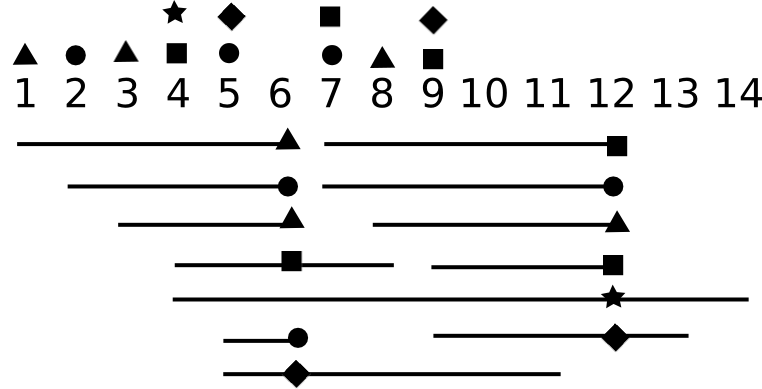
\includegraphics[width=.7\linewidth]{other/jrp}
\caption{Example of running algorithm. Here the delay cost is unit cost, $K = 5$, fix ordering cost: triangle 2, circle 2, rectangle 4, star 10, diamond 6}
\end{figure}

\begin{lemma}
For inactive demand $(i,t)$ such that $\alpha(i,t)$ is strictly smaller than $\beta(i,t)$, there is no order within $(\alpha(i,t), \beta(i,t)]$. \label{lem:overlap}
\end{lemma}
\begin{proof}
The only case when $\alpha(i,t) < \beta(i,t)$ happens is when $(i,t)$ is included in an augmented order. In that case, remember that we put order at the time of last order. Suppose there is order within $(\alpha(i,t), \beta(i,t)]$, it must be already there when the Event II happens because we only place totally new order at current time. This contradict our choice to augment order at latest order available.
\end{proof}

For the sake of notation, let's define $\hat s_i$ to be the time of last order including $i$.

\begin{lemma}
In Event I for tight set $(S,s)$, the tight time $s$ is strictly larger than $\hat s_i$ for any $i\in S$. In Event II for $(i,s)$, $s$ is strictly larger than $\hat s_i$. \label{lem:larger}
\end{lemma}
\begin{proof}
In Event I, $s > \hat s$ so $s > \hat s_i$ trivially. In Event II, there is at least one active demand $(i,t)$ of type $i$ contributing. This implies $s \ge t$, we also know that since $(i,t)$ is active $t > \hat s_i$ because otherwise it's already served and must be inactive. Thus, $s > \hat s_i$.
\end{proof}

\begin{lemma}
For inactive demand $(i,t)$, it can be charged in the future only if $\alpha(i,t) = \hat s_i$. \label{lem:charge}
\end{lemma}
\begin{proof}
Suppose $(i,t)$ is served by order earlier than $\hat s_i$. Suppose in the future we place some order for tight set $(S,s)$. If item $i$ is involved, then because there is at least one active contributing demand of type $i$, we know $s > \hat s_i$. While for $(i,t)$, by Lemma \ref{lem:overlap}, there is no order within $(\alpha(i,t), \beta(i,t)]$, it must be that $\hat s_i > \beta(i,t)$ which implies $(i,t)$ cannot contributes to $(S,s)$.
\end{proof}

\begin{lemma}
Our charging scheme charged enough to pay for order cost.
\end{lemma}
\begin{proof}
For each contributing order $(i,t)$, we charged $Y(i,t,\alpha(i,t),\beta(i,t))$ for order cost but we actually need to charge$Y(i,t,s,\beta(i,t))$. So we just need to prove $\alpha(i,t) \le s$. For active order, since $\alpha(i,t) = t$, it's trivial. For inactive order, by Lemma \ref{lem:larger}, we know $s > \hat s_i \ge \alpha(i,t)$.
\end{proof}

Now we can prove our main theorem

\begin{theorem}
There exists a primal dual 2-approximation algorithm without pruning stage for Joint Replenishment Problem.
\end{theorem}
\begin{proof}
We prove this by showing an invariant of the algorithm. We want to show that at any time, all $y(i,t,s)$ such that $s < \hat s_i$ is charged at most twice and all $y(i,t,s)$ such that $s \ge \hat s_i$ is charged at most once.

The base case is trivial since we have no order at that time. Now suppose that the claim is true just before we place a new or augment order. We just need to prove claim is true for any demand involved after we place the order.

If we are placing a new order, then we charged any active contributing demand $(i,t)$ twice its total dual, but since after we place the order, we will update $\hat s = \hat s_i = \tau$, the claim is true for $(i,t)$. For inactive contributing demand $(i,t)$, by Lem \ref{lem:charge} we know that, $\alpha(i,t) = \hat s_i$. We're going to charge it  $Y(i,t,\alpha(i,t),\beta(i,t))$ then update $\hat s_i = \hat s$, which is strictly larger than $\beta(i,t)$ because it's Event I. By induction assumption, we know the claim is true for $(i,t)$.

If we are placing a augment order, for active demand $(i,t)$, we charge every $y(i,t,s)$ such that $s < \hat s$ twice and every $y(i,t,s)$ such that $s > \hat s$ once, which will satisfy our claim. For inactive demand $(i,t)$, we will charge it $Y(i,t,\alpha(i,t),\beta(i,t))$. By assumption, this part is only charged once before. Then we will update $\hat s_i = \hat s$, which is strictly larger than $\beta(i,t)$ by Lem \ref{lem:overlap}.
\end{proof}


\section{Submodular Joint Replenishment Problem}
%%%%%%%%%%%%%%%%%%%%%%%%%%%%%%%%%%%%%%%%%%%%%%%%%%
\subsection{Problem statement}
Submodular Joint Replenishment Problem is a inventory problem. We have a shop, which holds inventory for a number of items. There are deterministic demands we need to satisfy for discrete time $1,2,\ldots, T$, where $T$ the time horizon. There are $n$ items and we index them by $\{1,2,\ldots, n\}$. In order to satisfy these demand, we can put orders at some time and they can be used to satisfy demand of later time. If we use a order at time $s$ to satisfy demand at a later time $t$ for item $i$, the holding cost we incurred is $H^i_{st}$. To model the order cost, we use a submodular ordering cost function $f(U)$. If we put a order at $s$ consisting a subset of items $U \subseteq [n]$, then we incur order cost $f(U)$.

There are some assumptions we need for this problem. The holding cost $H^i_{st}$ is defined for $s = 1,2,\ldots, t$ and non-increasing for $s$. Also the order cost $f(U)$ is a monotone submodular function, and we assume $f(\emptyset) = 0$.

%%%%%%%%%%%%%%%%%%%%%%%%%%%%%%%%%%%%%%%%%%%%%%%%%%
\subsection{Linear Programming Relaxation}
The linear programming relaxation of this problem is the following,

\begin{align*}
\min		\quad 	& \sum f(U) y^U_s + \sum H^i_{st}x^i_{st} \\
\text{s.t.}	\quad	& \sum_s x^i_{st} = 1 \\
				& x^i_{st} \le \sum_{U \ni i} y^U_s \\
				& x^i_{st} \ge 0
\end{align*}

Here $x^i_{st}$ is the variable indicating whether we use a order at time $s$ to satisfy order $(i,t)$. We use $y^U_s$ to denote whether we put a order consisting of items $U$ at time $s$.

%%%%%%%%%%%%%%%%%%%%%%%%%%%%%%%%%%%%%%%%%%%%%%%%%%
\subsection{LP based approximation algorithm}
In this section, we describe how we can use the optimal LP solution to simply the problem. First of all, this LP is of exponential number of variables, but we can use ellipsoid method to solve the dual by using submodular function minimization for separation.

Suppose we solve the LP and obtain optimal fractional solution $\bar y^U_s, \bar x^i_{st}$. Let's first look at some structure of optimal fractional solution. Let $\bar z^i_s = \sum_{i \ni U} \bar y^U_s$ and we can think about this as the fractional service we provided for item $i$ at time $s$.

\begin{lem}
Fix some time $s$ and then order all items such that $\bar z^1_s \ge \bar z^2_s \ge \cdots \ge \bar z^n_s$. Denote $U_i = \{1,2,\ldots, i\}$, then

\begin{enumerate}
\item $\bar y^{U_i}_s = \bar z^{i+1}_s - \bar z^i_s$ for $i=1,2,\ldots, n$ and $\bar y^U_s = 0$ for all other $U$.
\item $\bar z^i_s = \max_t \bar x^i_{st}$
\end{enumerate}
\end{lem}

The proof of this lemma is by the greedy algorithm for polymatroid optimization and by fixing $\bar y^U_s$ or $\bar x^i_{st}$ and looking at the other one.

Now let's focus on some item $i$. Let's spread out $\bar z^i_s$, and thus $\bar y^U_s$, over time $[s, s+1]$ uniformly. Then we partition the the time $[1, T+1]$ into disjoint intervals $(a_j, b_j]$ such that each interval (possibly except the last one) has mass $0.5$. For item $i$, denote the set of interval $I_i$.

Now, with the set of intervals $I_i$ for $i \in [n]$, we can construct a restricted instance of submodular JRP-D. We have all these intervals over time $[1, T+1]$ to stab and at any time if we put a order of subset $U$, it will stab all the intervals for items in $U$. Here we relax the requirement to put order at discrete time and we can put orders at any time (but it turns out to be that it only makes sense to put order at some interval's right endpoint).

\begin{lem}
With a feasible solution of the JRP-D instance, we can construct a feasible solution to our original JRP instance with ordering cost no more than the cost of JRP-D and holding cost less than LP-OPT.
\end{lem}
\begin{proof}
For a order at time $s$ for subset $U$, we round it to be at time $\lfloor s \rfloor$. Then every demand $(i,t)$ must be satisfied by some order in its active interval $[s_1, t]$, where $s_1$ is the earliest time such that $\bar x^i_{st} > 0$.
\end{proof}

Let the set of right endpoints of any interval in any $I_i$ be $P$ and we number them as $1,2,\ldots, T$. Since it's only sensible to put a order at some time in $P$, we can convert all the interval into the form of $(a, b]$ where $a,b \in P$.

\begin{lem}
We can convert the fractional solution $\bar y, \bar z$ of JRP to a fractional solution $\hat y, \hat z$ to JRP-D by aggregate all mass of $\bar y, \bar z$ between $(s, s+1]$ to time $s+1$. Then $2\hat y, 2\hat z$ will be a feasible solution to JRP-D. This implies that LP-OPT' is at most twice LP-OPT.
\end{lem}

This implies if we can devise a $\alpha$-approximation algorithm for JRP-D, then we can obtain $2\alpha+1$-approximation algorithm for JRP.

%%%%%%%%%%%%%%%%%%%%%%%%%%%%%%%%%%%%%%%%%%%%%%%%%%
\subsection{$\log n$-approximation algorithm for JRP-D}
The restricted JRP-D problem we want to solve can be explicitly stated. We have $n$ items and each corresponds to a partition of time horizon $(1,T]$ into disjoint intervals of form $(a,b]$ where $a,b$ are both integers. We can put orders at integer times to stab these intervals. To put a order with the ability to stab the intervals of set of items $U$, we need to pay $f(U)$ cost. We are interested in finding the least costly way to stab all intervals.

We can view this problem as a SET COVER problem by interpreting all intervals as elements to be covered. We index all set by the time of the order $s$ and the subset of items included $U$. The set $(s, U)$ will include all intervals which include $s$ and corresponds to items $U$. Note that at any time $s$, there are exactly $n$ intervals and each corresponds to one item.

We can apply the greedy algorithm on this problem and guarantee would be $\log n$ because any set contains at most $n$ elements. The ability to perform such greedy algorithm depends on our ability to solve
\[	\min_{U \subseteq A} f(U)/|U|	\]
where $A$ is the set of active (uncovered) intervals at some time $s$. This can be solved by the push-relabel submodular function minimization algorithm as a parametric SFM with discrete Newton method. We enumerate $s$ to find the most economic choice and pick that set.
\section{Simple rounding algorithm for soft-capacity multiple items lot-sizing
problem with constant opening cost}

\subsection{Problem statement}

Here we are considering multiple-items lot-sizing problem with
soft capacity. The assumption we are making here is that
the ordering cost is the same across time periods.

More specifically, we have time horizon $T$ and each time period
$s$ is associated with a capacity $C_s$. There are $N$ different
items and item $i$ has demand $d_{it}$ at time period $t$. If we
use order at time $s$ to satisfy demand at $t$ for item $i$,
per unit holding cost is $h_{st}^i$. For each time period $s$,
if we open it, the opening cost is $K$ and we can at most satisfy
$C_s$ units of demand from it. However, in the soft capacity
variant, we can open a time period multiple times.


\subsection{Linear Programming forumulation}

We use decision variables $y_s$ to denote how many copies do we
open order at time period $s$ and $x_{st}^i$ to denote the fraction of
demands $d_{it}$ served by orders at $s$. Then the following is
a natural linear programming

\begin{align*}
\min \quad    & K\sum_s y_s + \sum_{i,t}\sum_{s\le t}
                d_{it}h_{st}^i x_{st}^i   \\
\text{s.t.} \quad  & x_{st}^i \le y_s          \\
              & \sum_s x_{st}^i = 1       \\
              & \sum_{i,t} d_{it}x_{st}^i \le C_s y_s \\
              & x \ge 0, y \ge 0
\end{align*}


\subsection{Rounding algorithm}

We know that if opening cost is allowed to vary according
to time period. Then the natural LP has unbounded integrality
gap. Here we provide a rounding algorithm for the case
with fixed ordering cost, which also proves the integrality
gap of LP is constant.

First, we solve the linear programming and get optimal
fractional solution $x^*, y^*$. Then we modify $x^*$
to flow-requirement $z$ in following way:
for a fixed demand $(i,t)$, we look at its fractional
assignment, we remove the last $.75$ of it and quadruple
the first $.25$ of it. Now for each requirement $z_{st}^i$,
if we can satisfy it within orders between $s$ and $t$
inclusively, then the holding cost is at most $4$ times
of the fractional holding cost.

Now we describe how to round $y$. We put all $y^*$ on the number
axis, then moving from left to right, for every interval of
length $.25$, we open the one with largest capacity. In the end,
is there is any remaining, we just discard it. Clearly,
the total opening cost is at most $4$ times of the fractional
opening cost.

Now, we just need to prove there is a feasible assignment
that satisfies requirement $z$ and capacity constraints.

Here, we run the Median Assignment Algorithm in Lordi paper.
Again, we want to show the algorithm will success. Suppose
on the contrary, the algorithm fails with some requirement
$z^i_{\tau\bar t}$. Still let $\bar r$ be the earliest period that
still has free capacity and let $F = [\tau, \bar r)$. Let $A$
be all demands within $F$ such that it has positive flow-requirement
within $F$. By similar argument, we know that all capacity
in $F$ is used to satisfy $A$ and there isn't enough. We
want to prove the opposite, that we do have enough capacity.

\begin{claim}
There is enough capacity in $F$ to satisfy requirement in $A$.
\end{claim}

\begin{proof}
First, we look at $F$, and we claim that it opened capacity
at least four times the fractional capacity within $[\tau+.25,\bar r-.25)$.
By construction of the algorithm, it at most assigns the first .25 and the
last .25 to some order outside $F$. For everything else, it opens
at least four times.

Now, take any demand $(i,t)$, because it has positive
flow-requirement within $F$, it must has at least .75 fractional
assignment within $F$. Thus, the intersection of its fractional
assignment and $[\tau+.25,\bar r-.25)$ is at least .25. This
is true for any demand $(i,t) \in A$. So take all of them aggregately,
we know they all have at least .25 fractional assignment in $[\tau+.25,\bar r-.25)$.
So the total fractional capacity in $[\tau+.25,\bar r-.25)$ is at least a quarter
of the demands in $A$. But since we opened four times the fractional capacity
in $[\tau+.25,\bar r-.25)$, we know we have enough capacity.
\end{proof}

This leads to the main result

\begin{thm}
There is a 4-approximation to the soft-capacity version of multiple items lot-sizing
problem with constant opening cost. Moreover, the natural LP has integrality gap
at most 4.
\end{thm}
\paragraph{Problem}
We consider the scheduling problem $1 | r_j | \max W_j$.
In this problem, we have $n$ jobs and job $j$ has process time $p_j$ and release date $r_j$.
Without lose of generality, we can assume $r_1 \le r_2 \le \ldots \le r_n$.
We want to schedule these jobs on one machine.
Job $j$ cannot be started until its release date $r_j$, and it takes $p_j$ for the machine to process it.
We cannot preempt, i.e. once we start a job, we cannot stop it until it finish.

For each job $j$, let $C_j$ be its completion time,
then the waiting time $W_j = C_j - r_j - p_j$ is the duration it waits from release until get started.
We want to find a schedule that minimize the maximum waiting time experienced by any job.

\begin{thm}
There is a polynomial algorithm to solve $1 | r_j | \max W_j$
\end{thm}

\paragraph{Structural property}
First, let's consider the structure of optimal solution.
Let $S^*$ be the optimal scheduling and let $j$ be the last job in $S^*$.

\begin{lem}
If $i, k$ are two consecutive jobs in $S^*$ other than $j$ and $i > j, i > k$.
Then we can swap order of $i,k$ and reach a schedule with no worse objective.
\end{lem}
\begin{proof}
Suppose $i$ is started at time $t$ before swapping, then $t \ge r_i$.
Since $k$ is released before $i$, so $r_k \le r_i \le t$.
Let's do the swap and start $k$ exactly at time $t$ and then start $i$ at time $t + p_k$.
Before or after swap, both jobs will be completed by $t + p_i + p_k$.
Thus, it won't affect any job after them. Also, we don't need to change anything about jobs before them.

Thus, we only need to analyze what happens to the waiting time of $i,k$.
Since $k$ is moved forward, it's waiting time decrease. So it won't cause any problem.
For $i$, its waiting time increase, but let's compare it to that of $j$.
$i$ is released later than $j$ but is completed before $j$, thus, its waiting time is at most that of $j$.
Since $j$'s waiting time doesn't change, $i$'s new waiting time is bounded by $W_{max}$ of original schedule.
In other words, we can do the swap and the schedule won't be worse.
Of course, if there is any leeway and we can start $k$ earlier than $k$ before $t$,
then there is no point of not doing it. This may lead to a better overall schedule.
\end{proof}

By this lemma, what we can do is to repeatedly swap job $n$ backward until it's just before $j$.
Then we move $n-1$ backward until it's just before $n$.
In the end, we will be able to reach a ordering of $i_1, \ldots, i_{j-1}, j+1, \ldots, n, j$.
Here $i_1, \ldots, i_{j-1}$ is a permutation of jobs $1, \ldots, j-1$.
\section{Single machine scheduling to minimize maximum waiting time}
Let's call the tail $j+1, \ldots, n, j$ of this schedule a block. We can further invoke the lemma,
to decompose $i_1, \ldots, i_{j-1}$ into blocks.

\begin{cor}
The optimal schedule is of structure $S^* = B_1 \cdots B_k$, where each block consists of
some consecutive jobs in $1, \ldots, n$. In additional, each block will put the smallest
job in that block at the end and all other jobs in that block before that in natural order.

For example, if $S^* = 12453687$, then $B_1 = 1, B_2 = 2, B_3=453, B_4=6, B_5=87$. 
\end{cor}

\paragraph{Algorithm}
We will devise a procedure that, given a target maximum waiting time $W_{max}$, decide whether
there is a schedule achieve this target. With this, we can use binary search to find
the optimal $W_{max}$.

The procedure will be based on dynamic programming. Let $f(j)$ be the minimum makespan of
any schedule of jobs $1, \ldots, j$ such that each job wait at most $W_{max}$.
Let $f(0) = 0$.

For $j = 1,\ldots, n$, we can compute $f(j)$ as follows. Because we know the optimal schedule
of $1, \ldots, j$ consists of blocks, we can try to decide the last blocks.
We can try $i = 1, \ldots, j$ that the last block is $i+1, \ldots, j, i$. After deciding
the last block, how should we schedule jobs before that? As long as those jobs satisfy the
waiting time requirement, we just want to minimize their makespan so it's easier to
schedule the last block. As a result, we can
schedule jobs $1, \ldots, i-1$ with makespan $f(i-1)$ and then schedule jobs $i+1, \ldots, j, i$
in that ordering. Then, we examine whether job $i+1, \ldots, j, i$ satisfy the waiting time
requirement. Among all choice of last block satisfying waiting time requirement, we
pick the one with minimum makespan and that would be $f(j)$.

By definition, if there is any schedule of all jobs satisfying the waiting time requirement,
our DP algorithm will be able to find it. This completed our algorithm.

For our binary search, we need a upper bound of $W_{max}$ to begin with.
If we schedule jobs in order $1,\ldots, n$, it's easy to prove that any job waits
at most $P = \sum_{j=1}^n p_j$.
The overall running time is $O(n^3\log P)$.


\bibliography{chap1/ref,chap2/myrefs,chap3/ref}

\end{document}
